\documentclass[10pt]{article}
\usepackage[utf8]{inputenc}
\usepackage[T1]{fontenc}
\usepackage{graphicx}
\usepackage[export]{adjustbox}
\graphicspath{ {./images/} }
\usepackage{hyperref}
\hypersetup{colorlinks=true, linkcolor=blue, filecolor=magenta, urlcolor=cyan,}
\urlstyle{same}
\usepackage{amsmath}
\usepackage{amsfonts}
\usepackage{amssymb}
\usepackage{mhchem}
\usepackage{stmaryrd}

\title{Introduction to Operations Research and Mathematical Modeling }


\author{A Case Study Approach}
\date{}


\begin{document}
\maketitle

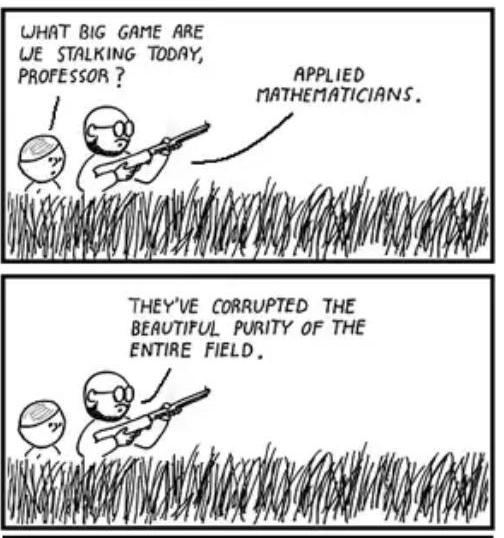
\includegraphics[max width=\textwidth]{2022_07_05_5945264bba2a5f6ba667g-01}

THOSE LRETCHED CREATURES HAVE INVADED EVERY BRANCH OF PURE MATH AND TURNED THEM INTO BRANCH OF PURE MATH AND TURNED\\
USEFUL REAL WORLD APPLICATIONS.


\includegraphics[max width=\textwidth]{2022_07_05_5945264bba2a5f6ba667g-01(1)}

(\href{http://tagg.org}{tagg.org}, n.d.)

Karin Vorwerk, Ph.D., Department of Mathematics, Westfield State University $\mathrm{~ A B O U T ~ T H I S ~ C L A S S ~ . . . . . . . . . . . . . . . . . . . . . . .}$

$\mathrm{~ W h a t ~ i s ~ O p e r a t i o n s ~ R e s e a r c h ~ . . . . . . . . . . . . . . . . .}$

$\mathrm{~ W h a t ~ i s ~ M a t h e m a t i c a l ~ M o d e l i n g ~ . . . . . . . . . . . . . . . . . . . . . . . . . . . . . . . . . . . . . . . . . . . . . . . . . . . . . . . . . . . . . . . . .}$

$\mathrm{~ T h e ~ C a s e ~ S t u d y ~ A p p r o a c h . . . . . . . . . . . . . . . . . . . . . . . . . . . . . .}$

$\mathrm{~ T o p i c s ~ C o v e r e d ~ . . . . . . . . . . . . . . . . . . . . . . . . . . . . . . . . . . . . . . . . . . . . . . . . . . . . . . . . . . . . . . . . . . . . .}$

$\mathrm{~ C l a s s ~ S c h e d u l e ~ . . . . . . . . . . . . . . . . . . . . . . . . . . . . . . . . . . . . . . . . . . . . . . . . . . . . . . .}$

$\mathrm{~ G r a d i n g ~ . . . . . . . . . . . . . . . . . . . . . . . . . . . . . . . . . . . . . . . . . . . . . . . . . . . . . . . . . . . . . . .}$

Resources $\ldots \ldots \ldots \ldots \ldots \ldots \ldots \ldots \ldots \ldots \ldots \ldots \ldots \ldots \ldots \ldots \ldots \ldots \ldots \ldots \ldots \ldots \ldots \ldots \ldots \ldots \ldots \ldots \ldots \ldots \ldots \ldots \ldots \ldots \ldots \ldots \ldots \ldots \ldots \ldots \ldots \ldots \ldots \ldots \ldots \ldots . \ldots$

$\mathrm{~ D E E R ~ P O P U L A T I O N S ~ - ~ P O P U L A T I O N ~ M O D E L S ~ . . . . . . . . . .}$

$\mathrm{~ L e a r n i n g ~ G o a l s ~ . . . . . . . . . . . . . . . . . . . . . . . . . . . . . . . . . . . . . . . . . .}$

$\mathrm{~ C a s e ~ S t u d y ~ D e s c r i p t i o n ~ - ~ D e e r ~ P o p u l a t i o n . . . . . . . . . . . . . . . . . . . . . . . . . . . . . . . . . . . . .}$

$\mathrm{~ R e f e r e n c e s . . . . . . . . . . . . . . . . . . . . . . . . . . . . . . . . . . . . . . . . . . . . . . .}$

$\mathrm{~ A ~ F i r s t ~ M o d e l ~ . . . . . . . . . . . . . . . . . . . . . . .}$

$\mathrm{~ I n t r o d u c i n g ~ C a r r y i n g ~ C a p a c i t y ~ . . . . . . . . . . . . . . . . . . . . . . . . . . . . . . . . . . . . . . . . . . . . . . . . . . . . . . . . . . . . . . . . . . . . . . . . . . . . .}$

$\mathrm{~ I n t r o d u c i n g ~ H u n t i n g ~ . . . . . . . . . . . . . . . . . . . . . . . . . . . . . . . . . . . . . .}$

$\mathrm{~ I n t r o d u c i n g ~ P r e d a t o r s ~ . . . . . . . . . . . . . . . . . . . . . . . . . . . . . . . . . . . . . . . . . . . . . . . . . . . . . . . . . . . . . . . . . . . . . . . . . . . . . . . . . . . . . .}$

Diagrams and Recursive Sequences - Multiple Populations........................................................ 16

COMPUTATING AREAS - SIMULATION $1 \ldots \ldots \ldots \ldots \ldots \ldots \ldots \ldots \ldots \ldots \ldots \ldots \ldots \ldots \ldots \ldots \ldots \ldots \ldots \ldots \ldots \ldots \ldots \ldots \ldots \ldots \ldots . \ldots \ldots \ldots \ldots \ldots \ldots \ldots \ldots \ldots \ldots \ldots \ldots \ldots \ldots \ldots \ldots \ldots \ldots$

Learning Goals ........................................................................................................ 18

$\mathrm{~ C a s e ~ S t u d y ~ D e s c r i p t i o n ~ - ~ C o m p u t i n g ~ A r e a s ~ . . . . . . . . . . . . . . . . . . . . . . . . . . . . . . . . . . . . . . . . . . . . . . . . . . . .}$

$\mathrm{~ S o l u t i o n ~ A p p r o a c h ~ . . . . . . . . . . . . . . . . . . . . . . . . .}$

MODELING THE SPREAD OF DISEASES - SIMULATION $2 \ldots \ldots \ldots \ldots \ldots \ldots \ldots \ldots \ldots \ldots \ldots \ldots \ldots \ldots \ldots \ldots \ldots \ldots \ldots \ldots \ldots \ldots \ldots \ldots \ldots \ldots \ldots \ldots . . \ldots \ldots$

$\mathrm{~ L e a r n i n g ~ G o a l s . . . . . . . . . . . . . . . . . . . . . . . . . . . . . . . . . . . . . . . . . . . . . . . . . . . . . . . . . . . . . . . . .}$

$\mathrm{~ C a s e ~ S t u d y ~ D e s c r i p t i o n ~ - ~ D i s e a s e s ~ . . . . . . . . . . . . . . . . . . .}$

$\mathrm{~ S o l u t i o n ~ A p p r o a c h . . . . . . . . . . . . . . . . . . . . . . . . . . . . . . . . . . . . . . . . . . . . . . . . . . . . . . . . . . . . . . . . . . . . . . . . .}$

$\mathrm{~ D E S I G N I N G ~ A ~ C A M P G R O U N D ~ - ~ S I M P L E X ~ M E T H O D ~ . . . . . . . . . . . .}$

$\mathrm{~ L e a r n i n g ~ G o a l s . . . . . . . . . . . . . . . . . . . . . . . . . . . . . . . . . . . . . . . . . . . . . . . . . . . . . . . . . .}$

Case Study Description - Campground ......................................................................... 26

$\mathrm{~ R e f e r e n c e s . . . . . . . . . . . . . . . . . . . . . . . . . . . . . . . . . . . . . .}$

$\mathrm{~ S o l u t i o n ~ A p p r o a c h ~ - ~ T w o ~ V a r i a b l e s ~ . . . . . . . . . . . . . . . . . . . . . . . . . . . . . . . . . .}$

Assumptions made about linear programming problem $\ldots \ldots \ldots \ldots \ldots \ldots \ldots \ldots \ldots \ldots \ldots \ldots \ldots \ldots \ldots \ldots \ldots \ldots \ldots \ldots \ldots \cdots \ldots \ldots \cdots \cdots \ldots \ldots \ldots \ldots \ldots \ldots \ldots \ldots \ldots \ldots \ldots \ldots \ldots \ldots \ldots \ldots \ldots \ldots \ldots$

$\mathrm{~ A s s u m p t i o n s ~ m a d e ~ a b o u t ~ l i n e a r ~ p r o g r a m m i n g ~ p r o b l e m ~ . . . . . . . . . . . . . . .}$

$\mathrm{~ G r a p h i c a l ~ S i m p l e x ~ s o l u t i o n ~ p r o c e d u r e ~ . . . w . w . w . w . w . w . w}$

$\mathrm{~ S t a t i n g ~ t h e ~ S o l u t i o n ~ . . . w . w . w . w . w . w . w}$

$\mathrm{~ R e f i n e m e n t s ~ t o ~ t h e ~ g r a p h i c a l ~ s o l u t i o n ~ . . . w . w . w . w . w . w .}$

$\mathrm{~ S o l u t i o n ~ A p p r o a c h ~ - ~ A l g e b r a i c ~ S i m p l e x ~ M e t h o d ~ . . . . . . w}$

$\mathrm{~ C o r n e r ~ p o i n t s , ~ i n t e r i o r ~ c o r n e r ~ p o i n t s , ~ s l a c k ~ v a r i a b l e s ~ . . . . . . . . . . . . . . . . . . . . . . . . .}$

$\mathrm{~ S o l v i n g ~ t h e ~ f u l l ~ p r o b l e m ~ . . . . . . . . . . . . . . . . . . . . . . . . . . . . . .}$

$\mathrm{~ S t a t i n g ~ t h e ~ s o l u t i o n ~ . . . . . . . . . . . . . . . . . . . . . . . . . . . . . . . . . . . . . .}$ $\mathrm{~ A ~ R e m a r k ~ o n ~ B I P ~ a n d ~ I n t e g e r ~ P r o g r a m m i n g . . . . . . . . . .}$

$\mathrm{~ A ~ F i n a l ~ C o m m e n t ~ . . . . . . . . . . . . . . . . . . . . . . . . . . . . . . . . . . . . . . . . . . . . . . . . . . . .}$

$\mathrm{~ N A T I O N A L ~ P A R K ~ - ~ N E T W O R K S ~ A N D ~ A S S I G N M E N T ~ . . . . . . . . . . . . . . . . . . . . .}$

$\mathrm{~ L e a r n i n g ~ G o a l s . . . . . . . . . . . . . . . . . . . . . . . . . . . . . . . . . .}$

$\mathrm{~ C a s e ~ S t u d y ~ D e s c r i p t i o n ~ - ~ N a t i o n a l ~ P a r k ~ . . . . . . . . . . . . . . . . . . . . . . . . . . . . . . . . . . . . . . . . . . . . . . .}$

$\mathrm{~ R e f e r e n c e s . . . . . . . . . . . . . . . . . . . . .}$

$\mathrm{~ P a r t ~ 1 : ~ W o r k ~ F o r c e ~ - ~ R e s o u r c e ~ A l l o c a t i o n . . . . . . . . . . . . . . . . . . . . . . . . . . . . . . . . . . . . . . . . . . . . . . . . . . . .}$

$\mathrm{~ R e f i n e m e n t s ~ . . . . . . . . . . . . . . . . . . . . . . . . . . . . . . . . . . . . . . . . . . . . . . . . . . . .}$

$\mathrm{~ S t a t i n g ~ t h e ~ s o l u t i o n ~ . . . . . . . . . . . . . . . . . . . . . . . . . . . . . . . . . . . . . . . . . . . . . . . . .}$

Part 2: Shuttle service - Shortest Path and Maximum Flow ...................................................46

$\mathrm{~ S h o r t e s t ~ P a t h ~ . . . . . . . . . . . . . . . . . . . . . . . . . . . . . . . . . . . . . . . . . . . . . . . . . . . .}$

$\mathrm{~ S t a t i n g ~ t h e ~ s o l u t i o n ~ . . . . . . . . . . . .}$

$\mathrm{~ M a x i m u m ~ F l o w . . . . . . . . . . . . . . . . . . . . . . . . . . . . . . . . .}$

$\mathrm{~ M a x i m u m ~ F l o w . . . . . . . . . . . . .}$

$\mathrm{~ M a x i m u m ~ F l o w ~ - ~ M i n i m u m ~ C o s t ~ . . . . . . . . . . . . . . . . . . . . . . . . . . . . . . . . . . .}$

$\mathrm{~ S t a t i n g ~ t h e ~ s o l u t i o n ~ . . . . . . . . . . . . . . . . . . . . . .}$

$\mathrm{~ S t a t i n g ~ t h e ~ s o l u t i o n ~ . . . . . . . . . . . . . . . . . . . . . . . . . . . . . . . . . . . . . . . . . . . . . . . . . . . . . . .}$

$\mathrm{~ P a r t ~ 4 : ~ D e l i v e r i e s ~ - ~ T r a v e l i n g ~ S a l e s m a n ~ P r o b l e m ~ . . . . . . . . . . . . . . . . . . . . .}$

$\mathrm{~ P a r t ~ 4 : ~ D e l i v e r i e s ~ - ~ T r a v e l i n g ~ S a l e s m a n ~ P r o b l e m ~ . . . . . . . . . . . . . . .}$

$\mathrm{~ N e a r e s t ~ N e i g h b o r ~ A p p r o a c h ~ . . . . . . . . . . . . . . . . . . . . . . . . . . . . . . . . . . . . . . . . . . . . . . . . . . . . . . . . .}$

$\mathrm{~ S u b - t o u r ~ R e v e r s a l ~ . . . w . w . w . w . w . w . w . w}$

$\mathrm{~ T S P ~ u s i n g ~ E x c e l ~ . . . . . . . . . . . . .}$

$\mathrm{~ S t a t i n g ~ t h e ~ S o l u t i o n ~ . . . . . . . . . . . . . . . . . .}$

Part 5: Road Patrols - Traversing $\ldots \ldots \ldots \ldots \ldots \ldots \ldots \ldots \ldots \ldots \ldots \ldots \ldots \ldots \ldots \ldots \ldots \ldots \ldots \ldots \ldots \ldots \ldots \ldots \ldots \ldots \ldots \ldots \ldots \ldots \ldots \ldots \ldots 59$

Stating the Solution $\ldots \ldots \ldots \ldots \ldots \ldots \ldots \ldots \ldots \ldots \ldots \ldots \ldots \ldots \ldots \ldots \ldots \ldots \ldots \ldots \ldots \ldots \ldots \ldots \ldots \ldots \ldots \ldots \ldots \ldots \ldots \ldots \ldots \ldots \ldots \ldots 60 . \ldots \ldots \ldots \ldots \ldots$

$\mathrm{~ G A S ~ E X P L O R A T I O N ~ - ~ D E C I S I O N ~ A N A L Y S I S ~ . . . . . . . . . . . . . . . . . . . . . . . . . . . . . . . . .}$

$\mathrm{~ L e a r n i n g ~ G o a l s . . . . . . . . . . . . . . . . . . . . . . . . . . . . . . . . . . . . . . . . . . . . . . . . . . . . . .}$

Case Study Description - Gas Exploration................................................................................ 61

$\mathrm{~ R e f e r e n c e s . . . . . . . . . . . . . . . . . . . . . . . . . . . . . . . . . .}$

$\mathrm{~ S o l u t i o n ~ A p p r o a c h . . . . . . . . . . . . . . . . . . . . . . . . . . . . . . . . . . . . . . . . . . . . . . . . . . . . . . . . . . . . . . . . . . . . .}$

$\mathrm{~ S t a t i n g ~ t h e ~ S o l u t i o n ~ . . . . . . . . . . . . . . . . . . . . . . . . . . . . . . . . . . . . . . . . . . . . . . . . . . . . . . . . . . . . . . . .}$

$\mathrm{~ R O C K ~ P A P E R ~ S C I S S O R S ~ - ~ G A M E ~ T H E O R Y ~ . . . . . . . . . . . . . . . . . . . . . . . . . . . .}$

$\mathrm{~ L e a r n i n g ~ G o a l s . . . . . . . . . . . . . . . . . . . . . . . . . . . . . . . . . . . . . . . . . . . . . . . . . . . . . . . . . . . . . . . . . . . . . . . . . . . . . . . .}$

$\mathrm{~ C a s e ~ S t u d y ~ D e s c r i p t i o n ~ - ~ R o c k ~ P a p e r ~ S c i s s o r s . . . . . . . . . . . . . . . . . . . . . . . . . . . . . . . . . . . . . . . . . . . . . . . . . . . . .}$

References $\ldots \ldots \ldots \ldots \ldots \ldots \ldots \ldots \ldots \ldots \ldots \ldots \ldots \ldots \ldots \ldots \ldots \ldots \ldots \ldots \ldots \ldots \ldots \ldots \ldots \ldots \ldots \ldots \ldots \ldots \ldots \ldots \ldots \ldots \ldots \ldots \ldots \ldots \ldots \ldots \ldots \ldots \ldots \ldots \ldots \ldots \ldots \ldots \ldots \ldots 66$

Solution Approach $\ldots \ldots \ldots \ldots$

$\mathrm{~ M a x i m i z i n g ~ e x p e c t e d ~ r e t u r n ~ . . . . . . . . . . . . . . . . . . . . . . . . . . . . . . . . . . . . . . . . . . . . . . . . . . . . . . . . . . . . . . . . . . . . . . . . . . . . . . . . . . . . . . . . . . . 6}$

Minimizing potential loss ......................................................................................68

$\mathrm{~ S a d d l e ~ p o i n t s ~ . . . . . . . . . . . . . . . . . . . . . . . . . . . . . . . . . . . . . . . . . . . . . . . . . .}$

$\mathrm{~ D o m i n a t e d ~ s t r a t e g i e s ~ . . . . . . . . . . . . . . . . . . . . . . . . . . . .}$

$\mathrm{~ D o m i n a t e d ~ s t r a t e g i e s ~ . . . . . . . . . . . .}$

Stating the Solution $\ldots \ldots \ldots \ldots \ldots \ldots \ldots \ldots \ldots \ldots \ldots \ldots \ldots \ldots \ldots \ldots \ldots \ldots \ldots \ldots \ldots \ldots \ldots \ldots \ldots \ldots \ldots \ldots \ldots \ldots \ldots \ldots \ldots \ldots \ldots \ldots \ldots \ldots \ldots \ldots \ldots \ldots \ldots \ldots$ $\mathrm{~ B R A N D ~ L O Y A L T Y ~ - ~ M A R K O V ~ C H A I N S ~ . . . . . . . . . . . . . . .}$

$\mathrm{~ L e a r n i n g ~ G o a l s . . . . . . . . . . . . . . . . . . . . . . . . . . . . . . . . . . . . . . . . . . .}$

$\mathrm{~ C a s e ~ S t u d y ~ D e s c r i p t i o n ~ - ~ B r a n d ~ L o y a l t y ~ . . . . . . . . . . . . . . . . . . . . . . . . . . . . . . . . . . . . . . . . . . . . . . . . . . . . . . . . . . . . . . . . . . . . . . . . . .}$

$\mathrm{~ R e f e r e n c e s . . . . . . . . . . . . . . . . . . . . . . . . .}$

$\mathrm{~ S o l u t i o n ~ A p p r o a c h ~ . . . . . . . . . . . . . . . . . . . . . . . . . . . . . . . . . . . . . . . . . . . . . . . . . . . . . . . . . . . . . . . . . . . . . .}$

$\mathrm{~ N o t a t i o n ~ . . . . . . . . . . . . . . . . . . . . . . . . . . . . . . . . . . . . . . . . . . . . . . . . . . . . . . . . .}$

$\mathrm{~ P a r t ~ 1 : ~ S t a t u s ~ Q u o ~ . . . . . . . . . . . . . . . . . . . . . . . . . . . . . . . . . . . . . . . . . . . . . . . . . . . . . . . . . . . . . . . . . . . . . . . . . . . . . . . . . . . . . . . . . .}$

$\mathrm{~ S t a t i n g ~ t h e ~ S o l u t i o n ~ . . . . . . . . . . . . . . . . . . . . . . . .}$

$\mathrm{~ P a r t ~ 2 : ~ I n c r e a s e ~ C u s t o m e r ~ L o y a l t y . . . w . w . w . w}$

$\mathrm{~ S t a t i n g ~ t h e ~ S o l u t i o n ~ . . . . . . . . . . . . . . . . . . . . .}$

$\mathrm{~ P a r t ~ 3 : ~ A t t r a c t i n g ~ N e w ~ C u s t o m e r s . . . . . . . . . . . . . . . . . . . . . . . . . . . . . . . . . . . . . . . . . . . . . . . . . . . . . . . . . . . . . . . . . . . . . . . . . . .}$

$\mathrm{~ S t a t i n g ~ t h e ~ S o l u t i o n ~ . . . . . . . . . . . . . . . . . . . . . . . . . . . . . . . . . . . . . . . . . . . . . . . . . . . . . . . . . . .}$

A Final Comment ......................................................................................................... 79

$\mathrm{~ A P P E N D I C E S ~ . . . . . . . . . . . . . . . . . . . . . . . . . . . . . . . . . . . . . . . . . . . . . . . . . . . . . . . . . .}$

A1: How to Write a Request for Proposals............................................................................ 80

$\mathrm{~ A 2 : ~ S e l e c t e d ~ T o p i c s ~ f o r ~ P r o p o s a l s ~ . . . . . . . . . . . . . . . . . . . . . . . . . . . . . . . . . . . . . . . . . . . . . . . . . . .}$

$\mathrm{~ A 3 : ~ R e f e r e n c e s ~ . . . . . . . . . . . . . . . . . . . . . . . . . . . . . . . . . . . . . . . . . . . . . . . . . . . . . . . . . . . . . . . . . . . . . . . . . . . . . . . . . . . . . . . . . . . . . . . . . .}$

$\mathrm{~ A 4 : ~ A c k n o w l e d g e m e n t s . . . . . . . . . . . . . . . . . . .}$

$\mathrm{~ A 5 : ~ I n d e x ~ . . . . . . . . . . . . . . . . . . .}$

\section{$\underline{\text { ABOUT THIS CLASS }}$}
This course is intended as a first introduction to Operations Research and Mathematical Modeling, and to give students an early exposure to Applied Mathematics. By the end of this course, students should have gained an understanding of the wide applicability and interdisciplinary nature of Operations Research and Mathematical Modeling. Students are invited to continue exploring through Independent Studies and/or research projects; see me if you are interested.

This course is designed for sophomores or higher, I assume students have completed Calculus 1 and 2 , Linear Algebra, and ideally a Statistics course. However, it should be possible for students to fill in any gaps they may have.

Much of OR and Mathematical Modeling involves the use of programming and computers. For the relatively problem we will study Excel is a powerful, readily available, and common tool. Excel skills learned in this class should be readily transferrable to other applications and future jobs. I do not expect any of you to have any Excel skills, you will learn what you need in class.

Operations research is frequently viewed as a discipline in itself, not just as a branch of mathematics. An introductory, one semester course in Operations Research and Mathematical Modeling can only give an overview. I have attempted to cover many of the central ideas, topics, and solution approaches, but had to omit others and some of the more technical details.

By necessity, I have simplified and streamlined much of the material. Vocabulary is kept simple. While it is important for me that you understand why procedures and algorithms work, we will stress the applied side of Mathematics and keep proofs to a minimum. I am happy to provide additional theoretical background to those students who are interested.

\section{What is Operations Research}
Operations Research can be defined as a he application of scientific and analytic methods to the management of organizations and businesses, providing a quantitative basis for problem-solving and making complex decisions.

Operations Research is yet another example of scientific progress being initiated by military applications and then adapted to civilian use. The beginnings of Operations Research are generally recognized as having initiated in England during WWII, when British scientists set out to make decisions regarding the best use and allocations of scarce resources to various military operations. After the war, their ideas were transferred to the civilian sector and further developed to increase efficiency and productivity. OR is concerned with the practical management of organizations. To be successful, you have to be able to clearly communicate your solution(s) to the decision makers in that organization.

A OR study of a problem may involve mathematics, statistics, probability theory, computer science, economics, psychology, maybe politics, and of course an understanding of the area the problem was derived from. Therefore, OR studies usually involve a team of individuals with a range of diverse backgrounds and skills.

A OR study of a problem may involve mathematics, statistics, probability theory, computer science, economics, psychology, maybe politics, and of course an understanding of the area the problem was derived from. Therefore, OR studies usually involve a team of individuals with a range of diverse backgrounds and skills.

\section{What is Mathematical Modeling}
By now it should be obvious that OR is concerned with solving real life problems using Mathematics. Thus, it is necessary to translate these problems into mathematical terms, the process we call mathematical modeling. The majority of applications will involve varying degrees of approximations and simplifications. Rather than considering all variables and influences, the modeler has to concentrate on the dominant variables that control the behavior of the real system.

There are three phases to mathematical modeling:

\begin{enumerate}
  \item Model construction
\end{enumerate}
This entails the translation of your real-world problem into mathematical terms. If you are lucky, then there exist standard models (for example for population growth).

\begin{enumerate}
  \setcounter{enumi}{2}
  \item Model solution
\end{enumerate}
This is usually the easy, or at least well-defined step. You will use mathematical methods you learn in class to solve your problem.

\begin{enumerate}
  \setcounter{enumi}{3}
  \item Model validation
\end{enumerate}
You have to check whether your model "makes sense", i.e. does the model adequately predict the behavior of the system under study. Are the results intuitively acceptable? A common method for checking the model is to compare model output to historical data, or, if no such data is available, to use simulation to validate the model output.

\section{The Case Study Approach}
In Applied Mathematics, usually the problem comes first, then potential solution approaches are explored. For this reason, we use a case study approach. Different, somewhat realistic scenarios are used to motivated different solution methods, rather than introducing a solution process first and then demonstrating it on a problem. In addition, students will work on their own case studies in groups. Each group will act as client for their own problem and as consultant for another group's problem. Instead of exams and a final, students will submit three intermediate reports, a final report, and give a final presentation.

In this class, we will define two groups:

\begin{enumerate}
  \item The clients pose the problem to be investigated and solved. The clients will write a request for proposals (see appendix) soliciting consultants to work for them. It is the clients' responsibility to provide all the constraints and a clear definition of the problem, to help the consultant understand the parameters and boundaries involved, and to ultimately judge the proposed solution and final product.

  \item The consultants will work on the actual problem and suggest a best solution (a characteristic of OR is that there may not be a perfect solution, but rather one or more solutions tied for best). While the consultant team must deal with all the technical (i.e. mathematical) aspects of the problem, the final report and proposed solution need to be phrased in terms appropriate to the original problem and understandable to lay people.

\end{enumerate}
\section{Topics Covered}
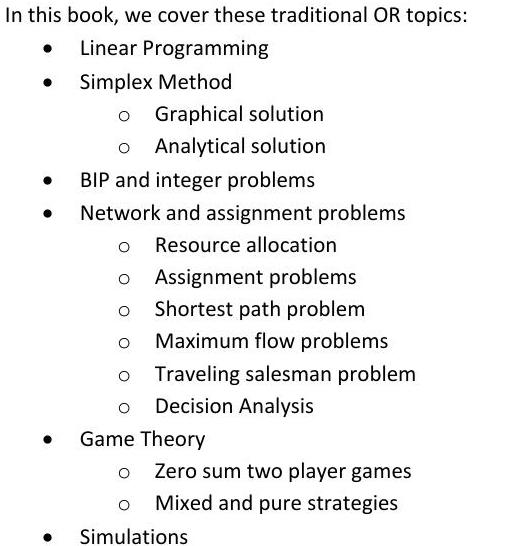
\includegraphics[max width=\textwidth]{2022_07_05_5945264bba2a5f6ba667g-07}

Mathematical Modeling topics:

\begin{itemize}
  \item Population models

  \item Exponential growth

  \item Logistic growth

\end{itemize}
o Predator-prey models

\begin{itemize}
  \item Spread of diseases

  \item Translating OR problems into mathematical form

\end{itemize}
Additional topics may be included as the class' interests dictate.

\section{Class Schedule}
The table below shows the due dates for the reports etc. Note that homework is not included in this list. It is your responsibility to know what was assigned and when. If you miss class, you need to either get the notes from a friend or come talk to me.

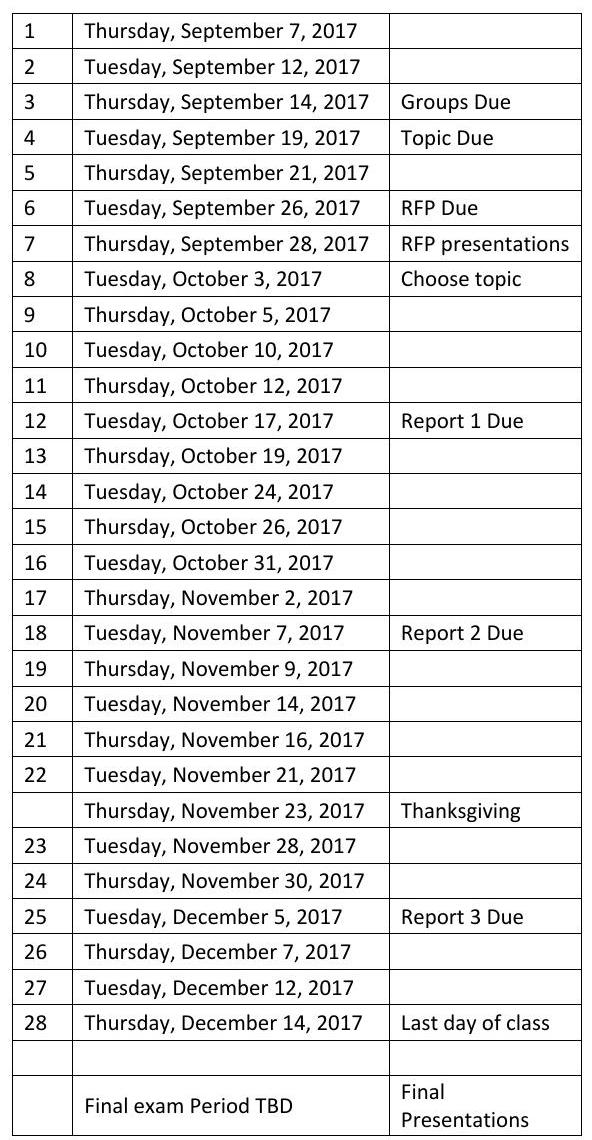
\includegraphics[max width=\textwidth]{2022_07_05_5945264bba2a5f6ba667g-08}

\section{Grading}
There are no exams in this class. Instead, you will be graded on weekly homework relating to the material covered in class a, your reports, your final presentation, and your final paper. Each group will rate the participation and contribution of its members and grade their clients work according to rubrics handed out in class.

Homework: $\quad 30$

RFP: $\quad 10$

Three reports 25

Final report 25

Final presentation 10

\section{Resources}
Appendix 3 contains a list of books you may find helpful, and are welcome to borrow for a few days (or get through the inter library loan system ILL). My favorite OR book is (Hillier \& Lieberman, 2005). This classic is also the most comprehensive and detailed text I know of. It covers every topic (except the first three chapters) in much detail and is an excellent reference. There is a wealth of actual case studies included.

If you are looking for a more technical reference, you should have a look at (Marlow, 2012). Originally copyrighted in 1978 , the updated 2012 version still retains that traditional math book feel. Another book I like to refer to is (Taha, 2003).

We will be using Excel a lot, and you will (have to) become very familiar with it. Each chapter will introduce you to some of the techniques we will be using in this class. Make sure you are able to reproduce all the spreadsheets we create in class. When in doubt, ask. Because Excel changes/updates every few years, and most likely people will work with different versions of it, your spread sheets may look different from mine. You will need to attend class to learn this. An excellent, although somewhat dated resource is (Neuwirth \& Arganbright, 2004).

Finally, I am happy to make this book available to you as a PDF and share my Excel files with you.

\section{DEER POPULATIONS - POPULATION MODELS}
\section{Learning Goals}
In this chapter, we will first develop a simple population model and then refine it to include carrying capacity, harvest, and predation. In addition, you will learn how to use Excel. In Excel, you should be able to:

\begin{itemize}
  \item Enter and copy formulas

  \item hold a parameter fixed

  \item create and customize a scatter plot

  \item customize your ribbon

  \item manage add-ins

  \item Insert a scroll bar (form control)

  \item Use Goal Seek

\end{itemize}
\section{Case Description - Deer Population}
In the fictitious county of Taxfield a debate is going on about how best to manage the deer herd. Currently, the deer population stands at about 60 deer per square mile, as urban development has created the habitat deer thrive in and people also feed deer in the winter months. The natural (i.e. no feeding) density is 20 deer per square mile (dpsm), the desired density is around 15 deer per square mile. You are to develop a model for the deer population that allows to model the effects of various management options (hunting, introducing predators). Taxfield county has an area of 877 square miles.

\section{$\underline{\text { References }}$}
For further reading on deer and coyote/coywolf, see the following websites:

\href{http://www.georgiawildlife.com/DeerFacts}{http://www.georgiawildlife.com/DeerFacts}

\href{http://www.theridgefieldpress.com/44515/deer-count-shows-dense-population/}{http://www.theridgefieldpress.com/44515/deer-count-shows-dense-population/}

\href{http://www.easterncoyoteresearch.com/easterncoyotelifecycle/}{http://www.easterncoyoteresearch.com/easterncoyotelifecycle/} \href{http://www.petersenshunting.com/predators/are-coyotes-killing-your-deer/}{http://www.petersenshunting.com/predators/are-coyotes-killing-your-deer/}

\section{$\underline{\text { A First Model }}$}
We will first assume that our deer population has unlimited room and feed and is not affected by predators, hunting, cars, etc. In this case, the rate at which your herd grows is entirely dependent on how many deer you have.

We introduce the variables $\mathrm{t}$ : time

$D(t): \quad$ number of deer at time $t$

r: $\quad$ growth rate of deer (a combination of births and deaths)

h: time step Using notation from calculus, we get:
$$
\frac{\text { change in } D(t)}{\text { change in } t}=r \cdot D(t)
$$
You may know that the solution is $D(t)=D(0) \cdot e^{r t}$. But we are trying to model/solve this with Excel. This means that we need to take the continuous problem and translate it into a discrete formulation. Recall the difference quotient definition of the derivative:
$$
D^{\prime}(t)=\lim _{h \rightarrow 0} \frac{D(t+h)-D(t)}{h},
$$
which means that $D^{\prime}(t) \approx \frac{D(t+h)-D(t)}{h}=r \cdot D(t)$ if $h$ is very small
$$
\begin{aligned}
&D(t+h) \approx D(t)+h \cdot D^{\prime}(t) \\
&D(t+h) \approx D(t)+h \cdot r \cdot D(t)
\end{aligned}
$$
Solving for $D(t+h)$ gives

Note: You may recognize this as the equation of the tangent line, or the linear approximation of $D(t)$, or the first two terms of the Taylor series.

Another note: Not surprisingly, when replacing the derivative by its approximation, we introduce an error into our model. In addition, there may be rounding errors, cut-off errors, and others. The field of Numerical Analysis deals with quantifying and controlling these and other errors.

In this set-up, $D(0), h$, and $r$ are parameters that we would like to be able to change without having to change our formula. In class, we created a spreadsheet that allows us to do just that. As a reminder, here is a copy showing the formulas used. Note that the graph shows exponential growth as expected.

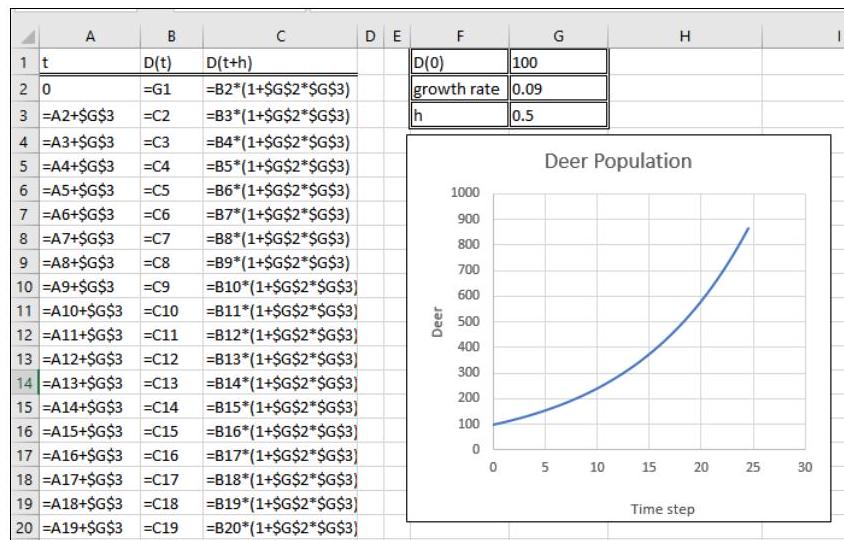
\includegraphics[max width=\textwidth]{2022_07_05_5945264bba2a5f6ba667g-11}

\section{Introducing Carrying Capacity}
If you think about it, the exponential growth model is not realistic. According to that model, the population would grow faster and faster without bound. In reality, you will run out of space, food, and patience long before then. The maximum sustainable number of deer, given the natural environment, is called the carrying capacity C. We need to change our basic model to reflect that

\begin{itemize}
  \item The population will grow if you have less deer than the carrying capacity, i.e. $\mathrm{D}^{\prime}(\mathrm{t})>0$ if $D(t)<C$

  \item The population will shrink if you have more deer than the carrying capacity, i.e. D'(t) $<0$ if $D(t)<C$

  \item The population will be stable if you either have no deer (duh) or exactly the right number $-$ carrying capacity, i.e. $D^{\prime}(t)=0$ if $D(t)=0$ or $D(t)=C$.

\end{itemize}
We will do so by adjusting our original equation by a factor of $C-D(t)$ :
$$
D^{\prime}(t)=r \cdot D(t) \cdot(C-D(t))
$$
We again replace $D^{\prime}(t)$ with the approximation $\frac{D(t+h)-D(t)}{h}$ and solve for $D(t+h)$.
$$
\begin{aligned}
& \frac{D(t+h)-D(t)}{h}=r \cdot D(t) \cdot(C-D(t)) \\
\leftrightarrow \quad D(t+h)=D(t)+h \cdot r \cdot D(t) \cdot(C-D(t))
\end{aligned}
$$
$$
\begin{aligned}
& \leftrightarrow \quad D(t+h)=D(t)+h \cdot r \cdot D(t) \cdot(C-D(t))
\end{aligned}
$$
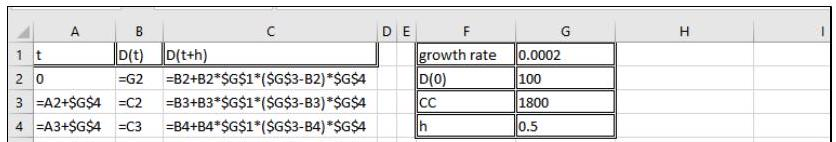
\includegraphics[max width=\textwidth]{2022_07_05_5945264bba2a5f6ba667g-12}

$5=A 4+\$ G \$ 4=C 4 \quad=B 5+B 5^{*} \$ G \$ 1^{*}(\$ G \$ 3-B 5)^{*} \$ G \$ 4$

$6=A 5+\$ G \$ 4=C 5 \quad=B 6+B 6^{*} \$ G \$ 1^{*}(\$ G \$ 3-B 6)^{*} \leqslant G \$ 4$

$7=A 6+\$ G \$ 4=C 6 \quad=B 7+B 7^{*} \$ G \$ 1^{*}(\$ G \$ 3-B 7)^{*} \$ G \$ 4$

$8=A 7+\$ G \$ 4=C 7 \quad=B 8+B 8^{*} \$ G \$ 1^{*}(\$ G \$ 3-B 8)^{*} \leqslant G \$ 4$

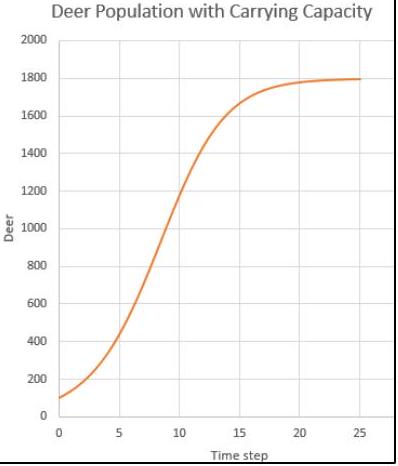
\includegraphics[max width=\textwidth]{2022_07_05_5945264bba2a5f6ba667g-12(1)}

$9=A 8+\$ G \$ 4=C 8 \quad=B 9+B 9^{*} \$ G 1^{*}(\$ G \$ 3-B 9)^{*} \$ G A$

$10=A 9+\$ G \$ 4=C 9 \quad=B 10+B 10^{*} \$ \$ \$ 1^{*}(\$ G \$ 3-B 10)^{*} \$ G \leqslant$

$11=A 10+\$ G \$ 4=C 10 \quad=B 11+B 11^{*} \$ G \$ 1^{*}(\$ G \$ 3-B 11)^{*} \$ G \leqslant$

$12 \mid=A 11+\$ G A=C 11=B 12+B 12^{*} \$ G \$ 1^{*}(\$ G \$ 3-B 12)^{*} \$ G G$

$13=A 12+\$ G \$ 4=C 12=B 13+B 13^{*} \$ G \$ 1^{*}(\$ G \$ 3-B 13)^{*} \$ G$ G

$14=A 13+\$ G \$ 4=C 13=B 14+B 14^{*} \$ G \$ 1^{*}(\$ G \$ 3-B 14)^{*} \$ G \leqslant$

$15=A 14+\$ G A 4=C 14=B 15+B 15^{*} \$ G \$ 1^{*}(\$ G \$ 3-B 15)^{*} \$ G$;

$16=A 15+\$ G \$ 4=C 15=B 16+B 16^{*} \$ G \$ 1^{*}(\$ G \$ 3-B 16)^{*} \$ G \leqslant$

$17=A 16+\$ G \$ 4=C 16=B 17+B 17^{*} \$ G \$ 1^{*}(\$ G \$ 3-B 17)^{*} \$ G$ G

$18=A 17+\$ G \$ 4=C 17=B 18+B 18^{*} \$ G \$ 1^{*}(\$ G \$ 3-B 18)^{*} \$ \$ G$

$19=A 18+\$ G \$ 4=C 18 \quad=B 19+B 19^{*} \$ G \$ 1^{*}(\$ G \$ 3-B 19)^{*} \$ G !$

$20=A 19+\$ G \$ 4=C 19=B 20+B 20^{*} \$ G \$ 1^{*}(\$ G \$ 320)^{*} \$ G$ ?

$21=A 20+\$ G \$ 4=C 20 \quad=B 21+B 21^{*} \$ G \$ 1^{*}(\$ G \$ 3-B 21)^{*} \$ G$ !

$\begin{array}{ll}21 & =A 20+\$ G \$ 4 \\ 22 & =A 21+\$ 20\end{array}$

$23=A 22+\$ G \$ 4=C 22=B 23+B 23^{*} \$ G \$ 11^{*}(\$ G \$ 3-B 23)^{*} \$ G G$

$\begin{array}{lll}23 & =\mathrm{A} 22+\$ \mathrm{G} \$ 4=\mathrm{C} 22 & =\mathrm{B} 23+\mathrm{B} 23^{*} \$ \mathrm{G} \$ 1 *(\$ \mathrm{G} S 3-\mathrm{B} 23)^{*} \$ \mathrm{G}\{ \\ 24=\mathrm{A} 23+\$ \mathrm{G} \$ 4 & =\mathrm{C} 23 & =\mathrm{B} 24+\mathrm{B} 24 * \$ \mathrm{G} 1^{*}(\$ \mathrm{G} \$ 3-\mathrm{B} 24)^{*} \$ G\end{array}$

$25=A 24+\$ G \$ 4=C 24=B 25+B 25 * \$ G \$ 1 *(\$ G \$ 3-B 25) * \$ G$

$26=\mathrm{A} 25+\$ \mathrm{G} \$ 4=\mathrm{C} 25=\mathrm{B} 26+\mathrm{B} 26 * \$ \mathrm{G} 1 *(\$ G \$ 3-\mathrm{B} 26)^{*} \$ \mathrm{~S} \leqslant$ The graph you see represents the logistic equation. Note how the beginning of the graph looks like exponential growth, and that $\lim _{t \rightarrow \infty} D(t)=C$. One form of the general logistic equation where $P(t)$ is the population at time $t, C$ is the carrying capacity, and $r$ the growth rate, is:
$$
P(t)=\frac{C \cdot P(0) \cdot e^{r t}}{C+P(0) \cdot\left(e^{r t}-1\right)}
$$
Let's check a few values:

For $t=0$, we have $\quad \frac{C \cdot P(0) \cdot e^{r 0}}{C+P(0) \cdot\left(e^{0 t}-1\right)}=\frac{C \cdot P(0)}{C+P(0) \cdot 0}=P(0)$

Using L'Hopital's rule we get $\lim _{t \rightarrow \infty} P(t)=\frac{C \cdot P(0) \cdot e^{r t}}{C+P(0) \cdot\left(e^{r t}-1\right)}=\frac{C \cdot P(0) \cdot r \cdot e^{r t}}{P(0) \cdot r \cdot e^{r t}}=C$

The derivative is $P^{\prime}(t)=r \cdot \frac{C-P(t)}{C} \cdot P(t)$ (this is just a messy calculation, not hard. Remember to use the chain rule!!) Note that, if $P(t)>0$, then $P^{\prime}(t)<0$

\section{Introducing Hunting}
Now that we have a model for the deer population if left alone, we can introduce refinements. At this point, in a real situation, one would stop and compare the model to actual data. One would then adjust the parameters to have the model math reality.

Adding hunting is as easy as defining a hunting rate (for example, $10 \%$ of the population) or a harvest number (for example, 500 deer per year). We use the developer tab to insert a scroll bar (form control) that lets us vary both the hunting rate and the harvest number easily.

In our current scenario, we are assuming $60 \mathrm{dpsm}$, or 52,620 total, with a carrying capacity of 17,540 dpsm, and a desired herd of 13,155 dpsm. Inserting a horizontal line each for the carrying capacity at 17,540 and the desired density at 13,455 makes it easier to see when the desired value is reached.

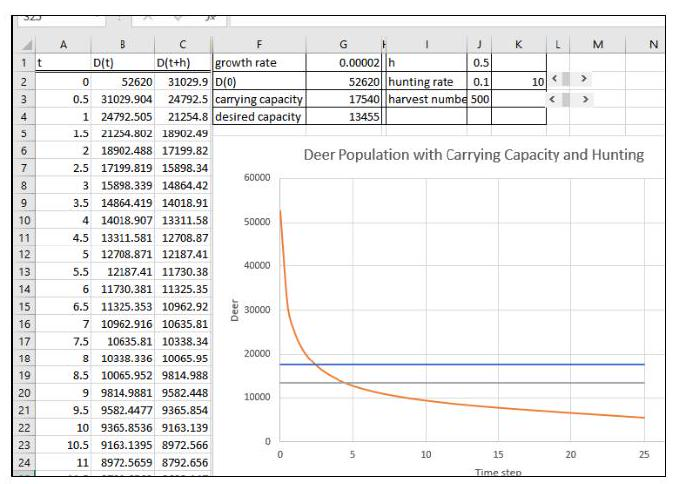
\includegraphics[max width=\textwidth]{2022_07_05_5945264bba2a5f6ba667g-13}

Another option is to use the Goal Seek function. Go to Data, then What-If-Analysis, then Goal Seek. If possible, Excel will find the solution. Note however that you can only use one variable at a time. A combination of hunting rate and harvest number is not possible. We will learn a method to deal with multivariable problems in the chapter on Simplex.

Assuming you want to reach the optimal density after 10 time steps by varying the hunting rate, then you will enter the information shown in the picture below. You will find that a $9.2 \%$ hunting rate is needed.

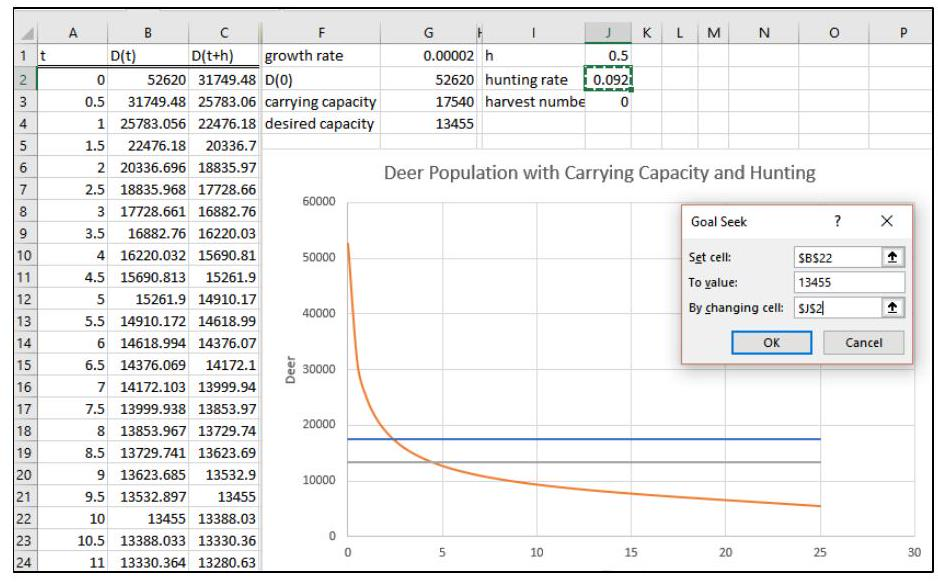
\includegraphics[max width=\textwidth]{2022_07_05_5945264bba2a5f6ba667g-14}

\section{Introducing Predators}
So far, we have investigated one population. Let's introduce a second population of predators, say coyotes. (While coyotes do rarely attack adult deer, they can kill up to $75 \%$ of newborn fawns). The population of deer should go up if there are many deer and few coyotes, and down if there are many coyotes and few deer. Similarly, the population of coyotes goes down if there are too many coyotes (starvation) and up if there are many deer. The two populations are mutually dependent. Of course, this is a bit of a simplification, as coyotes have other prey (rodents, hare, rabbits, carrion...)

Here is a possible model:

change in \# of deer = deer growth rate $\cdot \#$ of deer $-$ prey rate $\cdot \#$ of coyotes $\cdot \#$ of deer change in \# of coyotes = - coyote starvation rate $\#$ of coyotes $+$ feeding rate $\cdot$ \# of coyotes $\cdot \#$ of deer Here the "feeding rate" is really the rate at which deer are turned into baby coyotes.... Whenever you create a model, i.e. go from the real world to mathematical equations, you should make sure you define your variables and write down the definitions. Otherwise it will be almost impossible for anyone else - or you, later - to make sense of what you did. So, get into the habit.

Let $t=$ time
$$
\begin{aligned}
&D(t)=\text { number of deer at time } t \\
&C(t)=\text { number of coyotes at time } t \\
&r=\text { hamster growth rate } \\
&p=\text { prey rate } \\
&s=\text { starvation rate } \\
&f=\text { feeding rate }
\end{aligned}
$$
The model thus becomes a system of differential equations: $\quad D^{\prime}(t)=r \cdot D(t)-p \cdot C(t) \cdot D(t)$
$$
C^{\prime}(t)=-s \cdot C(t)+f \cdot C(t) \cdot D(t)
$$
I set this spreadsheet up a little different to make the formulas easier to read. Instead of computing $D(t+h)$ and $C(t+h)$ directly, we first compute the changes in $D(t)$ and $C(t)$, resp., and add them to (D(t) and $C(t) . D(t+h)$ thus becomes $D(t)+$ change in $D$, and $C(t+h)=C(t)+$ change in $C$.

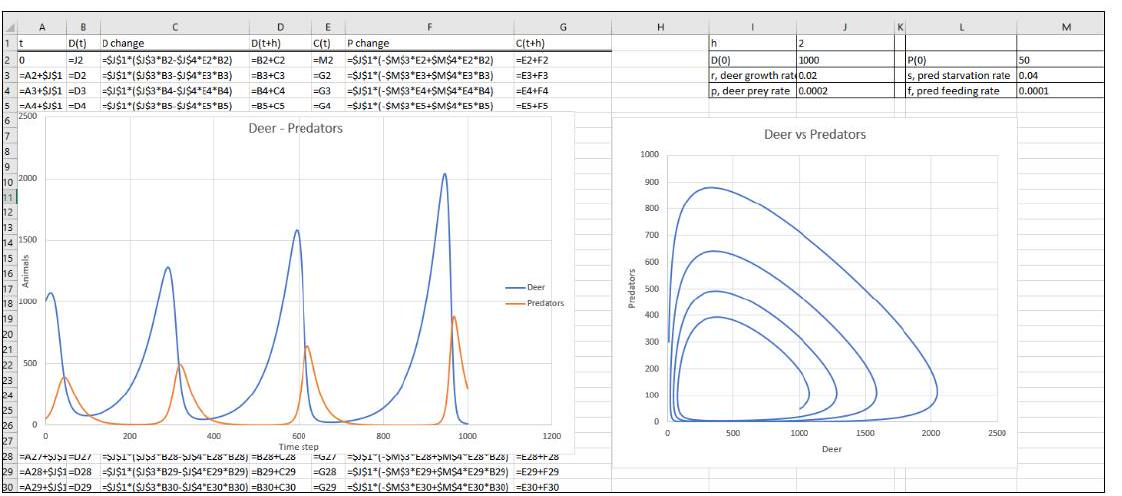
\includegraphics[max width=\textwidth]{2022_07_05_5945264bba2a5f6ba667g-15}

Have a look at the graph on the left. You see cyclical behavior in both populations, with the peaks increasing and slightly off-set. This is due to the time lag as a population increases due to increased food supply, or decreases due to lack of food and predation. This behavior becomes even more obvious as you plot deer population vs predators. Instead of reaching a constant state with seasonal fluctuations in populations, the coyote numbers will drop below 1, i.e. the predators will die out. Note: Any model is only as good as the data you used to construct it. Both the predator-prey model and the logistic growth model with hunting need to be carefully calibrated to make the model fit reality.

\section{Diagrams and Recursive Sequences - Multiple Populations}
Sometimes, it is more convenient or intuitive to express populations as recursive sequences. In that case, one would use $P_{0}$ instead of $P(0)$ and $P_{n}$ instead of $P(n h)$ or $P(t+h)$. For example, the logistic population model $P(t+h)=P(t)+h \cdot r \cdot P(t) \cdot(C-P(t))$ would become
$$
P_{n+1}=P_{n}+h \cdot r \cdot P_{n} \cdot\left(C-P_{n}\right), P_{0}=P(0) \text {. }
$$
In our current model, we really should consider more than two populations, even if we are concerned only with the deer population. Predators prey mostly on the young, only adults breed, and hunters will take only adults. When dealing with multiple populations, it often helps to represent to represent them with a diagram, where arrows represent the interactions between populations.

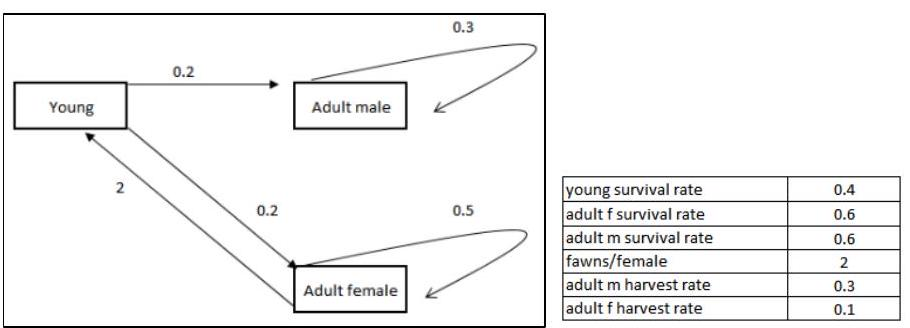
\includegraphics[max width=\textwidth]{2022_07_05_5945264bba2a5f6ba667g-16}

In this example, we assume that $40 \%$ of young grow up to be adults (half male, half female), each female produces 2 young per year, and the life span for adults is a little over two years. Male and female deer are hunted at different rates.

We express these relationships with recursive sequences:
$$
\begin{aligned}
&\mathrm{Y}_{\mathrm{n}+1}= \\
&\mathrm{F}_{\mathrm{n}+1}=0.2 \mathrm{Y}_{\mathrm{n}}+0.5 \mathrm{~F}_{\mathrm{n}} \\
&\mathrm{M}_{\mathrm{n}+1}=0.2 \mathrm{Y}_{\mathrm{n}}+\quad+0.3 \mathrm{M}_{\mathrm{n}}
\end{aligned}
$$
With $P_{n}:=\left[\begin{array}{c}Y_{n} \\ F_{n} \\ M_{n}\end{array}\right]$ and $A:=\left[\begin{array}{ccc}0 & 2 & 0 \\ 0.2 & 0.5 & 0 \\ 0.2 & 0 & 0.3\end{array}\right]$, this becomes $P_{n+1}=A \cdot P_{n}$.

If you took Linear Algebra with me, you may recognize this equation. However, the recurrence equations are easier to implement in Excel.

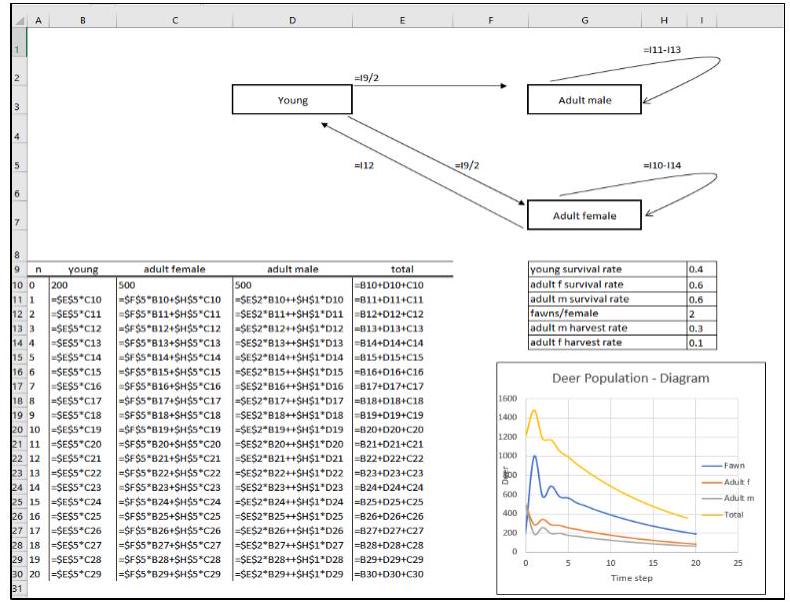
\includegraphics[max width=\textwidth]{2022_07_05_5945264bba2a5f6ba667g-17}

Obviously, the harvest rate here is too high; the population crashes. If you would outlaw doe hunting, the population stabilizes at 1378 total deer.

You may want to introduce additional refinements to your model, for example stocking or migration, a second food source, changing the constant growth rate to a seasonally varying rate, randomizing the prey rate, etc. At least at the beginning, while you are still getting used to this, it is important to start simple and slowly.

Note that this process can be used to model the spread of infections or rumors, a zombie apocalypse, chemical reactions, and more. This is a central concept of applied mathematics, adapting models and methods to the situation at hand.

\section{COMPUTING AREAS - SIMULATION 1}
\section{Learning Goals}
In this chapter, we will study how to estimate areas (integrals) using random numbers and repeated simulations. We will use Excel to

\begin{itemize}
  \item generate random numbers

  \item write simple IF statements

  \item use data tables for repeated simulations

\end{itemize}
\section{Case Study Description -Computing Areas}
Consider $\int_{a}^{b} \frac{1}{\sqrt{2 \pi} \sigma} e^{-\frac{(x-\mu)^{2}}{2 \cdot \sigma^{2}}} d x$. If you already took Statistics, you may recognize the Normal Distribution. More precisely, for a normally distributed random variable $x$ with mean $\mu$ and standard deviation $\sigma$ :
$$
P(a<x<b)=\int_{a}^{b} \frac{1}{\sqrt{2 \pi} \sigma} e^{-\frac{(x-\mu)^{2}}{2 \cdot \sigma^{2}}} d x .
$$
Unfortunately, this integral does not have a closed form solution (anti-derivative). Your task is to produce an EXCEL work sheet that approximates the value of the integral for any $a, b, \mu$, and $\sigma$ the user chooses

\section{Solution Approach}
There are many other and better solution approaches to this problem. We could use a series expansion such as Taylor series, or Riemann sums or Simpson's rule to approximate the value. However, the goal is to learn how to run simulations with EXCEL, so we will use that approach instead. The basic idea is to enclose the graph of the function in a rectangle and then generate many random points scattered uniformly across that rectangle. If you use enough points, and if you repeat the process often enough, then the ratio of the points under the curve to the total number of points should be equal to the proportion of the area under the curve. For example, if $90 \%$ of all random points end up under the curve, then it makes sense to assume that the area under the curve represents $90 \%$ of the total area. (Again, I realize this is not the most sensible approach, but we are focused on learning Excel here, not on finding the most elegant solution to a problem) The function $\frac{1}{\sqrt{2 \pi} \sigma} e^{-\frac{(x-\mu)^{2}}{2 \cdot \sigma^{2}}}$ takes on its maximum value at $\frac{1}{\sqrt{2 \pi} \sigma}$ and is always positive. It makes sense to use the rectangle from a to $b$ on the $x$-axis and from 0 to $\frac{1}{\sqrt{2 \pi} \sigma}$ on the $y$-axis.

To generate the random points, we use the rand() function. This function returns a random number between 0 and 1 . The $x$-coordinate of our point needs to be between a and $b$, so we need to stretch the interval $[0,1]$ by a factor of $a-b$ and shift by a factor of $a$. The $y$-coordinate of our point needs to be between 0 and $\frac{1}{\sqrt{2 \pi} \sigma}$, so we need to stretch the interval $[0,1]$ by a factor of $\frac{1}{\sqrt{2 \pi} \sigma}$. Next, we compute $y=f(x)=\frac{1}{\sqrt{2 \pi} \sigma} e^{-\frac{(x-\mu)^{2}}{2 \cdot \sigma^{2}}}$ to see if the point is below or above the curve. This is achieved with the IF statement: if the $y$-coordinate of the random point is less than $y=f(x)$, then we assign a value of 1 , else a value of 0 . We then have to add up all the " 1 "s and divide by the total number of random points used (I chose 500 ), to find the proportion of points under the curve. All that is left to do is to compute the area under the curve.

Here is what those formulas look like in Excel:

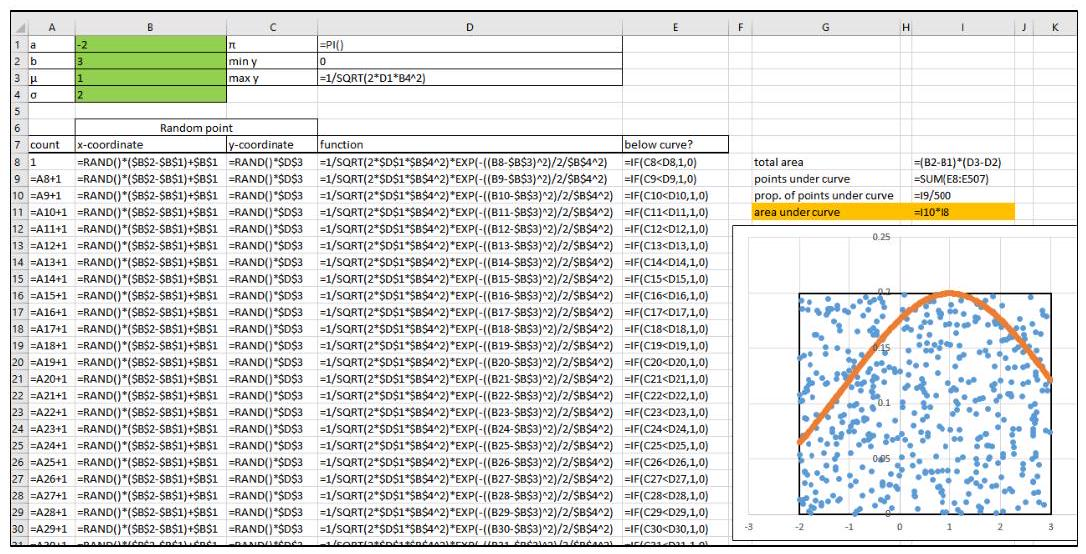
\includegraphics[max width=\textwidth]{2022_07_05_5945264bba2a5f6ba667g-19}

And here is a sheet showing some values:

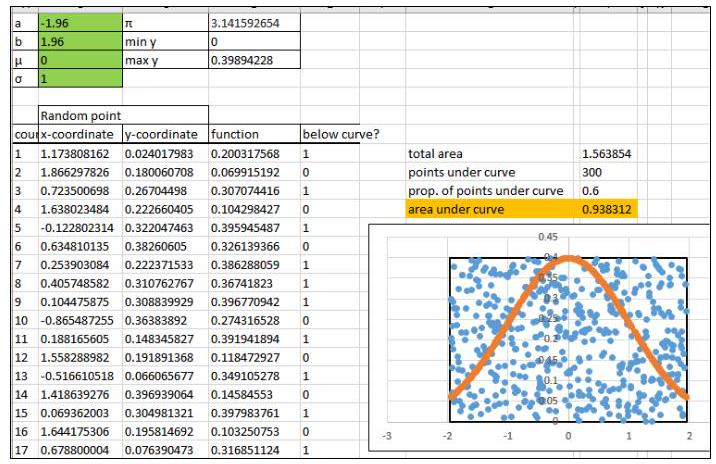
\includegraphics[max width=\textwidth]{2022_07_05_5945264bba2a5f6ba667g-20}

For $\mathrm{a}=-1.96, \mathrm{~b}=1.96, \mu=0$, and $\sigma=1$ the approximation exact to four decimals is $0.9500$, so we are a bit off. There are two ways to fix that. We could copy the formula to more than the 500 points used, or we could repeat the experiment many times and average the results. We will do the latter. Basically, we want to compute the area many, let's say 25 , times. To do that, first highlight where the table goes. It is important that the original computation is the top left cell, and that you have two columns. Next go to Data, What-If-Analysis, Data Table. Our table is arranged in a column, but because we do not want to change anything from run to run, we choose an empty unrelated cell as the Column input cell.

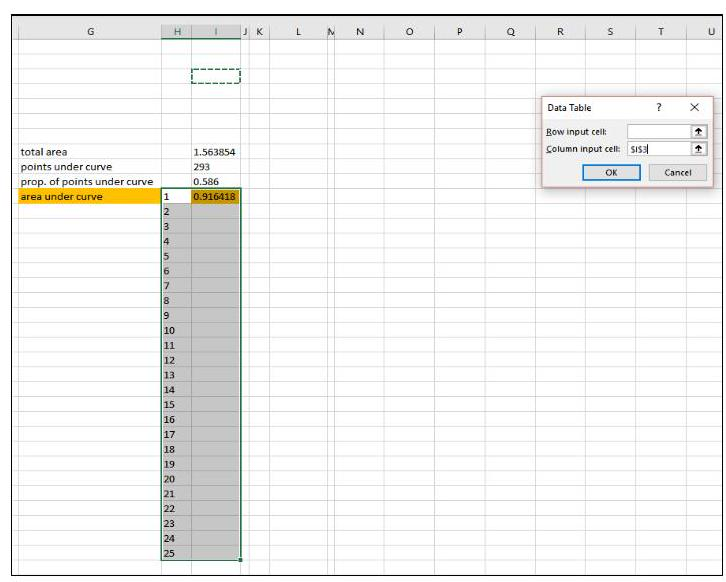
\includegraphics[max width=\textwidth]{2022_07_05_5945264bba2a5f6ba667g-20(1)}

Hit "enter, and you will see the results which you can then average with the "=AVERAGE(I11:|13)" command.

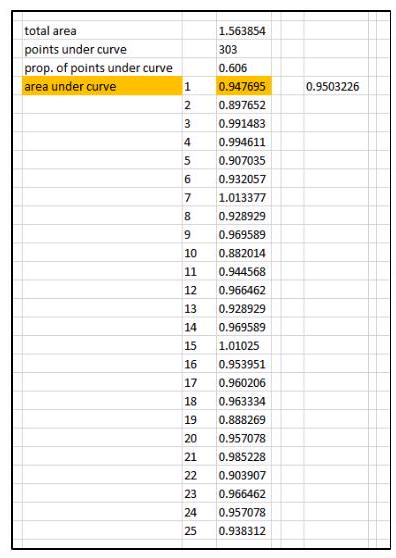
\includegraphics[max width=\textwidth]{2022_07_05_5945264bba2a5f6ba667g-21}

Note that this idea can be used to find the size of any area. You can use it to estimate constants, for example $\pi$. If you use a different distribution, you could model the spread of spills (normal distribution), population density of bugs (Poisson distribution), and more. Modeling is all about being creative, using methods and ideas you may be familiar with and then adapting them to new situations.

\section{MODELING THE SPREAD OF DISEASES - SIMULATION 2}
\section{Learning Goals}
After this chapter, you, you should be able to:

\begin{itemize}
  \item Use nested IF, AND statements

  \item Use COUNTIF

  \item Use RANDBETWEEN

  \item Record macros

  \item Use conditional formatting

\end{itemize}
\section{Case Study Description - Diseases}
An outbreak of a new flu strain needs to be contained. For this particular flu, people will get sick only if they have contact with one or more sick people, and then only with a $50 \%$ chance. Once sick, they either recover and become immune, or they die. The probability of dying increases with the number of sick people the patient came in contact with while being sick: 0 contacts: full recovery and immunity, 1 -4 contacts, $5 \%$ chance of death, 5-9 contacts, $20 \%$ chance of death. Generate a spreadsheet that simulates the spread of disease through a population.

\section{Solution Approach}
There are many - and better - ways to model the spread of diseases than the following. However, the point is to learn how to use the nested "if" statement, conditional formatting, and macros, so bear with me.

A problem like this becomes messy fast, so we will start simple and then refine. A flow chart helps to organize and then simplify all the rules. To deal with probabilities, imagine flipping a coin or die.

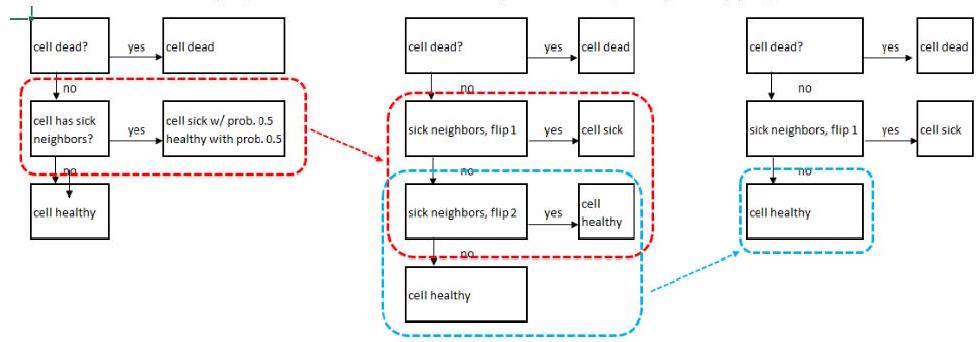
\includegraphics[max width=\textwidth]{2022_07_05_5945264bba2a5f6ba667g-22}

Syntax: $\quad=\operatorname{IF}$ (Statement to check, what to do/value if true, what to do/value if false)

AND (statement 1, statement 2,..)

$=$ COUNTIF (range, when to count)

=RANDBETWEEN (lower bound, upper bound)

In this case: $=\mathrm{IF}($ cell is dead, dead, IF(AND(cell has $1+$ sick neighbors, flip 1), sick, healthy)))

We will use three $25 \times 25$ grids: one represents the state today, one the state tomorrow, and one keeps track of the number of sick neighbors each cell has. We assign an arbitrary value to the four possible states, dead $=0$, sick $=1$, healthy $=2$, immune $=3$.

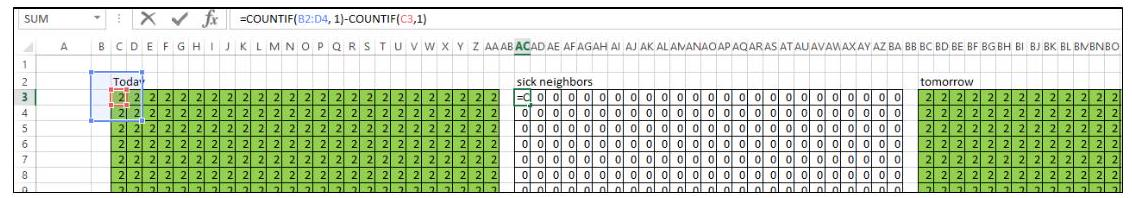
\includegraphics[max width=\textwidth]{2022_07_05_5945264bba2a5f6ba667g-23}

Below is a screenshot of the formula you need to enter in the "tomorrow" block and copy to all cells in that block.

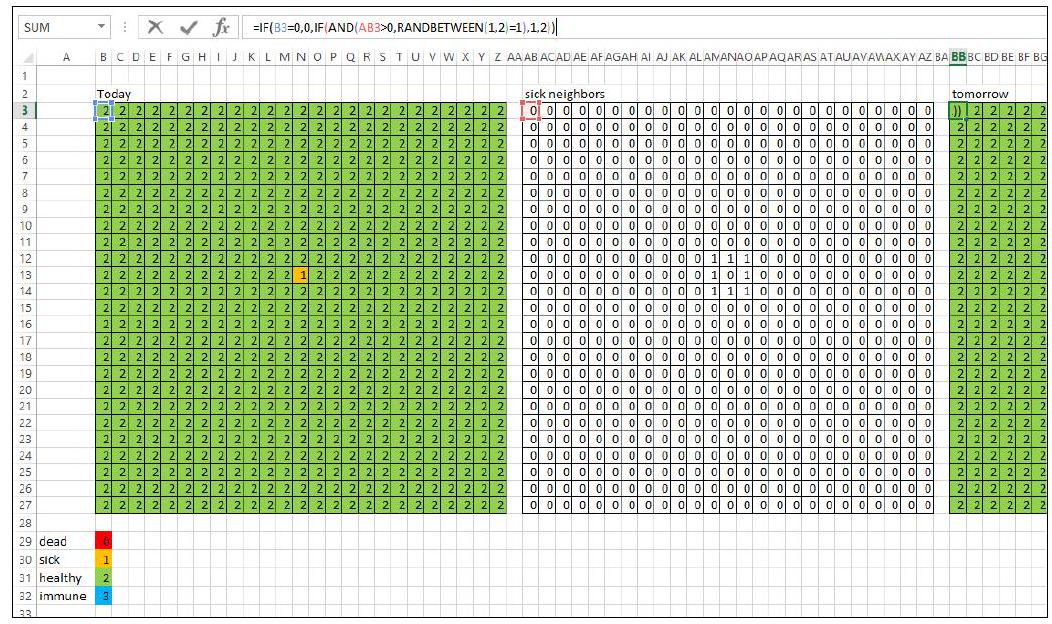
\includegraphics[max width=\textwidth]{2022_07_05_5945264bba2a5f6ba667g-23(1)}

Pretty up your worksheet by adding titles and conditional formatting to the blocks. Conditional formatting is under the HOME tab.

Including all the rules give a flow chart like this:\\

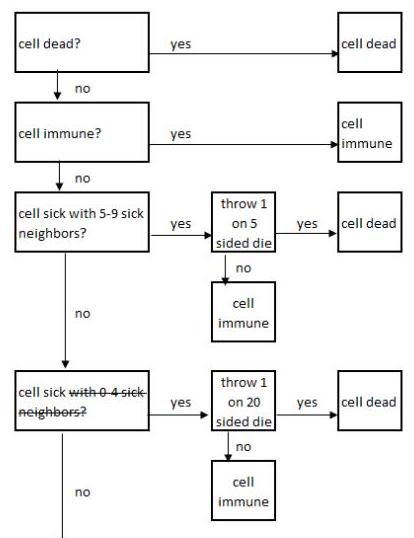
\includegraphics[max width=\textwidth]{2022_07_05_5945264bba2a5f6ba667g-24}

Note: We do not need to include the sick neighbors here. We already know it does not have $5-9$ sick neighbors, so $0-4$ is the only option left

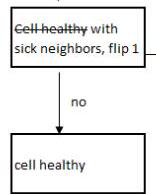
\includegraphics[max width=\textwidth]{2022_07_05_5945264bba2a5f6ba667g-24(1)}

Note: We do not need to include that the cell is healthy, because that is the only possibility left at this point

This gives a very convoluted nested statement, give it a shot yourself before you look up the solution. Add a few formulas that count the number of sick, healthy, immune, and dead cells.

Finally, we include macros. When you record a macro, you really create a short cut to perform a series of tasks. You use it if you need to repeat those tasks repeatedly. Basically, you replace a series of key strokes or instructions with a single keystroke. We record two macros, one to copy the values of the third (tomorrow) block to the first (today) block, and one to re-set the whole worksheet. The record macro button is in the DEVELOPER tab. Make sure to remember to add a description of your macro.

As you run your worksheet, if you start with a single sick cell in the center, you should see an everexpanding blob of dead and immune cells and a few healthy ones. Because of the randomness involved, and depending on your styling, your sheet will look different than mine.

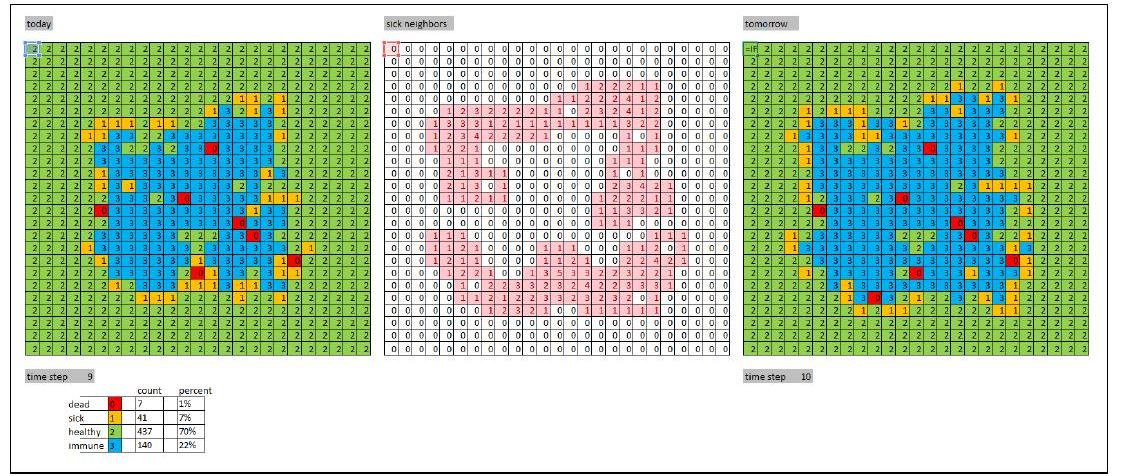
\includegraphics[max width=\textwidth]{2022_07_05_5945264bba2a5f6ba667g-25}

And here is a solution for the formula that goes into the tomorrow block (cell BC4 is the top left cell for me) and then is copied to all the cells in the block:\\

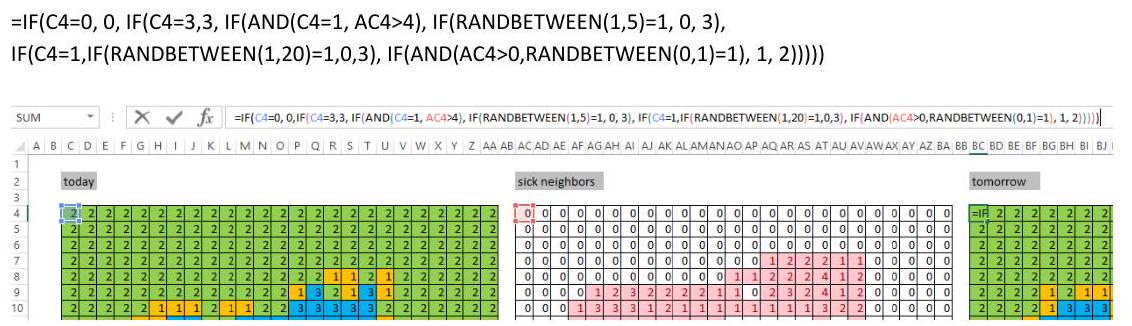
\includegraphics[max width=\textwidth]{2022_07_05_5945264bba2a5f6ba667g-25(1)}

This set up can be used to model anything where the state of one cell depends on some or all of its neighbors. Applications include: spread of rumors, dissipation of heat, spread of a population, Zombies invading, built-up in cities, invasive species, ...

\chapter{CASE STUDY - Designing a campground - Simplex method}
\todoChapter{ 0\% complete. \\
Notes: Borrowed from Karin Vorwerk.  Need to integrate this into other chapters.}
\section{DESIGNING A CAMPGROUND - SIMPLEX METHOD}
The Simplex method is probably the classic method of solving constraint optimization problems. We will use this solution approach, sometimes in modified form, over and over in this class, not just in this chapter.

\begin{outcome}
You will learn

\begin{itemize}
  \item How to recognize linear programming (LP) problems

  \item Vocabulary of LP problems

  \item Graphical solution

  \item Algebraic solution

  \item Excel solution with the Excel Solver

\end{itemize}
\end{outcome}
\subsection{Case Study Description - Campground}
You are opening a campground in the Florida Keys, and you are trying to make as much money as possible. You are planning a mix of RV sites, tent sites, and yurts. Let's assume you already own 10 acres, and that you can make $\$ 80 /$ day profit on each $\mathrm{RV}, \$ 20 /$ day profit on each tent, and $\$ 200$ profit on each Yurt. However, there are restrictions:

\begin{enumerate}
  \item Infrastructure takes up $20 \%$ of your site

  \item You can have 20 RVs per acre, or

  \item You can have 40 tents per acre, or

  \item You can have 10 yurts per acre

  \item You have a budget of $\$ 100,000$. It costs you $\$ 1000$ to develop an $R V$ site, $\$ 200$ for a tent site, and $\$ 8000$ for a yurt.

  \item Maintenance for the bath houses etc. is $15 \mathrm{~min} /$ week/camper unit. You can afford 70hrs/week in maintenance help

  \item Zoning ordinance requires you to have at least 20 tent sites What is the best layout for your campground, and how much profit can you make per day?

\end{enumerate}
\subsection{References}
This case study was inspired by the Knights Key RV park in Florida. Read more about it here: \href{http://www.knightskeyrvresortandmarina.com/news/}{http://www.knightskeyrvresortandmarina.com/news/} \href{http://www.miaminewtimes.com/news/developers-plan-to-replace-rv-park-with-fivestar-resort-stirs-fears-hopes-in-keys-8038648}{http://www.miaminewtimes.com/news/developers-plan-to-replace-rv-park-with-fivestar-resort-stirs-fears-hopes-in-keys-8038648}

\subsection{Solution Approach - Two Variables}
We will again first look at a simpler problem by ignoring the yurts and only considering RV spaces and tents.

Let $r$ be the number of RVs, $t$ the number of tents, and $P(r, t)$ the profit. Your goal is to maximize $P(r, t)=$ $80 \mathrm{r}+20 \mathrm{t}$. This function is called the objective function. The variables $r$ and $t$ are called decision

variables. You can see that in the current case $P(r, t)$ gets bigger if you increase $r$ and/or $t$. If you picture a graph with $r$ on the horizontal and $t$ on the vertical axis, then the direction of increase for the objective function is to the top right.

Translating the relevant restrictions into equations gives

\begin{enumerate}
  \item $r / 20+t / 40 \leq 8$

  \item $r \leq 160$

  \item $t \leq 320$

  \item $(r+t) / 4 \leq 70$

  \item $t \geq 20$

  \item $r, t \geq 0$

  \item $1,000 r+200 t \leq 100,000$

\end{enumerate}
Simplified

\begin{enumerate}
  \item $2 r+t \leq 320$

  \item $r \leq 160$

  \item $t \leq 320$

  \item $5 r+t \leq 500$

  \item $r+t \leq 280$

  \item $\mathrm{t} \geq 20$

  \item $r, t \geq 0$

\end{enumerate}
These are called the functional constraints.

In addition, you can't have negative sites, so we have the non-negativity constraints

\begin{enumerate}
  \setcounter{enumi}{5}
  \item $r \geq 0$

  \item $t \geq 0$.

\end{enumerate}
A problem like the above with linear constraints and a linear objective function is called a linear programming problem.

\subsection{Assumptions made about linear programming problem}
\paragraph{Proportionality} For both the objective function and the constraints, a change in a decision variable will result in a proportional change in the objective function or constraint. (Note that this rules out any exponents on the decision variables other than 1.)

\paragraph{Additivity} Both the objective function and the constraints are the sums of the respective changes in the decision variables (This means no multiplying different decision variables).

Basically, the proportionality and additivity assumptions are just fancy ways of saying that all functions in a linear programming problem are linear in the decision variables.

\paragraph{Divisibility} We are assuming that our decision variables can be non-integer, i.e. may take on fractional values. Problems with an integer constraint are called integer programming problems, we will only touch on them briefly later. Certainty We act as if the value assigned to each parameter is known, precise, and constant over time. This is rarely the case, so we need to compensate for that by performing sensitivity analysis. Basically, we need to investigate how much it affects our solution if the parameters change.

\subsection{Graphical Simplex solution procedure}
We will start with some vocabulary:

\begin{itemize}
  \item Feasible solution: A solution for which all constraints are satisfied, not necessarily an optimal Solution.

  \item Infeasible solution: A solution that violates at least one constraint.

  \item Optimal solution: a solution that optimizes (could be a minimum or maximum, depending on your problem) the objective function. There may or may not be an optimal solution.

\end{itemize}
Feasible region: The set of all feasible solutions

\begin{itemize}
  \item Corner point: the intersection of two or more constraints

  \item Corner point feasible solution CPF solution: A solution that occurs at a corner of the feasible region

\end{itemize}
The first step in the graphical solution procedure is to draw the feasible region (note that this gets really ugly if you have three or more variables).

The non-negativity constraints mean that we are looking for a solution in the first quadrant only. The constraints 2) $r \leq 160,3) t \leq 320$, and 7) $t \geq 20$ mean you have to stay left of the line $r=160$, below the line $t=320$ and above the line $t=20$. You see that the constraint $t \geq 20$ dominates the constraint $t \geq 0$, so the latter is redundant.

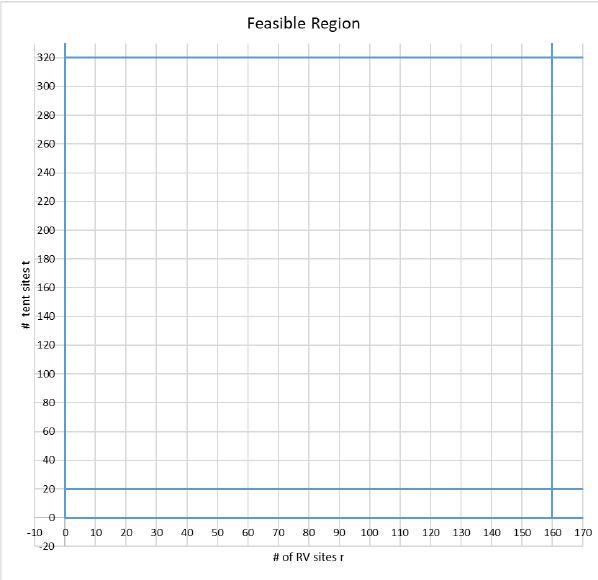
\includegraphics[scale = 0.35]{2022_07_05_5945264bba2a5f6ba667g-28}

Adding the remaining constraints yields this graph: Go ahead, shade the feasible region and identify all redundant constraints.

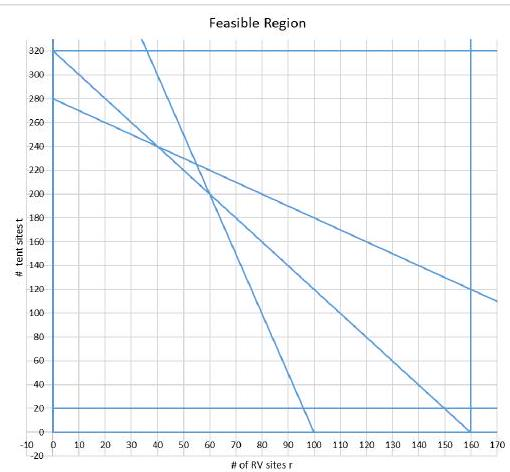
\includegraphics[scale = 0.5]{2022_07_05_5945264bba2a5f6ba667g-29}

All the points in the feasible region are possible solutions. Your job is to pick (one of) the best solutions. Note that there may not be a single best solution but rather several optimal solutions.

We have not yet used the objective function $P(r, t)=80 r+20 t$. Because we do not have a value for $P(r, t)$, so we will draw $P(r, t)$ for a few random values of $P(r, t)$ to get an idea of what it looks like. For $P(r, t)=1600,2400,3200$ we get the lines shown in the next picture. Note that they are all parallel, and that the lines corresponding to the larger value of $P(r, t)$ move to the top left. The direction of increase is just as we expected, to the top right.

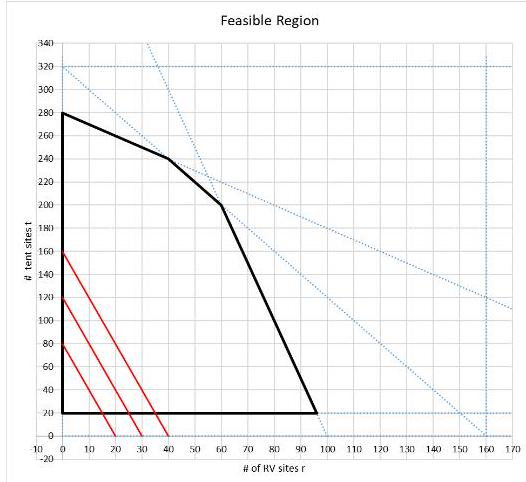
\includegraphics[scale = 0.5]{2022_07_05_5945264bba2a5f6ba667g-29(1)}

As you move the line for the $P(r, t)$ to the right you increase your profit. But you also have to stay in the feasible region. Convince yourself that one of two cases will occur: either a unique optimal solution will be found at a corner point, or infinitely many optimal solutions returning the same maximum value for $P(r, t)$ will be found along a section of the boundary of the feasible region that includes two corner points. Therefore, we need to compute the corner points, i.e. the intersections of the constraints, and move $P(r, t)$ as far to the right as possible without leaving the feasible region.

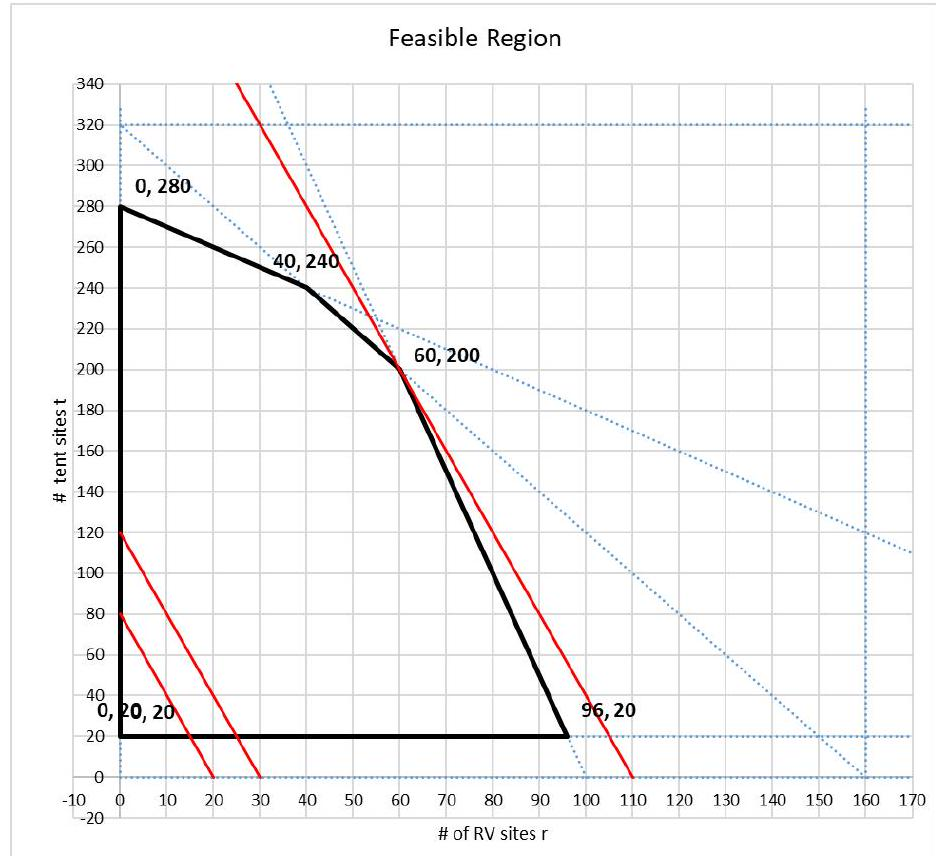
\includegraphics[scale = 0.3]{2022_07_05_5945264bba2a5f6ba667g-30}

From the picture above, you can see that the optimal solution will be at the intersection of the lines corresponding to constraints 1) and 5).
$$
r / 20+t / 40 \leq 8 \text { and } 1000 t+200 t \leq 100,000
$$
which is at the point $r=60, t=200$. (Now would be a good time to review how to solve systems of equations....). This gives us a profit $P(60,200)=60 \cdot \$ 80+200 \cdot \$ 20=\$ 8800$.

\subsection{Stating the Solution}
In OR, typically someone hires you to work your problem, and then expects you to give the answer in the context of the problem. You can't just say "the solution is at $r=60, t=200, P(r, t)=8800$ ". Give the answer like this:

"To maximize potential profit, the campground should have $60 \mathrm{RV}$ sites and 200 tent sites. In that case, the potential profit per day, assuming full occupancy, is $\$ 8800$. You are limited by the available land and budget available, not by available labor or any zoning rules. You will have to hire 65 hours of help per week (260 camping units at 15 minutes/week/unit)."

\subsection{Refinements to the graphical solution}
One "brute force" approach to the graphical solution method would be to compute all intersections of all constraints, check if that corner is in the feasible region, and then compute the objective function at those points. However, the number of intersections increases quadratically with the number of lines ( $\frac{\mathrm{n}(\mathrm{n}+1)}{2}$ for $n$ non-parallel lines), so this approach quickly gets out of hand. Instead, the idea is to start at an easy to find corner of the feasible region. Often, the origin works. From that point, check the adjacent feasible corner points and move to the "best". Continue until there is no more improvement. Here is what that would look like in our case:

We start at a simple corner. Usually, people use the origin, which is not on the feasible region here, so we start at $(0,20)$. Adjacent corners are $(0,280)$ and $(96,20)$ with $P(0,20)=400, P(0,280)=5600$, and $P(96,20)=8080$. $(96,20)$ is best, so we move there. Next, check the adjacent corner $(60,200)$. It gives $P(60,200)=8800$ which is an improvement, so move there. Check the next adjacent corner $(40,240)$ It gives $P(40,240)=8000$. This is worse, so $(60,200)$ is the optimal solution.\\

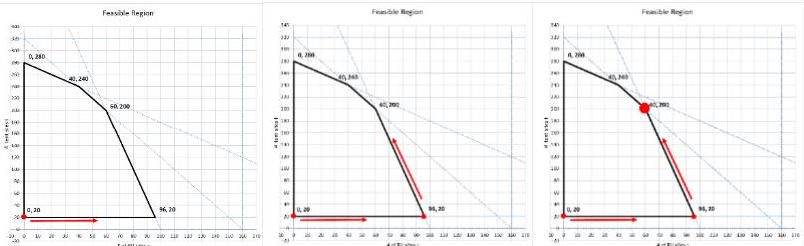
\includegraphics[scale = 0.5]{2022_07_05_5945264bba2a5f6ba667g-31}

There is of course a big problem with this approach. It relies on us having a graph of the feasible region and being able to see the adjacent feasible corner points. If you are dealing with a large number of constraints and variables, this is not possible. We therefor take the idea of looking at adjacent feasible corners and moving towards the one that gives the best value for the objective function, and translate it into an algebraic method.

\paragraph{Solution Approach - Algebraic Simplex Method}
As these are only three variables, we could still draw the feasible region, now a solid bound by planes. However, we need an approach that works for any number of variables. The key to this method is the fact that an optimal solution will occur at a corner point of the feasible region. While the n-dimensional proof is beyond the scope of this class, this fact should be intuitively clear in the 2-d and 3-d cases.

We will first demonstrate the algebraic method on the two-variable problem (RV and tent only) and then solve the full problem.

\paragraph{Corner points, interior corner points, slack variables}
We introduce slack variables to turn the inequalities into equalities. Basically, a slack variable lets you know how close you are to maxing out the constraint. In the current case, we have:

\begin{tabular}{ll}
Constraints &
Augmented constraints\\
1) $4 r+t \leq 320$ &
1) $2 r+t+s_{1}=320$\\
2) $5 r+t \leq 500$&
2) $5 r+t+s_{2}=500$\\
3) $r+t \leq 280$&
3) $r+t+s_{3}=280$\\
4) $t \geq 20$&
4) $\mathrm{t}-\mathrm{s}_{4}=20$\\
5) $r, t \geq 0$&
5) $r, t, s_{1}, s_{2}, s_{3}, s_{4} \geq 0$
\end{tabular}

A point is a corner point if it sits at the intersection of two or more constraints, i.e. if two or more slack variables are zero. A point is a feasible solution (i.e. inside the feasible region) if all slack variables are non-negative. A point is outside the feasible region if any slack variable is negative. We will from now on express each point as $\left(r, t, s_{1}, s_{2}, s_{3}, s_{4}\right)$. Given $r$ and $t$, one computes the values of the slack variables from the augmented constraints.

$\begin{array}{lllll}\text { Examples: } & r=100, t=20 \quad \rightarrow \quad(100,20,100,-20,140,0) & \text { outside the feasible region } \\ & r=10, t=30 \quad & \rightarrow & (10,30,270,420,240,10) & \text { inside feasible region } \\ r=150, t=20 & \rightarrow & (150,20,0,-270,110,0) & \text { corner outside feasible region }\end{array}$

\paragraph{Initializing}
Because $(0,0)$ is not on the feasible region, we again start at $(r, t)=(0,20)$, which has the augmented form $(0,20,300,480,240,0)$. We are sitting on the intersection of the lines $r=0$ and $t=20$.

\paragraph{The adjusted objective function}
Note: If the origin is a feasible corner point and you start at the origin, you can skip this step.

We are sitting on the intersection of the lines $r=0$ and $t=20$. To reach the next adjacent corner, we have to move along one of those lines, but which one? If we move along the line $r=0$, we move away from the line $t=20$, which is the same as saying we are increasing the corresponding slack, $s_{4}$. If we move along the line $t=20$, we increase $r$. We want to choose the direction of increase that gives us the fastest increase in $P$. The original objective function is $P(r, t)=80 r+20 t$, which does not let us see what happens if we increase $s_{4}$ We have to rewrite $P(r, t)$ in terms of $r$ and $s_{4}$.

Using equation 4) we get $t=20+s_{4}$, and thus $P\left(r, s_{4}\right)=80 r+20\left(20+s_{4}\right)=400+80 r+20 s_{4}$

\subsection*{Determining which way to move}
We want to choose the direction of increase that gives us the fastest increase in P. The objective function is $P\left(r, s_{4}\right)=400+80 r+20 s_{4}$. Because the variable $r$ has the biggest coefficient, 80 , an increase in r should give the best return.

\subsection*{Determining how far to move - the next corner}
We will leave $s_{4}$ at is current value, 0 , and increase $r$ as much as possible without leaving the feasible region, i.e. without having $t, s_{1}, s_{2}, s_{3}, s_{4}$ become negative.

\begin{enumerate}
  \item $2 r+t+s_{1}=320$\\
$s_{1}=320-20-2 r \geq 0$, so $r \leq 150$\\
$s_{2}=500-20-5 r \geq 0$, so $r \leq 96$
  \item $5 r+t+s_{2}=500$\\
$S_{3}=280-20-r \geq 0$, so $r \leq 240$
  \item $r+t+s_{3}=280$
  \item $t-S_{4}=20$\\
$t=20$
\end{enumerate}
So, $r$ can be increased to 96 .

\subsection*{Augmented form of the next corner}
Using $r=96, s_{4}=0$, and substituting into the equations $1-4$, we have the augmented point $(96,20,108,0$, $164,0)$. Note that this is the same corner $(96,20)$ we used above.

\subsection*{The adjusted objective function}
We are now sitting on the intersection of the lines $5 r+t+s_{2}=500$ and $t=20$. To reach the next adjacent corner, we have to move along one of those lines, which means either increasing $s_{2}$ or $s_{4}$. We have to rewrite $P(r, t)$ in terms of $s_{2}$ and $s_{4}$.

Using equations 2 and 4 , we find that $5 r=500-t-s_{2}$ and $t=20+s_{4}$, which yields $5 r=480-s_{4}-s_{2}$. Substituting into $P$ :

$P\left(s_{2}, s_{4}\right)=400+80 r+20 s_{4}=400+16\left(480-s_{4}-s_{2}\right)=20 s_{4}=8080+4 s_{4}-16 s_{2}$

Now we will repeat the above steps until the solution/objective function can no longer be improved upon.

\paragraph{Determining which way to move}
Because the $\mathrm{S}_{4}$ has the only positive coefficient, this is the only direction that will yield an increase in $\mathrm{P}$.

\paragraph{Determining how far to move - the next corner}
We will leave $s_{2}$ at is current value, 0 , and increase $s_{4}$ as much as possible without leaving the feasible region.

\begin{enumerate}
  \item $2 r+t+s_{1}=320 \quad s_{1}=320-t-2 r$
  \item $5 r+t+s_{2}=500$\\
$\mathrm{s}_{2}=500-\mathrm{t}-5 \mathrm{r}$
  \item $r+t+s_{3}=280$\\
$\mathrm{s}_{3}=280-\mathrm{t}-\mathrm{r}$
  \item $t-s_{4}=20$ $\mathrm{t}=20+\mathrm{s}_{4}$
\end{enumerate}
We use that $s_{2}=0$ and $t=20+s_{4}$. This gives the set of equations:

\begin{enumerate}
  \item $s_{1}=108-0.6 s_{4}$\\
$\geq 0$, so $\mathrm{s}_{4} \leq 96$\\
$\geq 0$, so $\mathrm{S}_{4} \leq 480$

  \item $r=96-0.2 s_{4}$\\
$\geq 0$, so $\mathrm{S}_{4} \leq 205$

  \item $\mathrm{s}_{3}=164-0.8 \mathrm{~s}_{4}$

  \item $t=20+s_{4}$

\end{enumerate}
$\geq 0$, so $\mathrm{s}_{4} \geq-20$ (as 20 is positive, this is true anyway) So $\mathrm{S}_{4}$ can be increase up to 180 .

\paragraph{Augmented form of the next corner}
Using $s_{2}=0, s_{4}=180$, and substituting into the equations $1-4$, we have the augmented point $(60,200,0,0$, $20,180)$. Note that this is the second corner $(60,200)$ we used above.

\paragraph{The adjusted objective function}
We again re-write the objective function, this time in terms of $s_{1}$ and $s_{2}$ : $P\left(s_{1}, s_{2}\right)=8080+4 s_{4}-16 s_{2}=8080+4\left(180-1.6 s_{1}\right)-16 s_{2}=8800-6.6 s_{1}-16 s_{2}$. Note that increasing either $s_{1}$ or $s_{2}$ will decrease the value of $P$, so we have reached the maximum. As $s_{1}$ and $s_{2}$ are non-negative, we can also see that the maximum for $P$ occurs when $s_{1}$ and $s_{2}$ are zero, at $P=8800$. Again, this is the same answer we arrived at earlier.

A nice side effect is that we can tell which constraints are holding us back, namely those associated with the zero slack variables $s_{1}$ and $s_{2} . s_{1}$ corresponds to the space limitations, and $s_{2}$ to the budget restrictions.

\subsection*{Solving the full problem}
We are now ready to look at the original problem. We will assume you went to the bank and got a loan for $\$ 246,000$ to supplement your original budget. Here are the constraints again:

\begin{enumerate}
  \item Infrastructure takes up $20 \%$ of your site

  \item You can have $20 \mathrm{RV}$ s per acre, or

  \item You can have 40 tents per acre, or

  \item You can have 10 yurts per acre

  \item You have a budget of $\$ 346,000$. It costs you $\$ 1000$ to develop an RV site, $\$ 200$ for a tent site, and $\$ 8000$ for a yurt.

  \item Maintenance for the bath houses etc. is $15 \mathrm{~min} /$ week/camper unit, you can afford $70 \mathrm{hrs} /$ week in maintenance help

  \item Zoning ordinance requires you to have at least 20 tent sites

\end{enumerate}
\begin{tabular}{|l|l|l|}
\hline
Functional Constraints & $\underline{\text { Simplified Constraints }}$ & $\underline{\text { Augmented Constraints }}$ \\
\hline
$\mathrm{r} / 20+\mathrm{t} / 40+\mathrm{y} / 10 \leq 8$ & $2 \mathrm{r}+\mathrm{t}+4 \mathrm{y} \leq 320$ & $2 \mathrm{r}+\mathrm{t}+4 \mathrm{y}+\mathrm{s}_{1}=320$ \\
$1000 \mathrm{r}+200 \mathrm{t}+8000 \mathrm{y} \leq 346,000$ & $5 r+t+40 \mathrm{y} \leq 1730$ & $5 \mathrm{r}+\mathrm{t}+40 \mathrm{y}+\mathrm{s}_{2}=1750$ \\
$(\mathrm{r}+\mathrm{t}+\mathrm{y}) / 4 \leq 70$ & $\mathrm{r}+\mathrm{t}+\mathrm{y} \leq 280$ & $\mathrm{r}+\mathrm{t}+\mathrm{y}+\mathrm{s}_{3}=280$ \\
$\mathrm{t} \geq 20$ & $\mathrm{t} \geq 20$ & $\mathrm{t}-\mathrm{s}_{4}=20$ \\
\hline
\end{tabular}

\paragraph{Non-negativity constraints:}
$r, t, y_{1}, s_{1}, s_{2}, s_{3}, s_{4} \geq 0$

\paragraph{Objective function:}
Maximize $P(r, t, y)=80 r+20 t+200 y$

\paragraph{Initializing}
Because $(0,0,0)$ is not on the feasible region, we start at $(r, t, y)=(0,20,0)$, which has the augmented form $(0,20,0,300,480,240,0)$. We are sitting on the intersection of the planes $r=0, t=20, y=0$. The augmented form of this corner is $(0,20,0,300,1710,260,0)$

\paragraph{The adjusted objective function}
Rewriting $P$ as $P\left(r, y, s_{4}\right)$ gives: $P\left(P\left(r, y, s_{4}\right)=400+80 r+200 y+20 s_{4}\right.$

\paragraph{Determining which way to move}
Looking at the coefficients of $r, y, s_{4}$ in the objective function, we find that we should increase $y$ and leave $r$ and $s_{4}=0$

\paragraph{Determining how far to move - the next corner}
Using $r=0$ and $s_{4}=0$, the constraints become

$\begin{array}{lllll}t+4 y+s_{1}=320 & 4 y+s_{1}=300 & s_{1}=300-4 y & \geq 0 & \rightarrow y \leq 75 \\ t+40 y+s_{2}=1750 & 40 y+s_{2}=1730 & s_{2}=1730-40 y & \geq 0 & \rightarrow y \leq 42.75 \\ t+y+s_{3}=280 & y+s_{3}=260 & s_{3}=260-y & \geq 0 & \rightarrow y \leq 260\end{array}$

$t=20$

So, y can be increased up to $42.75$

\paragraph{Augmented form of the next corner}
With $\mathrm{r}=0, \mathrm{~s}_{4}=0$, and $\mathrm{y}=42.75$, we find the new augmented corner to be $(0,20,42.75,129,0,217.25,0)$.

\paragraph{The adjusted objective function}
We need to rewrite the objective function in terms of $r, s_{2}$, and $s_{4}$ :

$P\left(r, s_{2}, s_{4}\right)=8950+55 r+15 s_{4}-5 s_{2}$

The solution is not optimal yet, (there are still positive coefficients in the objective function), so we keep going.

\paragraph{Determining which way to move}
We see that we should increase $r$ and leave $s_{2}$ and $s_{4}=0$.

Determining how far to move - the next corner

With $s_{2}$ and $s_{4}=0$, we have

$\begin{array}{llll}2 r+t+4 y+s_{1}=320 & 2 r+4 y+s_{1}=300 & s_{1}=129-1.5 r \geq 0 & \rightarrow r \leq 86 \\ 5 r+t+40 y=1750 & 5 r+40 y=1730 & 40 y=1710-5 r & \\ r+t+y+s_{3}=280 & r+y+s_{3}=260 & s_{3}=236.25-0.875 r \geq 0 & \rightarrow r \leq 342\end{array}$

$t=20$

So, y can be increased up to 86

\paragraph{Augmented form of the next corner}
With $y=86, s_{2}=2$, and $s_{4}=0$ we find the new augmented corner to be $(86,20,32,0,0,142,0)$

\paragraph{The adjusted objective function}
We need to rewrite the objective function in terms of $s_{1}, s_{2}$, and $s_{4}$ :

$P\left(s_{1}, s_{2}, s_{4}\right)=13680-36 \frac{2}{3} s_{1}-1 \frac{1}{3} s_{2}-18 s_{4}$

Note that now all variables have negative coefficients, so we cannot increase the value of P past 13680. The first, second, and fourth constraints are maxed out; we are limited in our ability to increase the profit by space, money, and zoning restrictions.

\subsection*{ Stating the Solution }
To maximize potential profit, the campground should have 86 RV sites, 20 tent sites, and 32 yurts. This will take an initial investment of $\$ 346,000$. The potential profit per day, assuming full occupancy, is $\$ 13,680$. You are limited by the available land and budget available and the zoning law requiring 20 tent sites. You will have to hire $34.5$ hours of help per week (138 camping units at 15 minutes/week/unit)."

\subsection{Solution Approach - Using Excel}
Now that we know how the solution method works, we can use Excel to do the work for us. First, we must set up the work sheet. One way that works well is shown on the next page. The fields highlighted in green are necessary, the others serve to explain and label what we are doing.

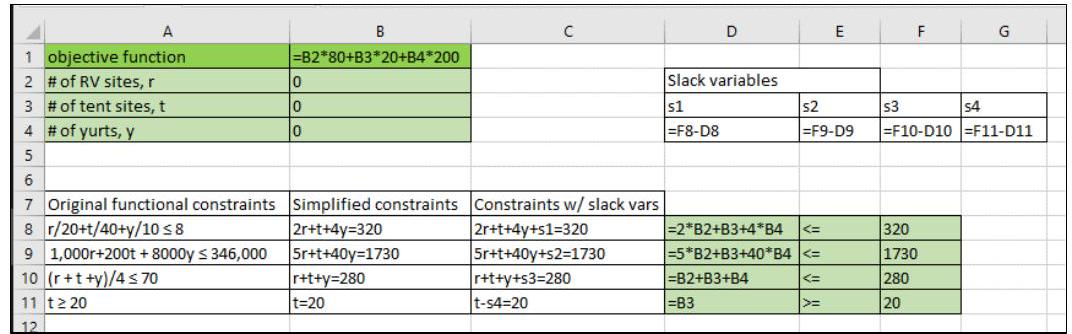
\includegraphics[scale = 0.5]{2022_07_05_5945264bba2a5f6ba667g-37}

Excel has a built-in Solver under the Data tab (if you don't see it, you have to add it in. Go to file/options/Add-ins/Manage Excel Add-ins/Solver Add-in). If you choose "show iteration results in the options tab, the solver will stop at each iteration and show you the corner/solution it has arrived found at that step. You will see that the solver goes through the same steps and corner points as we did when we worked the problem "by hand".

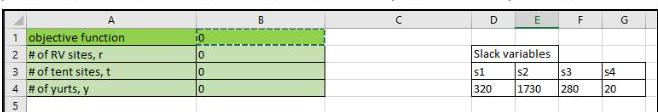
\includegraphics[scale = 0.5]{2022_07_05_5945264bba2a5f6ba667g-37-1}

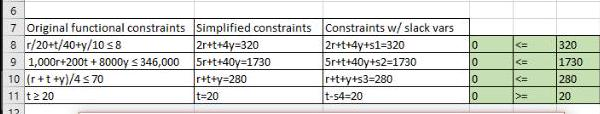
\includegraphics[scale = 0.5]{2022_07_05_5945264bba2a5f6ba667g-37-2}

$All Methods | GRG Nonlinear | Evolutionery |$

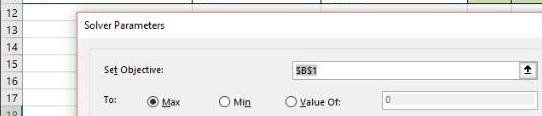
\includegraphics[scale = 0.5]{2022_07_05_5945264bba2a5f6ba667g-37(3)}

Constrainterecisioni. $\quad 0.000001 .$

- Automatic scaling

Whe Automatic scoling

Whow lteration results

Solving with integer Constraints

Solving with integer constraints

\begin{tabular}{l|l|l|}
18 & By Changing Variable Cells: & \$ \\
\hline
19 & SBS2:SBS4 &  \\
20 & Subject to the Constraints: & SDS11 = SFs11 \\
\hline
21 &  &  \\
\hline
\end{tabular}

$\square$ Ignoce integer constraints

By Changing Variable Cells:

$\mathrm{~ - ~ T ~ 2 ~}$

1

(2. $\quad$ Solving Limits

4

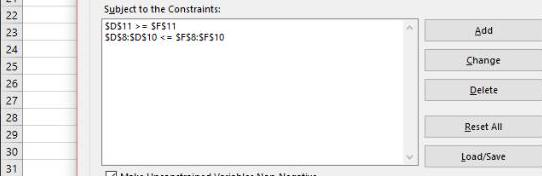
\includegraphics[scale = 0.5]{2022_07_05_5945264bba2a5f6ba667g-37(4)}

Subbject to the Constraints:

Max Iime |Seconds|:

Iterations:

Evolutionary and Integer Constraints:

Evolutionary and inteE

Lox subprobiems:

Mox Ecosible Solutions:

Options


\includegraphics[scale = 0.5]{2022_07_05_5945264bba2a5f6ba667g-37(5)}

\begin{itemize}
  \item 
\end{itemize}
$\square$ Make Unconstrained Variables Non-Negative

Select a Solving\\
Method:

ORtions

Solving Method

Solving Method Select the GRG Nonlinear engine for Solver Problems that are smooth nonlinear. Select the\\
Simplex engine for linear Solver Problems, and select the Evolutionary engine for Solver problems that are non-smooth.

Help

Solve

Close


\section{A Remark on BIP and Integer Programming}
In the previous examples, our solutions came out to be integers, even though we did not put that restriction in place. In the case that the solution to the LP problem is an integer, it is also so optimal solution to the Integer IP problem. However, usually the IP problem or BIP problem (binary integer program) are much harder to solve than the LP problem. Let's discuss why this is.

At first, it seems that IP and BIP problems should be easier to solve, after all, there is only a finite number of possible integer valued points in a bounded feasible region. An enumeration algorithm should work, just try all finite solution and pick the best. Assume we have a problem with $n$ variables. In the case of the BIP that means there are $2^{n}$ possible solutions to check. In the case of an IP problem, even if the variables are bound between say 0 and 10 , that is $11^{n}$ solution. The growth in complexity is exponential. While that may work for our class problems, actual OR problems typically have hundreds of thousands of variables.

So why don't we just solve the problem without the integer restriction (called the LP relaxation of the IP problem) and then round the result to the nearest integer? Have a look at the graphs below. On the left you see the feasible region, objective function, and solution $(4.2,3.8)$ for the relaxed problem. The direction of increase of the objective function is to the top left. Rounding either or both of the $x$ and $y$ coordinate of the solution up or down will result in a point outside the feasible region. On the right, you see all the feasible points. The solution to the IP problem is at $(0,3)$, not even close to the LP solution\\

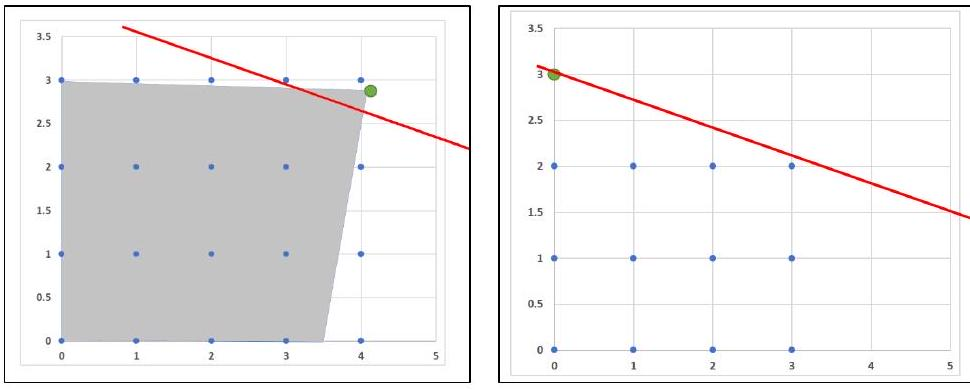
\includegraphics[max width=\textwidth]{2022_07_05_5945264bba2a5f6ba667g-38}

We will not address any of the solution strategies for IP and BIP problems. For this class, it suffices that Excel offers BIP and Integer constraint options.

\section{A Final Comment}
We completely ignore that LP requirement of divisibility, i.e. the fact that the decision variables could conceivably be fractions. In our current case study, fractional answers make no sense, one cannot build $.38$ of a yurt for example. Fortunately, this problem was carefully set up to ensure the solution came out as an integer. In real life, that won't be the case. Excel has the option to add an integer constraint to your decision variables.

There are a lot of methods to work around the strict LP requirements, for example the linearity requirement. If we have time, we will address some of them at the end of class. Meanwhile, if your group projects run into some issues with the LP requirements, please see me.

Now a developer comes and offers you $\$ 1,1$ million/acre. What do you do?

\section{NATIONAL PARK - NETWORKS AND ASSIGNMENT}
In this chapter, we will examine three types of problems:

\begin{enumerate}
  \item In allocation problems, a limited resource "supply" is allocated to various entities "demand". We will see what happens if demand exceeds supply and vice versa.

  \item Assignment problems assign exactly one of $n$ task to each of exactly $n$ workers

  \item Network problems look at a variety of issues arising in a network of nodes and arcs, from spanning trees to traversal problems.

\end{enumerate}
\section{Learning Goals}
\begin{itemize}
  \item Allocation problems

  \item Assignment problems

  \item Shortest path problem

  \item Flow problems

  \item Maximum flow

  \item Maximum flow - minimum cost

  \item Traveling salesman problem

  \item Using Excel to solve the above

\end{itemize}
\section{Case Study Description}
A very popular National Park is facing a number of challenges and has hired your company to propose solutions to the following:

\begin{enumerate}
  \item Due to budget cuts, much of the work in the park such as interpretive services and trail maintenance is done by volunteers. What is the most efficient way to assign them to the various tasks and locations? Also, you need to make sure each location has one full-time ranger on site.

  \item Traffic has gotten so bad that the park is considering banning personal vehicles on some roads and using shuttle busses instead. What should the bus routes be? How many busses are needed? Is a shuttle service even feasible?

  \item During winter, some of the park roads will be closed. However, enough roads need to be plowed to allow access to all ranger stations. Which roads should be plowed?

  \item A delivery truck needs to visit each of the parks location. What is the best route to take?

  \item All roads need to be patrolled daily. What is the best route for the ranger to take?

\end{enumerate}
Following is a simplified park map showing roads and attractions. As needed, you will also be provided with information regarding length, driving time, and shuttle capacity for each road segment.

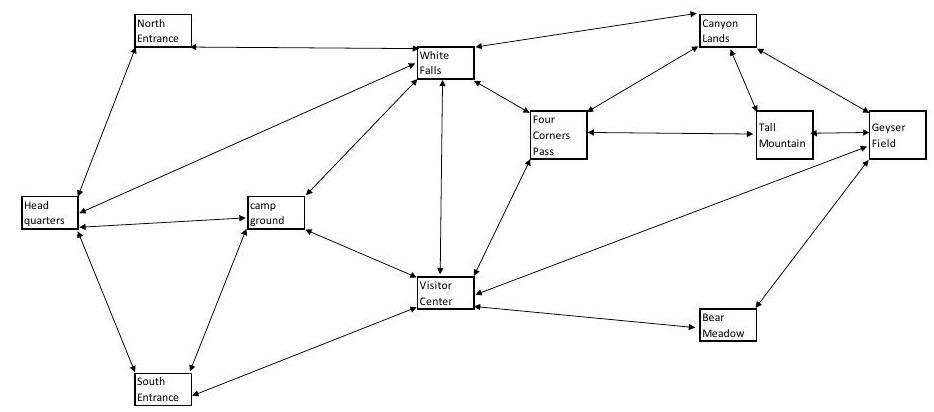
\includegraphics[max width=\textwidth]{2022_07_05_5945264bba2a5f6ba667g-41}

\section{References}
Budget cuts and overcrowding are very real issues for our National Parks. For more information on both, see:

\href{https://www.npca.org/articles/1500-budget-proposal-threatens-national-}{https://www.npca.org/articles/1500-budget-proposal-threatens-national-}

parks\#sm.0000ks3wtu35mdezurz1liyktck1t

\href{http://www.ournationalparks.us/park_issues/busy_parks_seek_approaches_to}{http://www.ournationalparks.us/park\_issues/busy\_parks\_seek\_approaches\_to} manag

e crowds cars/

\href{https://wWW.nps.gov/zion/planyourvisit/traffic.htm}{https://wWW.nps.gov/zion/planyourvisit/traffic.htm}

\href{http://www.triplepundit.com/2016/03/national-parks-face-crowding-degradation/}{http://www.triplepundit.com/2016/03/national-parks-face-crowding-degradation/}

\href{http://wwW.hcn.org/articles/arches-crowds-tourism-national-parks-utah}{http://wwW.hcn.org/articles/arches-crowds-tourism-national-parks-utah}

\href{https://www.nps.gov/yell/planyourvisit/visitationstats.htm}{https://www.nps.gov/yell/planyourvisit/visitationstats.htm}

\section{Part 1: Work Force - Resource Allocation}
Let's assume volunteers are available at the entrances to the park, HQ, NE, and SE. From there, you will have to transport them to the different locations and tasks. There is trail construction going on at VC and GF, so a lot of volunteers are needed there. GF is a very popular tourist destination, so lots of help is needed there as well. The cost/volunteer hour depends on a number of factors, such as distance to park entrance, nature of work, insurances required, etc. This table shows a summary of cost, supply, and demand.

We will denote each location by its initials, for example NE for North entrance, CL for Canyon lands etc. Four corners pass does not need any staffing, so we omit it.

This is an example of an allocation problem. A resource (volunteer hours, water rights, money, fish catch) is allocated to different areas (park location, cities, departments, canneries). In the ideal case, supply matches demand exactly. Let's start by assuming this is happening here:

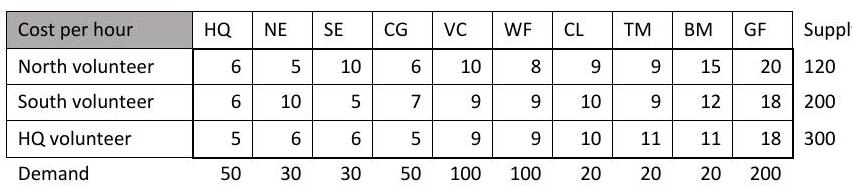
\includegraphics[max width=\textwidth]{2022_07_05_5945264bba2a5f6ba667g-42}

Note how the supply column and demand row add up to the same value, 620 . Your objective is to minimize cost while meeting demand. Note that in this ideal case supply = demand. This problem can be set up as a linear programming problem and solved with the simplex method. You should check that the assumptions for a LP problem hold.

To solve this problem with Excel, we set up a second table containing the decision variables, i.e. how many hours from which source are being allocated to which area. Initially, we set them all to zero. The highlighted cells contain formulas. We can now use the Excel solver.

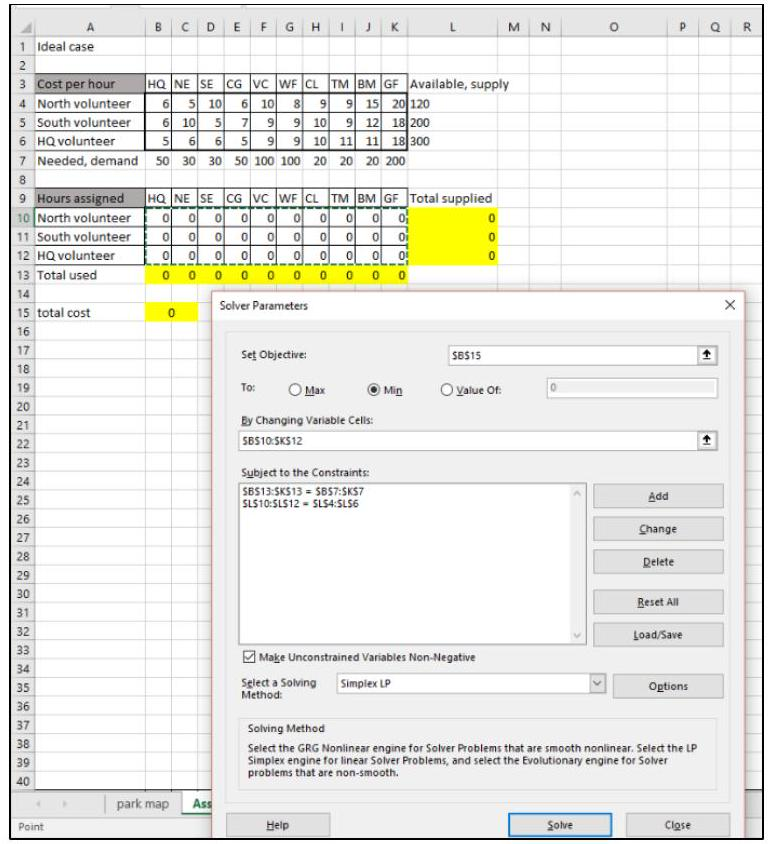
\includegraphics[max width=\textwidth]{2022_07_05_5945264bba2a5f6ba667g-42(1)}

The solver returns the solution, which the park can then implement, and the total weekly cost of $\$ 6710 .$

\begin{tabular}{|l|r|r|r|r|r|r|r|r|r|r|l|}
\hline
Hours assigned & HQ & NE & SE & CG & VC & WF & CL & TM & BM & GF & Total supplied \\
\hline
North volunteer & 0 & 0 & 0 & 0 & 0 & 100 & 20 & 0 & 0 & 0 & 120 \\
\hline
South volunteer & 0 & 0 & 30 & 0 & 0 & 0 & 0 & 20 & 0 & 150 & 200 \\
\hline
HQ volunteer & 50 & 30 & 0 & 50 & 100 & 0 & 0 & 0 & 20 & 50 & 300 \\
\hline
Total used & 50 & 30 & 30 & 50 & 100 & 100 & 20 & 20 & 20 & 200 &  \\
\hline
total cost & 6710 & \multicolumn{10}{c}{} \\
\hline
\end{tabular}

We were lucky and got integer value solutions. However, in this case the divisibility requirement of LP problems is satisfied, we could allow fractional hours worked.

\section{Refinements}
Let's assume you have too many volunteers, i.e. supply > demand. We incorporate them by assigning those hours we don't need to the "excess" column and proceeding otherwise just like before:

\begin{tabular}{|l|l|}
\hline
total cost & 0 \\
\hline
\end{tabular}

The table below shows the solution. Not surprisingly, with more volunteers available the overall cost went down.

\begin{tabular}{|l|c|c|c|c|c|c|c|c|c|c|c|}
\hline
Hours assigned & HQ & NE & SE & CG & VC & WF & CL & TM & BM & GF & not used \\
\hline
North volunteer & 0 & 30 & 0 & 0 & 0 & 100 & 20 & 20 & 0 & 0 & 30 \\
\hline
South volunteer & 0 & 0 & 30 & 0 & 100 & 0 & 0 & 0 & 0 & 20 & 100 \\
\hline
HQ volunteer & 50 & 0 & 0 & 50 & 0 & 0 & 0 & 0 & 20 & 180 & 0 \\
\hline
\end{tabular}

total cost 6680

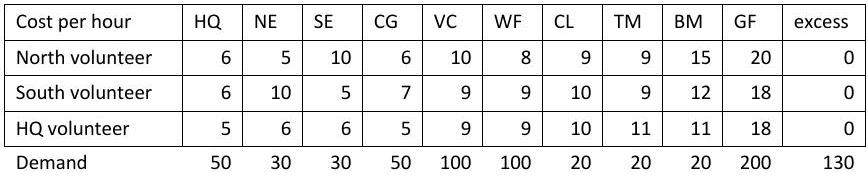
\includegraphics[max width=\textwidth]{2022_07_05_5945264bba2a5f6ba667g-43}

\begin{tabular}{|l|}
\hline
supply \\
\hline
200 \\
\hline
250 \\
\hline
300 \\
\hline
\end{tabular}

\begin{tabular}{|l|r|r|r|r|r|r|r|r|r|r|r|r|}
\hline
Hours assigned & \multicolumn{1}{|l|}{HQ} & \multicolumn{1}{l|}{NE} & \multicolumn{1}{l|}{SE} & \multicolumn{1}{l|}{CG} & VC & WF & CL & TM & BM & GF & excess \\
\hline
North volunteer & 0 & 0 & 0 & 0 & 0 & 0 & 0 & 0 & 0 & 0 & 0 \\
\hline
South volunteer & 0 & 0 & 0 & 0 & 0 & 0 & 0 & 0 & 0 & 0 & 0 \\
\hline
HQ volunteer & 0 & 0 & 0 & 0 & 0 & 0 & 0 & 0 & 0 & 0 & 0 \\
\hline
\end{tabular}

\begin{tabular}{|r|}
\hline
\multicolumn{1}{|l|}{Total supplied} \\
\hline
0 \\
\hline
0 \\
\hline
0 \\
\hline
\end{tabular}

If we have not enough volunteers, i.e. supply < demand, we adjust the table by introducing a row "missing volunteers". Let's also assume that the visitor center absolutely needs all its requested volunteers. We achieve that by making the cost for the "missing volunteers" $\$ 50000$, so high that that will not be an option.

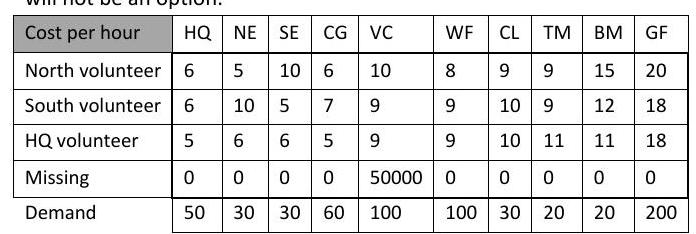
\includegraphics[max width=\textwidth]{2022_07_05_5945264bba2a5f6ba667g-44}

\begin{tabular}{|l|}
\hline
Supply \\
\hline
120 \\
\hline
200 \\
\hline
300 \\
\hline
20 \\
\hline
\end{tabular}

\begin{tabular}{|l|l|l|l|l|l|l|l|l|l|l|}
\hline
Hours assigned & HQ & NE & SE & CG & VC & WF & CL & TM & BM & GF \\
\hline
North volunteer & 0 & 0 & 0 & 0 & 0 & 90 & 30 & 0 & 0 & 0 \\
\hline
South volunteer & 0 & 0 & 30 & 0 & 100 & 10 & 0 & 20 & 0 & 40 \\
\hline
HQ volunteer & 50 & 30 & 0 & 60 & 0 & 0 & 0 & 0 & 20 & 140 \\
\hline
Missing & 0 & 0 & 0 & 0 & 0 & 0 & 0 & 0 & 0 & 20 \\
\hline
\multicolumn{1}{l}{Total used} & 50 & 30 & 30 & 60 & 100 & 100 & 30 & 20 & 20 & 200 \\
\hline
\end{tabular}

\begin{tabular}{|l|}
\hline
Total supplied \\
\hline
120 \\
\hline
200 \\
\hline
300 \\
\hline
20 \\
\hline
\end{tabular}

\begin{tabular}{|l|l|}
\hline
total cost & 6500 \\
\hline
\end{tabular}

Next consider the case where GF, not happy with losing 20 volunteers, specifies both the minimum supply and ideal supply. We again make it prohibitively expensive to not give them the minimum.

\begin{tabular}{|l|c|c|c|c|c|c|c|c|c|c|c|}
\hline
Cost per hour & HQ & NE & SE & CG & VC & WF & CL & TM & BM & GF min & GF+ \\
\hline
North volunteer & 6 & 5 & 10 & 6 & 10 & 8 & 9 & 9 & 15 & 20 & 20 \\
\hline
South volunteer & 6 & 10 & 5 & 7 & 9 & 9 & 10 & 9 & 12 & 18 & 18 \\
\hline
HQ volunteer & 5 & 6 & 6 & 5 & 9 & 9 & 10 & 11 & 11 & 18 & 18 \\
\hline
Missing & 0 & 0 & 0 & 0 & 50000 & 0 & 0 & 0 & 0 & 50000 & 0 \\
\hline
\multicolumn{1}{|c|}{Demand} & 50 & 30 & 30 & 60 & 100 & 100 & 30 & 20 & 20 & 190 & 10 \\
\hline
\end{tabular}

\begin{tabular}{|c|}
\hline
Supply \\
\hline
120 \\
\hline
200 \\
\hline
300 \\
\hline
20 \\
\hline
\end{tabular}

\begin{tabular}{|l|c|c|c|c|c|c|c|c|c|c|c|}
\hline
Hours assigned & $\mathrm{HQ}$ & $\mathrm{NE}$ & $\mathrm{SE}$ & $\mathrm{CG}$ & $\mathrm{VC}$ & $\mathrm{WF}$ & $\mathrm{CL}$ & $\mathrm{TM}$ & $\mathrm{BM}$ & $\mathrm{GF}$ min & $\mathrm{GF}+$ \\
\hline
North volunteer & 0 & 30 & 0 & 0 & 0 & 60 & 30 & 0 & 0 & 0 & 0 \\
\hline
South volunteer & 0 & 0 & 30 & 0 & 100 & 40 & 0 & 20 & 0 & 10 & 0 \\
\hline
HQ volunteer & 50 & 0 & 0 & 60 & 0 & 0 & 0 & 0 & 10 & 180 & 0 \\
\hline
Missing & 0 & 0 & 0 & 0 & 0 & 0 & 0 & 0 & 10 & 0 & 10 \\
\hline
Total used & 50 & 30 & 30 & 60 & 100 & 100 & 30 & 20 & 20 & 190 & 10 \\
\hline
\end{tabular}

\begin{tabular}{|c|}
\hline
Total supplied \\
\hline
120 \\
\hline
200 \\
\hline
300 \\
\hline
20 \\
\hline
\end{tabular}

\begin{tabular}{|l|l|}
\hline
total cost & 6570 \\
\hline
\end{tabular}

Finally, we need to assign exactly one ranger to each location. This is an example for an assignment problem, rather than having a resource that can be divided up, we have to make 1-1 assignments. We do this by setting both supply and demand totals to one, and using the solver constraints to set each decision variable to binary. If a certain ranger can't or won't work in a location, we just make the hourly cost too expensive for that particular assignment.

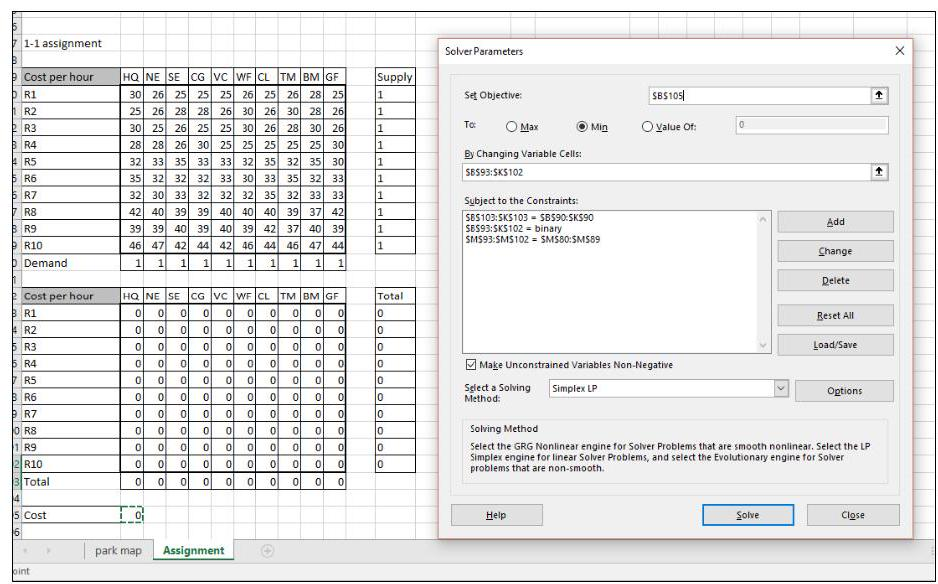
\includegraphics[max width=\textwidth]{2022_07_05_5945264bba2a5f6ba667g-45}

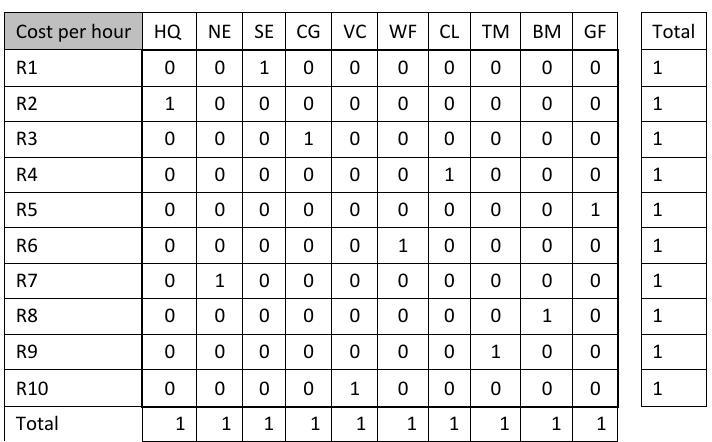
\includegraphics[max width=\textwidth]{2022_07_05_5945264bba2a5f6ba667g-45(1)}

\begin{tabular}{|l|l|}
\hline
Cost & 306 \\
\hline
\end{tabular}

If we had more rangers than needed, we would again add a placeholder column "not needed" and assign one of the rangers to it. If we had too few rangers, one of the locations would not get staffed, i.e. we d have an option "not staffed" as an additional row.

\section{Stating the Solution}
To minimize cost, rangers and volunteers should be assigned as follows (assuming exactly enough volunteers:

$\mathrm{R} 1 \rightarrow \mathrm{SE} \quad$ Assign the 120 NE volunteer hours as follows: 100 hours to WF, 20 hours to $C L$ $\mathrm{R} 2 \rightarrow \mathrm{HQ} \quad$ Assign the $200 \mathrm{SE}$ volunteer hours as follows: 30 hours to SE, 150 hours to GF R3 $\rightarrow$ CG Assign the 300 NE volunteer hours as follows: 50 hours to HQ, 30 hours to NE $\mathrm{R} 4 \rightarrow \mathrm{CL} \quad 50$ hours to CG, 100 hours to VC, 20 hours to $B M$, and 50 hours to GF

$\mathrm{R} 5 \rightarrow \mathrm{GF}$

$\mathrm{R} 6 \rightarrow \mathrm{WF}$

$\mathrm{R} 7 \rightarrow \mathrm{NE}$

$\mathrm{R} 8 \rightarrow \mathrm{BM}$

$\mathrm{R} 9 \rightarrow \mathrm{TM}$

$\mathrm{R} 10 \rightarrow \mathrm{VC}$

The total cost is $\$ 6,710 /$ hour for the volunteers and $\$ 306 /$ hour for the rangers.

Note that a similar set-up could be used to instead focus on worker preferences for assignments, their suitability for a task by ranking them, the driving distance to locations, or including urgency of assignments.

\section{Part 2: Shuttle service - Shortest Path and Maximum Flow}
We will examine two questions:

\begin{enumerate}
  \item What is the shortest route in terms of time from HQ to GF and

  \item Given the limited capacity of the narrow roads in the park, what is the maximum number of shuttle busses we can get from HQ to GF per hour? How much is it going to cost us? And how many visitors can we transport per hour?

\end{enumerate}
We will refer to the table on the next page listing distance, drive time, and capacity for each road segment in the park. Assume that driving time is the same in either direction, and that capacity is as well (i.e. we can run the full capacity in each direction). Instead of minimizing time, one could choose to maximize profit, maximize popularity, or minimize miles driven or incorporate constraints such as parking available at different locations or one-way roads.

\section{$\underline{\text { Shortest Path }}$}
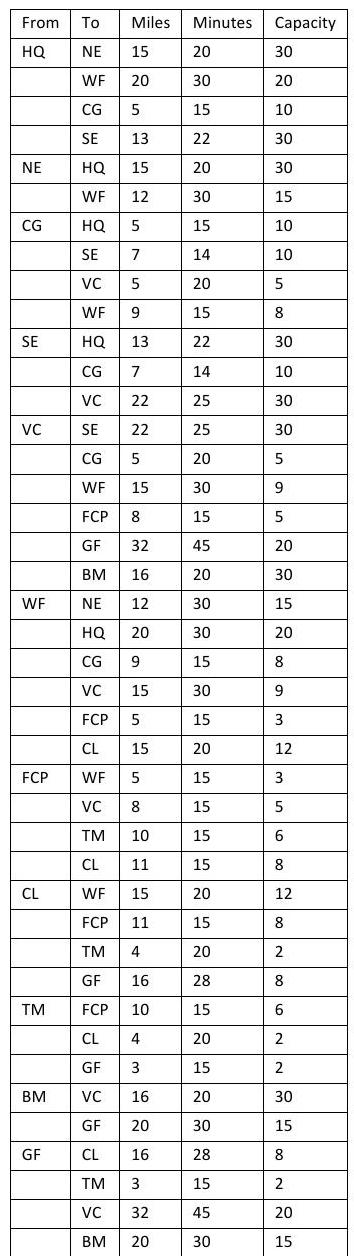
\includegraphics[max width=\textwidth]{2022_07_05_5945264bba2a5f6ba667g-47}

To find the shortest path from HQ to GF, we can start by deleting all the roads that are not needed. For example, if we start at $H Q$, we will not go back from NE to $H Q$.

Similarly, once we reach GF, we are done and do not need to leave again. This step is not strictly necessary to solve our small problem, but it is good form.

We will adopt terminology you may be familiar with from Discrete Structure. What we have here is a network problem. A network consists of nodes or vertices, the locations, and arcs, the roads. $A$ (directed) path from $A$ to $B$ is a sequence of connecting arcs where the direction is from A to $B$. The out-degree, $\mathbf{d e g}^{+}$of a node is the number of arcs originating at that node (leaving). The in-degree, deg $^{-}$, of a node is the number of arcs terminating at that node (entering). The net flow is $\mathrm{deg}^{+}$- deg. For our first question, we are looking for a shortest path from HQ to GF.

Because HQ is our start point, we want it to have a net flow of 1 . Our end point, GF, needs to have a net flow of $-1$, while all other nodes are either intermediate nodes or not used at all, so they all have zero net flow. You should convince yourself that this set-up guarantees a connected path from HQ to GF.

This problem can again be framed as a Linear Programming problem. We have a linear objective function to minimize, namely the sum of the times needed for all chosen paths. The decision variables, one for each path, have just two values. We set them $=1$ if the path is chosen, and $=0$ otherwise.

To compute net flow, we use the Sumlf function. The Sumlf function checks range\_1 for any value that meets the criteria, and if it finds them adds up the corresponding entries in the sum\_range.

Syntax: =Sumlf(range\_1, criteria, sum\_range) For details on how to set up the work sheet, refer to the screenshot below. There are two important things: First of all, the decision variables need to be constraint to be binary. That way, we avoid partial roads, which make no sense. Second, it is important to hold the ranges in the "Sumlf" statement fixed (use F4 key or $\$ \$$ signs)

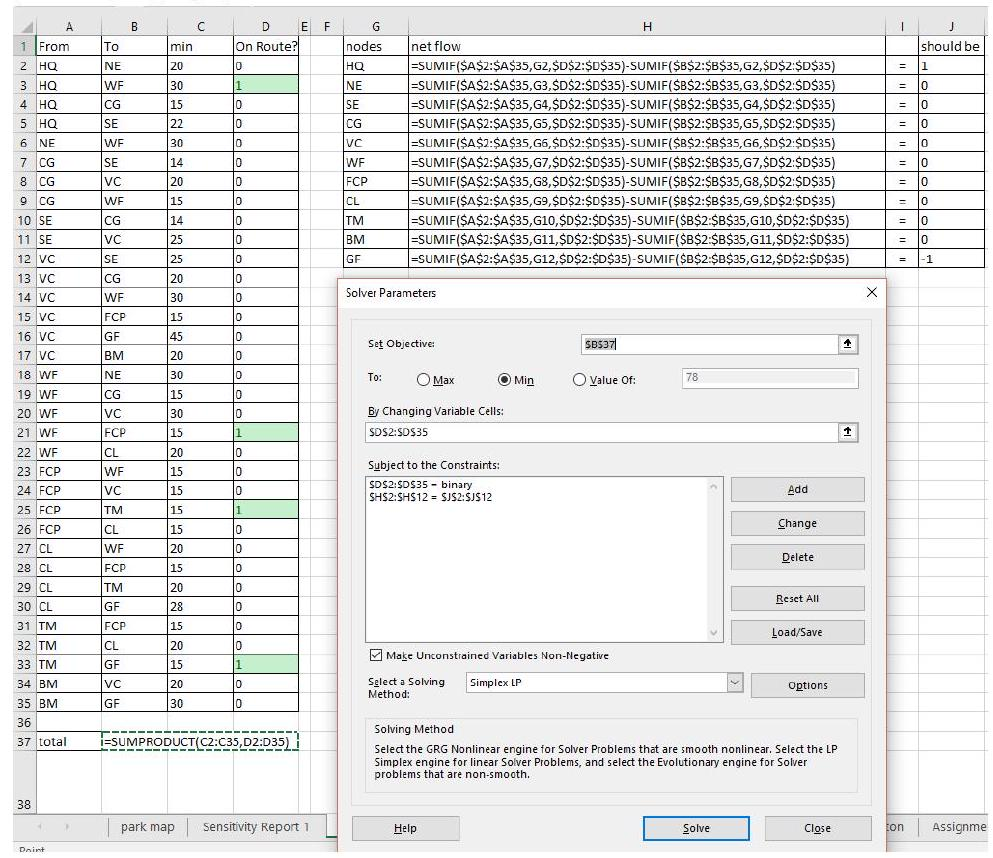
\includegraphics[max width=\textwidth]{2022_07_05_5945264bba2a5f6ba667g-48}

\section{Stating the Solution}
The solution turns out $\mathrm{HQ} \rightarrow \mathrm{WF} \rightarrow \mathrm{FCP} \rightarrow \mathrm{TM} \rightarrow \mathrm{GF}$ for a total of 75 minutes driving time. This is the shortest path (in terms of time) available. As far as the capacity is concerned, we need to use the minimum capacity for any of the four legs, which is 2 for TM to GF.

\section{Maximum Flow}
Two shuttles are not much, we will probably need more. How many shuttle busses total could we get from HQ to GF? And how can we do that with minimum total time? This question really asks us to solve a problem with two objective functions: Maximize flow while minimizing total time. To answer that question, we look at our park map, this time annotated with the capacities.

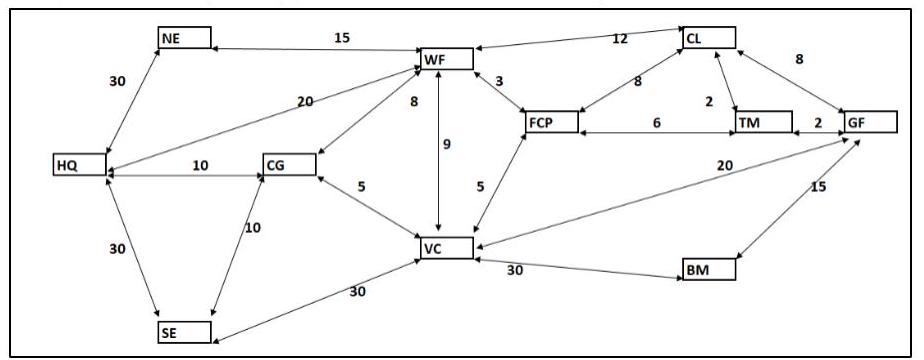
\includegraphics[max width=\textwidth]{2022_07_05_5945264bba2a5f6ba667g-49}

We already run 2 shuttles on $\mathrm{HQ} \rightarrow \mathrm{WF} \rightarrow \mathrm{FCP} \rightarrow \mathrm{TM} \rightarrow \mathrm{GF}$, so we change the numbers to reflect capacities still available. In effect, the road from TM to GF is no longer available. We eliminate that option from our list. (line 33).

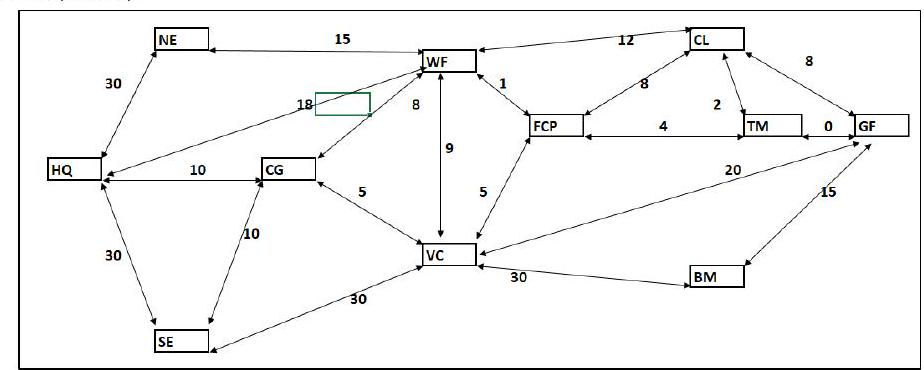
\includegraphics[max width=\textwidth]{2022_07_05_5945264bba2a5f6ba667g-49(1)}

Running the shortest path problem again (with one road less) gives us the path $\mathrm{HQ} \rightarrow \mathrm{WF} \rightarrow \mathrm{CL} \rightarrow \mathrm{F} \rightarrow \mathrm{GF}$, with 78 minutes. This route will accommodate 8 additional shuttles. We again adjust our map and table to reflect that yet another route is maxed out.

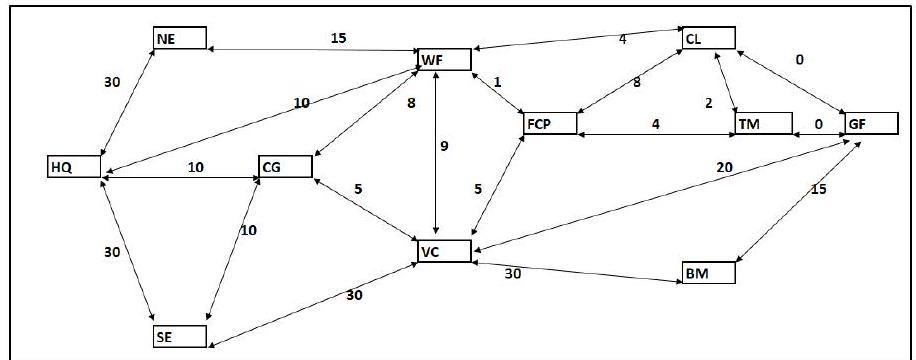
\includegraphics[max width=\textwidth]{2022_07_05_5945264bba2a5f6ba667g-49(2)}

We continue alternating the shortest path problem with adjusting route list and map, and arrive at the solution:

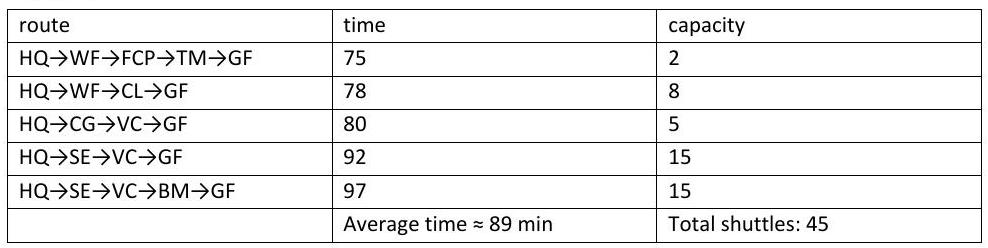
\includegraphics[max width=\textwidth]{2022_07_05_5945264bba2a5f6ba667g-50}

This is an example of a greedy algorithm. In each iteration, we pick what is best without considering the impact on future iterations. A greedy algorithm may, depending on the problem, have the effect that each iteration gives the optimal result given the previous iterations, but not necessarily the best result overall.

Following is a different, two-step approach. First, we solve the maximum flow problem without cost concerns. We use the max capacity as one of our constraints and allow the decision variables to be integers. The net flow is restricted only for the transitional nodes.

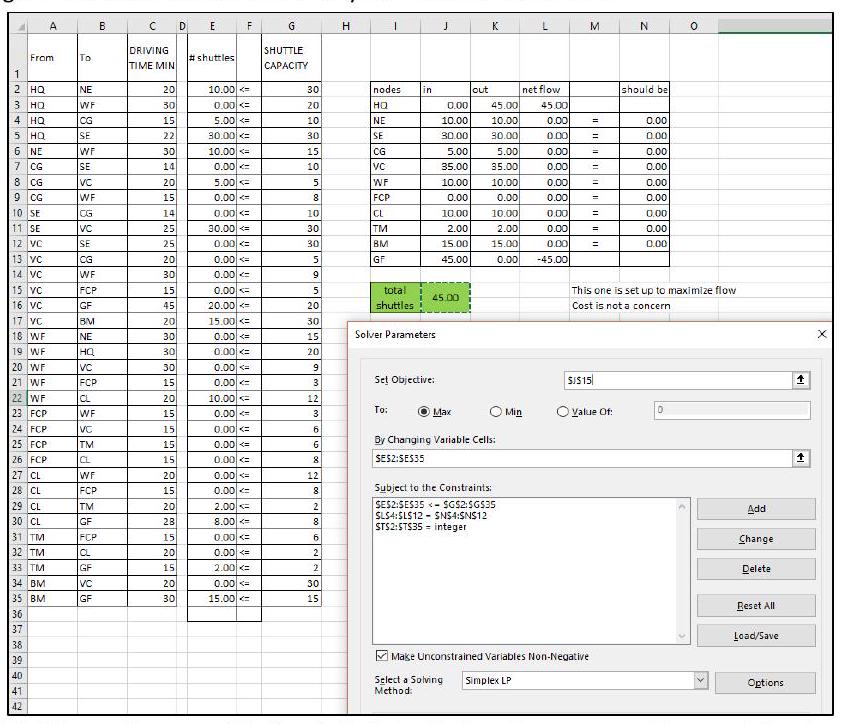
\includegraphics[max width=\textwidth]{2022_07_05_5945264bba2a5f6ba667g-50(1)}

We find that the maximum possible flow is 45 , just as before. Next, we can address cost (time).

\section{Maximum Flow - Minimum Cost}
To solve the maximum flow problem with cost constraints we use the result from the last section and modify the minimum cost problem. We set the netflow for our start point, HQ, to the maximum capacity and the netflow of our end point, GF, to the negative maximum capacity. Of course, we also change the objective function.

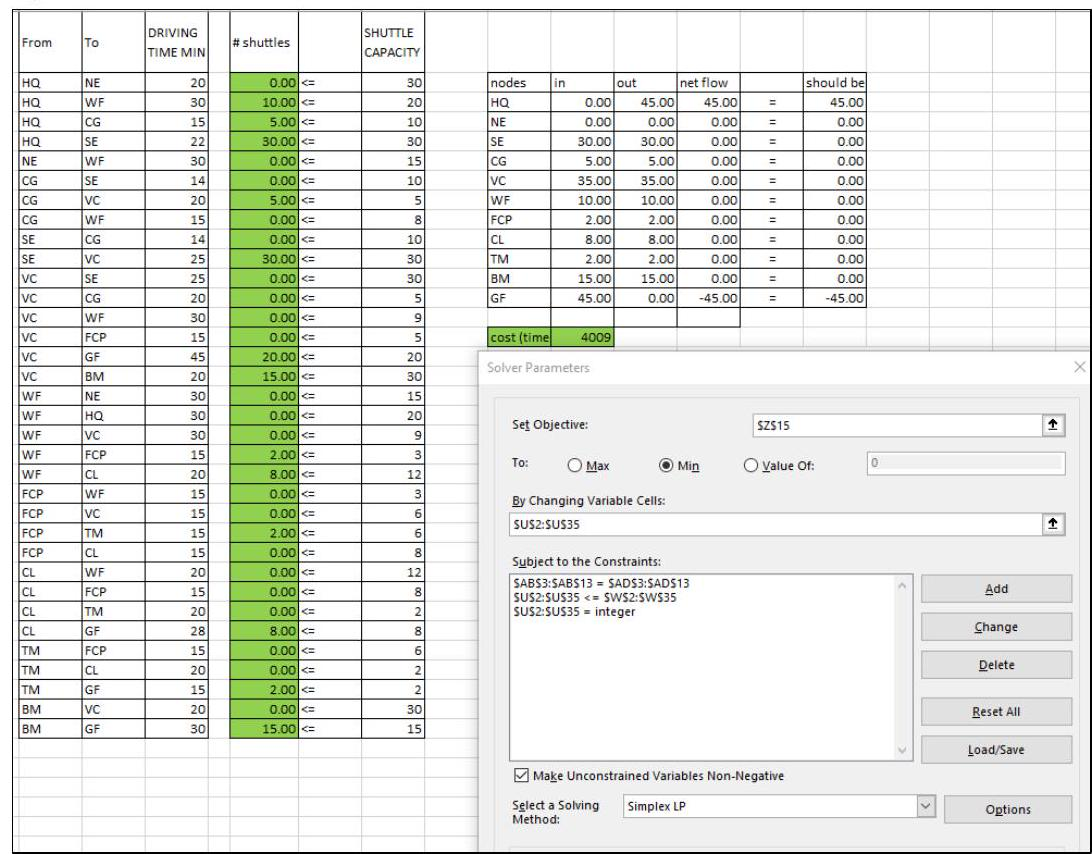
\includegraphics[max width=\textwidth]{2022_07_05_5945264bba2a5f6ba667g-51}

The average time needed is the same as before, $\approx 90$ minutes per shuttle. Note that you could use this last set-up to find the lowest average time for any number of shuttles, as long as the total stays at or below capacity.

While the total number of shuttles and the time needed is the same for both approaches, the routes taken are different. This is common for maximum flow problems. In fact, if you choose to solve a maximum flow problem by hand, it does not matter which route you start with.

\section{Stating the Solution}
If we use 50 passenger busses, we can transport 2250 passengers per hour using the maximum possible 45 shuttles per hour leaving HQ. Given that the roundtrip takes and average 90 minutes, and allowing 90 minutes at GF for sightseeing, this probably means we should start leaving $\mathrm{HQ}$ at 8 am and have the last shuttle leave no later than 4pm. This means we need 135 busses and can transport 18,000 passengers per day. This may not be enough (given that, for example, Yellowstone sees $900,000+$ visitors in July). We may have to consider bigger busses, wider roads, or restricting visitor numbers.

\section{Part 3: Plowing - Minimum Spanning Tree}
This problem is an example of a minimum spanning tree problem. A minimum spanning tree is a subset of a connected, weighted, undirected graph that connects all the nodes together in such a way that the total arc weight (cost) is minimized. There can be no cycles or loops, otherwise the tree would not be minimal.

Our plowing contractor charges by the mile, so we are trying to minimize distance, not driving time. Each road needs two passes, one in each direction. Here again a greedy algorithm works. Start with a graph showing all the locations (nodes), roads (arcs), and distances (weights). Build the tree by including the shortest roads first, but only if they do not create any loops. Add the next shortest roads, again watching out for loops. Continue until you have a connected tree.

We will add roads $\mathrm{TM} \rightarrow \mathrm{GF}(3), \mathrm{CL} \rightarrow \mathrm{TM}(4), \mathrm{WF} \rightarrow \mathrm{CL}(5), \mathrm{HQ} \rightarrow \mathrm{CG}(5), \mathrm{CG} \rightarrow \mathrm{VC}(5)$ successively.

\includegraphics[max width=\textwidth]{2022_07_05_5945264bba2a5f6ba667g-52}

Next are SE $\rightarrow$ CG (7) and VC $\rightarrow$ FCP $(8)$, but not CG $\rightarrow$ WF $(9)$ which would create a loop. We can add $\mathrm{TM} \rightarrow \mathrm{FCP}(10)$, but not $\mathrm{FCP} \rightarrow \mathrm{CL}(11)$

\includegraphics[max width=\textwidth]{2022_07_05_5945264bba2a5f6ba667g-53}

Finally, we add WF $\rightarrow$ NE $(12)$ and VC $\rightarrow \mathrm{BM}(16)$, for a total of 75 miles of road or 150 miles of plowing.

\includegraphics[max width=\textwidth]{2022_07_05_5945264bba2a5f6ba667g-53(1)}

This also tells us which roads can be closed in winter. Because we found a spanning tree, the contractor can start and end at any location or entrance.

\section{Stating the Solution}
To minimize cost, the following roads should be plowed:

$\mathrm{TM} \rightarrow \mathrm{GF}, \mathrm{CL} \rightarrow \mathrm{TM}, \mathrm{WF} \rightarrow \mathrm{CL}, \mathrm{HQ} \rightarrow \mathrm{CG}, \mathrm{CG} \rightarrow \mathrm{VC}, \mathrm{WF} \rightarrow \mathrm{NE}, \mathrm{SE} \rightarrow \mathrm{CG}, \mathrm{VC} \rightarrow \mathrm{FCP}, \mathrm{TM} \rightarrow \mathrm{FCP}$, and $V C \rightarrow \mathrm{BM}$, for a total of 150 miles of plowing. Contractors located at any of the three park entrances can be used with no difference in mileage, so the cheapest option should be used

\section{Part 4: Deliveries - Traveling Salesman Problem}
Assume you need to deliver supplies to each of the 11 locations in the park, starting and ending at HQ. You want to visit each location exactly once. In graph theory, a path that visits each vertex in a graph exactly once and ends and starts at the same vertex is called a Hamiltonian circuit. The problem of finding the minimum cost such path is called the Traveling Salesman Problem (TSP), probably the most famous problem in OR. This is a notoriously difficult problem to solve efficiently.

There are 11 locations to visit in a circuit. One could attempt to list all possible paths of length 11 , pick out the potential solutions (those through all 11 locations), compute the length and pick the best. The problem with this brute force approach is that there are so many possibilities. In the worst-case scenario, i.e. a complete graph with 11 vertices (complete means that each vertex is connected to every other vertex), there are $\frac{(n-1) !}{2}=\frac{10 !}{2}=1,814,400$ possible paths to check. While we do have only 21 edges instead of the 55 of a complete graph, it is still not feasible to find and check all potential paths.

We will use an approach called a heuristic, which is short for heuristic technique. A heuristic is an approach that uses a practical, often intuitive approach to problem solving. It is not guaranteed to yield the optimal result, but instead one that is "good enough" (hopefully),

\section{Nearest neighbor approach}
The nearest neighbor approach is fast, simple, and often yields a good short path. However, there are instances where it doesn't work at all or even yields the worst path. The idea is to start at an arbitrary vertex, chose the edge to the nearest unconnected vertex, and continue until the circuit is complete. This approach works well if the graph is complete or nearly so. In our case, starting at HQ, we end up "stuck", there is no path from BM back to NE:

\includegraphics[max width=\textwidth]{2022_07_05_5945264bba2a5f6ba667g-54}

You may have noticed that we had choices at FCP, however, each of them will lead to the same problem. There just aren't enough edges. One way around this is to use a modified nearest neighbor approach. We recognize that there are two nodes, NE and BM, where we do not have a choice how to reach them. We can therefor treat those segments (shown below) as a unit and try the nearest neighbor approach again.

\includegraphics[max width=\textwidth]{2022_07_05_5945264bba2a5f6ba667g-55}

Starting at HQ, this time we get a solution. The total length of this circuit is $209 .$

\includegraphics[max width=\textwidth]{2022_07_05_5945264bba2a5f6ba667g-55(1)}

\section{Sub-tour Reversal}
Next, we examine a technique called sub-tour reversal. We start with any possible directed circuit:

\includegraphics[max width=\textwidth]{2022_07_05_5945264bba2a5f6ba667g-55(2)}

This circuit is not - and doesn't have to be - perfect, it just serves as a starting point. The idea is to look at sub-tours, starting with one-segment ones, then two-segments, etc. We will look at each of those sub-tours and check if the total cost can be improved if we reverse direction. If we reverse direction, it will also affect the two path segments directly adjacent. We again start at HQ.

\includegraphics[max width=\textwidth]{2022_07_05_5945264bba2a5f6ba667g-56}

Of all three possible 1-segment subtour reversals, reversing $S E \rightarrow C G$ to $C G \rightarrow S E$ gives the best result, so we will implement that. Next, we check all two-segment sub-tours, then all three-segment sub-tours and so on (it turns out none of those are reversible). Our final circuit looks like this:

\includegraphics[max width=\textwidth]{2022_07_05_5945264bba2a5f6ba667g-57}

\section{TSP using Excel}
To use Excel to solve the TSP problem, we first have to set up the distance matrix. It shows the distance in minutes between each pair of nodes. As we have done earlier, we set this value to a large number when no such path exists to make sure that option is never chosen. Note that the matrix is symmetrical, this is because all our roads can be driven in either direction. If we had one-way roads the matrix would no longer be symmetrical.

This is no longer a linear programming problem. For example, we assign the different nodes arbitrary numbers, so the contribution of the decision variables to the value of the objective function is no longer proportional to their value. Excel offers two other solver options: A generalized reduced gradient algorithm and an evolutionary algorithm. The details of these algorithms are a bit beyond this class, though I am happy to talk to you outside the class room if you are interested. Basically, the GRG method finds the direction of steepest increase or decrease to move towards the maximum/minimum. It works well if the objective functions and feasible region are smooth-ish (think parabolas, cones, etc.). The evolutionary algorithm does not have any smoothness requirements. It uses a random start point and then evolves the next generation of solution points from that start point (a little like the path-reversal, but with a strong random element). It does not use gradient information, so you cannot be sure you reached the best solution. The evolutionary solver will keep searching for better solutions until it no longer makes sufficient progress or runs out of time. We will use the Evolutionary Solver option.

We start with an arbitrary sequence 1-2-3-4-5-6-7-8-9-10-11-1. The INDEX function is used to look the associated time in the distance matrix.

Syntax: =INDEX(range where to look, what row to use, optional: what column to use) The objective function is simply the sum of the times. As our only constraint we use the "all different" option. The constraint "\$C\$22:\$C\$32 = AllDifferent" means that the 11 decision variables stored in $\$ C \$ 22: \$ C \$ 32$ must be integers in the range $1-11$, with each one different from all the others, i.e. we require permutations of $\{1,2,3,4,5,6,7,8,9,10,11\}$. Finally, you want to choose the option to set a time limit for your solver, 60 seconds should be sufficient.\\

\includegraphics[max width=\textwidth]{2022_07_05_5945264bba2a5f6ba667g-58}

E $\quad$ F

\includegraphics[max width=\textwidth]{2022_07_05_5945264bba2a5f6ba667g-58(1)}\\

\includegraphics[max width=\textwidth]{2022_07_05_5945264bba2a5f6ba667g-58(2)}

\includegraphics[max width=\textwidth]{2022_07_05_5945264bba2a5f6ba667g-58(3)}\\

\includegraphics[max width=\textwidth]{2022_07_05_5945264bba2a5f6ba667g-58(4)}

\includegraphics[max width=\textwidth]{2022_07_05_5945264bba2a5f6ba667g-58(5)}

The solver returns the solution below. The time requirement is the same as we found in our previous attempts.

\begin{tabular}{|c|c|l|}
\cline { 2 - 3 }
 & Circuit & Time \\
\hline
WF & 6 & 20 \\
\hline
CL & 8 & 15 \\
\hline
FCP & 7 & 15 \\
\hline
TM & 9 & 15 \\
\hline
GF & 10 & 30 \\
\hline
BM & 11 & 20 \\
\hline
VC & 5 & 15 \\
\hline
SE & 3 & 14 \\
\hline
CG & 4 & 15 \\
\hline
HQ & 1 & 20 \\
\hline
NE & 2 & 30 \\
\hline
WF & 6 &  \\
\hline
\end{tabular}

\section{Stating the Solution}
Starting at $\mathrm{HQ}$, the route traveled will take 209 minutes or 3 hours 29 minutes. An optimal route to take is $\mathrm{HQ} \rightarrow \mathrm{NE} \rightarrow \mathrm{WF} \rightarrow \mathrm{CL} \rightarrow \mathrm{FCP} \rightarrow \mathrm{TM} \rightarrow \mathrm{GF} \rightarrow \mathrm{BM} \rightarrow \mathrm{VC} \rightarrow \mathrm{SE} \rightarrow \mathrm{CG} \rightarrow \mathrm{HQ} .$ An alternate of same length is $\mathrm{HQ} \rightarrow \mathrm{NE} \rightarrow \mathrm{WF} \rightarrow \mathrm{FCP} \rightarrow \mathrm{CL} \rightarrow \mathrm{TM} \rightarrow \mathrm{GF} \rightarrow \mathrm{BM} \rightarrow \mathrm{VC} \rightarrow \mathrm{SE} \rightarrow \mathrm{CG} \rightarrow \mathrm{HQ}$, and of course both routes can be reversed.

\section{Part 5: Road Patrols - Traversing}
To ensure the safety of visitors, a ranger has to patrol the entire road system in the park daily, starting and ending at HQ while minimizing travel time. If possible, they should drive each road only once in either direction. In graph theory, a path that visits each arc in a graph exactly once and ends and starts at the same vertex is called a Eulerian circuit. You may recall from Discrete Mathematics that a Euler circuit exists if and only if the degree of each vertex is even, i.e. an even number of edges connect to each vertex. Unfortunately, that is not the case here, SE and TM both have degree $3 .$

\includegraphics[max width=\textwidth]{2022_07_05_5945264bba2a5f6ba667g-59}

We already know that it is not possible to traverse each road exactly once, so the question now becomes how many times each road needs to be traveled, and in which direction. We re-arrange our table to list both road directions next to each other. This makes it easier to write the constraints: "each segment needs to be traveled at least once in either direction".

\includegraphics[max width=\textwidth]{2022_07_05_5945264bba2a5f6ba667g-59(1)}

\section{Stating the Solution}
It will take a single ranger 514 minutes or 8 hours 34 minutes to patrol all the roads in the park. One possible optimal route is:

$\mathrm{HQ} \rightarrow \mathrm{NE} \rightarrow \mathrm{WF} \rightarrow \mathrm{HQ} \rightarrow \mathrm{CG} \rightarrow \mathrm{WF} \rightarrow \mathrm{FCP} \rightarrow \mathrm{VC} \rightarrow \mathrm{WF} \rightarrow \mathrm{CL} \rightarrow \mathrm{FCP} \rightarrow \mathrm{TM} \rightarrow \mathrm{GF} \rightarrow \mathrm{CL} \rightarrow \mathrm{TM} \rightarrow \mathrm{FCP} \rightarrow \mathrm{VC} \rightarrow \mathrm{GF} \rightarrow \mathrm{BM} \rightarrow \mathrm{VC}$

$\rightarrow \mathrm{CG} \rightarrow \mathrm{SE} \rightarrow \mathrm{VC} \rightarrow \mathrm{SE} \rightarrow \mathrm{HQ}$. This is just one of many options. The only rule is that either all roads have to be travelled in the direction and frequencies shown, or all directions have to be reversed.

\includegraphics[max width=\textwidth]{2022_07_05_5945264bba2a5f6ba667g-60}

The patrol as specified is not possible without overtime, especially not if anything needs attention.

Possible alternatives are:

\begin{itemize}
  \item Splitting the area between two or more patrols or two or more days

  \item Eliminating roads from the patrol

  \item Faster car?

\end{itemize}
Comment: Note that this is a Euler path if you eliminate the second traversals. Basically, we have a Euler path from SE to TM + the fastest way / shortest path linking the beginning and end of that Euler path. If you think of each arrow as an undirected arc, then all nodes have even degree and a Euler circuit exists. Basically, we figured out where edges need to be added to have the cheapest possible Euler path/circuit.

\section{GAS EXPLORATION - DECISION ANALYSIS}
\section{Learning Goals}
In this chapter, you will learn how to organize a situation with different possible courses of action and associated outcomes into a flowchart (decision tree). We will examine how to incorporate uncertainty, expected values, and conditional probabilities to determine optimal strategies. To quote (Hillier \& Lieberman, 2005): "Decision Analysis provides a framework and methodology for rational decision making when the outcomes are uncertain".

\section{Case Study Description}
Your company is interested in exploring fracking for gas in Pennsylvania. You just signed a six-year lease on a promising tract of land, and you now have to decide how to proceed. Here are the parameters:

\begin{itemize}
  \item 1000 -acre tract

  \item Annual lease is $\$ 5 /$ acre paid up front $+15 \%$ royalty

  \item One time signing bonus of $\$ 200 /$ acre

  \item $50-50$ chance of productive

  \item It'll cost \$6 million to drill a well, potential for three wells

  \item After deducting royalties, each well could bring profit of $\$ 15$ million over six years of productive life span

  \item Option to do seismic survey at \$4 million, but a survey is not $100 \%$ accurate. In fact, we will assume that a survey will detect gas - if there is any - with $85 \%$ probability, but might also return a positive result with $5 \%$ probability if there really is not enough gas to drill (false positive)

  \item A positive survey would bring the value of your lease to $\$ 10$ million, you could sell that lease

  \item A negative survey would drop the value of your lease to $\$ 0$

  \item If you sell without a survey, you are confident you could sell the lease for $\$ 300,000$.

\end{itemize}
\section{References}
For further reading on the economics of gas exploration, see the following websites: \href{http://extension.psu.edu/publications/ua448/view}{http://extension.psu.edu/publications/ua448/view} \href{http://marcelluscoalition.org/wp-content/uploads/2016/10/FINAL-Post-Production-}{http://marcelluscoalition.org/wp-content/uploads/2016/10/FINAL-Post-Production-}

Toolkit 100616.pdf \href{http://extension.psu.edu/natural-resources/natural-gas/news/2010/11/seismic-surveying}{http://extension.psu.edu/natural-resources/natural-gas/news/2010/11/seismic-surveying} \href{http://geology.com/royalty/production-decline.shtml}{http://geology.com/royalty/production-decline.shtml}

\section{Solution Approach}
As you can tell, there are lots of options to choose from. We will organize them in a decision tree. Note that there are some nodes that allow you to make a decision, and others where nature/fate/luck comes in. Read the tree left to right.

\includegraphics[max width=\textwidth]{2022_07_05_5945264bba2a5f6ba667g-62}

Next, we add the cost of each decision in million $\$$ and the total cost for each path taken. Negative numbers stand for costs/losses.

\includegraphics[max width=\textwidth]{2022_07_05_5945264bba2a5f6ba667g-62(1)}

You immediately see that the best-case scenario would be to not do a survey, drill and find gas but of course that depends on being lucky. This is where we use statistics to compute the probabilities of each scenario, and the expected values of each action. We are given the following:

$\begin{array}{ll}P(\text { gas })=0.5 & P(\text { no gas })=0.5 \\ P(\text { positive survey } \mid \text { gas })=0.85 & P(\text { positive survey } \mid \text { no gas })=0.05 \\ \text { These imply: } & \\ P(\text { negative survey } \mid \text { gas })=0.15 & P(\text { negative survey } \mid \text { no gas })=0.95\end{array}$

What we really need to know is the probability that a positive survey means that there really is gas, $P$ (gas | positive survey). This a case for Bayes Law. Bayes Law states:

For a given partition $B_{1}, B_{2}, B_{3}, \ldots$ and an event $A:$
$$
P\left(B_{1} \mid A\right)=\frac{P\left(A \mid B_{1}\right) \cdot P\left(B_{1}\right)}{P\left(A \mid B_{1}\right) \cdot P\left(B_{1}\right)+P\left(A \mid B_{2}\right) \cdot P\left(B_{2}\right)+P\left(A \mid B_{3}\right) \cdot P\left(B_{3}\right) \ldots}
$$
In our case:

$P($ gas $\mid$ positive survey $)=\frac{P(\text { positive survey } \mid \text { gas }) \cdot P(\text { gas })}{P(\text { positive survey } \mid \text { gas }) \cdot P(\text { gas })+P(\text { positive survey } \mid \text { no gas }) \cdot P(\text { gas })}=\frac{0.85 \cdot 0.5}{0.85 \cdot 0.5+0.05 \cdot 0.5}=\frac{17}{18}$ and therefore $P($ no gas $\mid$ positive survey $)=\frac{1}{18}$.

Similarly $P($ gas $\mid$ negative survey $)=\frac{3}{22}$ and $P($ no gas $\mid$ negative survey $)=\frac{19}{22}$.

So, if you have a positive survey and drill, you have a 17/18 chance of finding a lot of gas and making $\$ 22.77$ million, and a 1/18 chance of finding nothing and losing $\$ 22.23$ million. In other words, the conditional expectations are
$$
\mathrm{E}[\text { drill } \mid \text { positive survery }]=\frac{17}{18} \cdot 22.77-\frac{1}{18} \cdot 22.23=20.27
$$
and
$$
\mathrm{E}[\text { drill } \mid \text { negative survery }]=\frac{3}{22} \cdot 22.77-\frac{19}{22} \cdot 22.23=-16.094 \text {. }
$$
Of course, $E[$ sell $\mid$ positive survey $]=5.77$ and $E[$ sell $\mid$ negative survey $]=-4.23$.

In summary, if you drill after a positive survey, your expected return of $\$ 20.27$ million is better than what you would earn under the alternative (don't drill, sell), so you discard the selling option. We call this "pruning the tree". Similarly, if you have a negative survey, you should sell to minimize your expected loss.

If you don't pay for a survey and just drill, you have a 50-50 chance of finding gas and your expected return is $E[$ drill, no survey $]=0.5 \cdot 23.77-0.5 \cdot 18.23=1.108$, still better than what you can expect if you don't do a survey and just re-sell your lease. Here is the "pruned" decision tree with just the optimal decisions and expected values in [] identified so far:

\includegraphics[max width=\textwidth]{2022_07_05_5945264bba2a5f6ba667g-64}

So, should you pay for a survey in the first place? To answer that, we need to find a few more probabilities and expected values. We will have to use the Law of Total Probability and the definition of conditional probability. For a given partition $B_{1}, B_{2}, B_{3}, \ldots$ and an event $A:$
$$
P(A)=P\left(A \cap B_{1}\right)+P\left(A \cap B_{2}\right)+P\left(A \cap B_{3}\right) \ldots=P\left(A \mid B_{1}\right) \cdot P\left(B_{1}\right)+P\left(A \mid B_{2}\right) \cdot P\left(B_{2}\right)+P\left(A \mid B_{3}\right) \cdot P\left(B_{3}\right) \ldots
$$

\section{Therefore,}
$$
\begin{aligned}
\mathrm{P}(\text { positive survey }) &=P(\text { positive survey } \mid \text { gas }) \cdot P(\text { gas })+P(\text { positive survey } \mid \text { no gas }) \cdot P(\text { no gas }) \\
&=0.5 \cdot 0.85+0.5 \cdot 0.05=0.45 \\
P(\text { negative survey }) &=P(\text { negative survey } \mid \text { gas }) \cdot P(\text { gas })+P(\text { negative survey } \mid \text { no gas }) \cdot P(\text { no gas }) \\
&=0.5 \cdot 0.15+0.5 \cdot 0.95=0.55
\end{aligned}
$$
Assuming you follow the optimal strategies, your expected return if you choose to conduct a survey is $\mathrm{E}[$ survey $]=0.45 \cdot 20.27-0.55 \cdot 4.23=6.795$. This is much better than the best outcome for not conducting a survey, which was $1.108 .$

\includegraphics[max width=\textwidth]{2022_07_05_5945264bba2a5f6ba667g-65}

\section{Stating the Solution}
Under the given parameters, the optimal strategy is to buy the lease and conduct a survey. In the case of a positive survey, one should drill and can expect a profit of $\$ 20.27$ million. If the survey is negative, one should sell the lease to minimize the loss, $\$ 4,23$ million.

Worst case scenario under optimal strategy: Company drills and finds no gas, looses $\$ 22.23$ million Best case scenario under optimal strategy: Company drills and finds gas, profit of $\$ 22.77$ million

\section{ROCK PAPER SCISSORS - GAME THEORY}
\section{Learning Goals}
In this section, you will learn how to set up payoff tables, use and evaluate different game strategies, and use probabilities to find an optimal mixed strategy for zero sum games. You should also be able to tell if a game is fair.

\section{Case Study Description - Rock-Paper-Scissors}
On the "Big Bang Theory", the guys tried to improve the old game "rock-papers scissors". However, the new version still produces ties $20 \%$ of the time. After we study some of the intricacies of games, we (by that I mean you) will be able come up with a version that will give us a better chance at winning against Sheldon et al.

\section{References}
If you are interested in learning more about game theory, Steven Brams' book on Game Theory and politics (Brams, 2004) is a good source of often surprising applications. The updated 2004 edition addresses topics ranging from the classical "prisoners' dilemma" to voting strategies and studies of historic battle plans. A video of the relevant Big Band episode is here: (Big Bang Theory, 2008).

\section{Solution Approach}
It is common to summarize a game with a payoff table. The table shows strategies for both players ("We" and "They") and outcomes for one of the players (us). As you can see, no matter which strategy we choose, we have a $1 / 2$ chance of winning, tying the game, or losing. Overall, those same probabilities hold: $3 / 9$ chance of win, lose, draw.

\begin{tabular}{|r|l|r|r|r|}
\hline
 &  &  &  &  \\
\hline
 &  & Rock & Paper & Scissors \\
\hline
 & Rock & 0 & $-1$ & 1 \\
\hline
 & Paper & 1 & 0 & $-1$ \\
\hline
 & Scissors & $-1$ & 1 & 0 \\
\hline
\end{tabular}

Before we go further, let's list some assumptions and definitions:

We are assuming all players are rational

We are assuming both players play to win

In a zero-sum game, one player wins whatever the other player loses.

A fair game is a game that is not biased towards one of the players; if both players play optimally, they both have the same expected return of. Rock paper scissors is an example of a fair, zero-sum game. Adding the additional strategies "lizard" and "Spock" increases the size of the table and reduces the odds of a tie to $1 / 5$, but still doesn't substantially change the game.

\begin{tabular}{|l|r|r|r|r|r|}
\hline
 & \multicolumn{1}{|l|}{Rock} & \multicolumn{1}{l|}{Paper} & \multicolumn{1}{l|}{Scissors} & Lizard & \multicolumn{1}{l|}{Spock} \\
\hline
Rock & 0 & $-1$ & 1 & 1 & $-1$ \\
\hline
Paper & 1 & 0 & $-1$ & $-1$ & 1 \\
\hline
Scissors & $-1$ & 1 & 0 & 1 & $-1$ \\
\hline
Lizard & $-1$ & 1 & $-1$ & 0 & 1 \\
\hline
Spock & 1 & $-1$ & 1 & $-1$ & 0 \\
\hline
\end{tabular}

\section{Approach 1: Maximizing expected return}
One possible game plan is to choose the strategy that yields the greatest average return. In the table above, that doesn't help because, if both players randomly chose what to throw, i.e. if each strategy has the same $1 / 5$ probability of being chosen, then each strategy has an expected value of 0 . But in the video we watched in class, they complain that everyone always chooses "Spock". Adding probabilities changes the game:

\begin{tabular}{|l|l|l|l|l|l|}
\hline
probability & $0.05$ & $0.05$ & $0.1$ & $0.1$ & $0.7$ \\
\hline
 & Rock & Paper & Scissors & Lizard & Spock \\
\hline
Rock & 0 & $-1$ & 1 & 1 & $-1$ \\
\hline
Paper & 1 & 0 & $-1$ & $-1$ & 1 \\
\hline
Scissors & $-1$ & 1 & 0 & 1 & $-1$ \\
\hline
Lizard & $-1$ & 1 & $-1$ & 0 & 1 \\
\hline
Spock & 1 & $-1$ & 1 & $-1$ & 0 \\
\hline
\end{tabular}

We find that under these circumstances, we should play Lizard, because that has the highest expected return.

A possible refinement would be to assign value to each item. For example, rocks are cheap, so losing a rock could be equated with losing 1 point, paper 2 points, scissors 3 points, Lizard 4, and Spock $5 .$

Assuming equal probabilities, this results in the following pay-off table and expected returns:

\includegraphics[max width=\textwidth]{2022_07_05_5945264bba2a5f6ba667g-67}

We see that now "Rock" is the best strategy for both parties with an expected return of 0 for everyone. Of course, if They think we will play "Rock", They may change their strategy to "Paper" or "Spock", so we should change to "Lizard", which will cause Them to change to "Rock" or "Scissors", which makes us go to "Spock", etc. etc...

\section{Approach 2: Minimizing potential loss}
Another strategy, especially for risk adverse people, is to minimize potential loss. We again use the payoff table, but this time we find the maximum potential loss for each strategy, we perform a worstcase analysis:

\begin{tabular}{|l|r|r|r|r|r|}
\hline
 & \multicolumn{1}{|c|}{Rock} & Paper & Scissors & Lizard & Spock &  \\
\hline
Rock & 0 & $-1$ & 3 & 4 & $-1$ &  \\
\hline
Paper & 1 & 0 & $-2$ & $-2$ & 5 &  \\
\hline
Scissors & $-3$ & 2 & 0 & 4 & $-3$ &  \\
\hline
Lizard & $-4$ & 2 & $-4$ & 0 & 5 &  \\
\hline
Spock & 1 & $-5$ & 3 & $-5$ & 0 &  \\
\hline
max loss for Them &  & \multicolumn{5}{|l|}{max loss for Us} \\
\hline
\end{tabular}

Both players should use "rock" as their strategy, as it minimizes potential losses for both parties. Again, once the other team notices our strategy, they will change theirs, which will make us change ours, and so forth.

\section{Approach 3: Looking for a saddle point}
Let's assume we just assign letters to each strategy, and values to the outcomes as shown in the table below. The strategies that minimize potential loss are "C" for Us and "B" for Them. The outcome is the same for both players, 0 , so this is a fair game. Note that, unlike any of the two previous scenarios, no party benefits from unilaterally changing their strategy. If either party changes their strategy without the other changing as well, their outcome will get worse. On the other hand, having a game like this were the outcome can be reasoned out beforehand and both players are risk adverse is also somewhat boring.\\

\includegraphics[max width=\textwidth]{2022_07_05_5945264bba2a5f6ba667g-68}

\section{Approach 4: Looking for dominated strategies}
Sometimes one finds looking at the payoff table that one strategy is always better than another. For example, in the table below, strategy "C" is better for Them than either strategy A or $E$. We say "C dominates $D$ and $E^{\prime \prime}$

\begin{tabular}{r|r|r|r|r|r|}
 & \multicolumn{1}{c}{A} &  & $C$ & $D$ & $E$ \\
\cline { 2 - 6 }
A & $-1$ & 1 & $-1$ & 1 & $-1$ \\
\cline { 2 - 5 }
B & 2 & $-2$ & $-2$ & 0 & 2 \\
\cline { 2 - 5 }
C & $-1$ & $-4$ & $-3$ & 2 & $-2$ \\
\cline { 2 - 5 }
D & 2 & 1 & 1 & 2 & 1 \\
\cline { 2 - 6 }
E & 2 & 3 & $-3$ & 2 & $-2$ \\
\hline
\end{tabular}

If $C$ is always better, then there is no reason for Them to use strategies $A$ or $E$, we can eliminate them.

\begin{tabular}{r|r|r|r|r|r|}
\multicolumn{1}{r}{} & $A$ & $B$ & $C$ & $D$ & $E$ \\
\hline
A & $-1$ & 1 & $-1$ & 1 & $-1$ \\
\hline
B & 2 & $-2$ & $-2$ & 0 & 2 \\
\cline { 2 - 6 }
$C$ & $-1$ & $-4$ & $-3$ & 2 & $-2$ \\
\cline { 2 - 6 }
D & 2 & 1 & 1 & 2 & 1 \\
\cline { 2 - 6 }
E & 2 & 3 & $-3$ & 2 & $-2$ \\
\hline
\end{tabular}

Now we see that for Us, D dominates $A, B$, and $C$, so we can eliminate them as well.

\begin{tabular}{rr|r|r|r|r|}
 & \multicolumn{1}{c}{A} &  & $C$ & D & E \\
\cline { 2 - 6 }
A & $-1$ & 1 & $-1$ & 1 & $-1$ \\
\cline { 2 - 6 }
B & 2 & $-2$ & $-2$ & 0 & 2 \\
\hline
C & $-1$ & $-4$ & $-3$ & 2 & $-2$ \\
\cline { 2 - 6 }
D & 2 & 1 & 1 & 2 & 1 \\
\cline { 2 - 6 }
E & 2 & 3 & $-3$ & 2 & $-2$ \\
\cline { 2 - 6 }
\end{tabular}

Now, for Them, strategy $C$ dominates $D$ and $B$.

\begin{tabular}{r|r|r|r|r|r|}
\hline
 & $A$ & $B$ & $C$ & $D$ & $E$ \\
\hline
A & $-1$ & 1 & $-1$ & 1 & $-1$ \\
\cline { 2 - 6 }
B & 2 & $-2$ & $-2$ & 0 & 2 \\
\cline { 2 - 6 }
$C$ & $-1$ & $-4$ & $-3$ & 2 & $-2$ \\
\cline { 2 - 6 }
D & 2 & 1 & 1 & 2 & 1 \\
\cline { 2 - 6 }
E & 2 & 3 & $-3$ & 2 & $-2$ \\
\cline { 2 - 6 }
\end{tabular}

For Us, the choice become D. The value of the game is 1 for Us, and therefore $-1$ for Them. If everyone logically reasons out the dominated and dominant strategies, We will follow $D$ and They will follow C. We say we solved the game, there is no more uncertainty or chance (and it got boring...) Note that this is the same result we would have gotten if we had followed the risk adverse strategy. We again have a saddle point, but this time They can change strategy without getting a worse result (from $C$ to $B$ or $E)$, while We can't. However, no-one can improve by changing without the other one changing as well.

\begin{tabular}{c|r|r|r|r|r|r|}
 & \multicolumn{1}{c|}{A} &  & $C$ & $D$ & $E$ &  \\
\cline { 2 - 6 }
A & $-1$ & 1 & $-1$ & 1 & $-1$ & $-1$ \\
B & 2 & $-2$ & $-2$ & 0 & 2 & $-2$ \\
\cline { 2 - 6 }
$C$ & $-1$ & $-4$ & $-3$ & 2 & $-2$ & $-4$ \\
\cline { 2 - 6 }
D & 2 & 1 & 1 & 2 & 1 & 1 \\
\cline { 2 - 6 }
$\mathrm{E}$ & 2 & 3 & $-3$ & 2 & $-2$ & $-3$ \\
\cline { 2 - 6 }
 & 2 & 3 & 1 & 2 & 2 &  \\
\cline { 2 - 6 }
\end{tabular}

\section{Approach 5: Mixed Strategy}
\includegraphics[max width=\textwidth]{2022_07_05_5945264bba2a5f6ba667g-70}

Looking at this pay-off table, you see that We should play "C", because we always win with that strategy. But if we always play " $C$ ", They will catch on and play " $A$ ", which will hold our wins down. So, how often should we use " $C$ "? We start again by eliminating dominated strategies:

For Us, " $C$ " beats "D". After eliminating "D", "A" beats "D" and "C" beats " $E$ " for Them. Finally, " $C$ " beats "A" and "E" for us, and we are left with a greatly reduced table:

\includegraphics[max width=\textwidth]{2022_07_05_5945264bba2a5f6ba667g-70(1)}

We have two options, play B or $C$. Let's assign probability $p$ that we play "B" and probability 1-p that we use "C". Our expected returns are:

$\begin{array}{lll}\text { If They use "A": } & 2 \cdot p+1 \cdot(1-p) & =1+p \\ \text { If They use "} B^{\prime \prime}: & 0 \cdot p+2 \cdot(1-p) & =2-2 \cdot p \\ \text { If They use "C": } & -5 \cdot p+3 \cdot(1-p) & =3-8 \cdot p\end{array}$

The three lines are shown below. Let's examine the meaning: Assume We choose p=0 (i.e. we always play " $C$ "). Then the worst case is that our return is 1 . If $p=1$, then the worst case is that we lose $-5$. So if we wanted a pure strategy, i.e. a strategy with no probabilities, we should play "C" all the time ( $p=0)$. If we choose a mixed strategy, then the best of the worst cases happens when $p=1 / 3$. Our best mixed strategy is to play " $C$ " $2 / 3$ of the time, and "B" $1 / 3$ of the time. In that case, our expected return, the value of the game, is $4 / 3$. Note that in this example, it does not matter what They do.

\section{Formal derivation of optimal strategy for player 2 , Them:}
Let's a be the probability that player 2 uses "A", $\mathbf{b}$ that they choose "B", and $\mathbf{c}$ that they choose "C".

Then our expected return becomes:

$a(1+p)+b(2-2 p)+c(3-8 p)$

Assuming we play our optimal strategy, we get $\frac{4}{3} \mathbf{a}+\frac{4}{3} \mathbf{b}+\frac{4}{3} \mathbf{c}=\frac{4}{3}$ or $\mathbf{a}+\mathbf{b}+\mathbf{c}=1$. Because $\mathbf{a}, \mathbf{b}, \mathbf{c}$ are probabilities, this equality holds for all choices of $\mathbf{a}, \mathbf{b}, \mathbf{c}$, so any strategy for player 2 yields the same results. There is nothing They can do. We win.

\includegraphics[max width=\textwidth]{2022_07_05_5945264bba2a5f6ba667g-71}

\section{Stating the Solution}
We notice that adding more options to our pay-off table while keeping the pay-off for win at 1 , loss at - 1 decreases the probability of a tie, but does not improve our odds of winning. At best, as the number of options approaches $\infty$, our chance of winning/losing approaches $50-50$. To really rig the game in our favor, we cannot allow a symmetrical pay-off table but have to skew the pay-off in our favor. We probably will not get this by Sheldon long enough to work.

\section{BRAND LOYALTY - MARKOV CHAINS}
\section{Learning Goals}
\begin{itemize}
  \item Markov chains

  \item Steady state probabilities

  \item Goal Seek

  \item Data tables

\end{itemize}
\section{Case Study Description - Brand Loyalty}
Profit margins at car dealerships and auto makers are notoriously low (excepting maybe luxury brands). You are working for a manufacturer and have been asked to examine the following questions:

\begin{enumerate}
  \item Under the status quo, will we increase/decrease/hold constant our customer base?

  \item Our company wants to reach a $30 \%$ market share in 10 tears. One option would be to improve our cars' quality to increase retention. By how much would we have to increase our customer loyalty in order to reach a $30 \%$ market share in 10 years?

  \item Alternatively, we could employ targeted advertising. How many of our nearest competitor's customers would have to switch to us to give us a $30 \%$ market share in 10 years? What do we have to do to become the company with the biggest market share?

\end{enumerate}
You have already conducted surveys and collected data from a variety of sources. The matrix below shows the probabilities that a current customer will either be loyal to his/her brand or switch to the competitor indicated. You also gathered information on current market share.

Transition probabilities and brand loyalty Matrix $\mathbf{T}$

\begin{tabular}{|c|c|c|c|c|c|c|c|c|c|c|}
\cline { 2 - 10 }
 &  & Next car & 1 & 2 & 3 & 4 & 5 & 6 & 7 & 8 \\
\hline
 & Current car & Ours & Comp. A & Comp. B & Comp. C & Comp. D & Comp. E & Comp. F & Other &  \\
\hline
1 & Ours & $0.41$ & $0.4$ & $0.15$ & $0.02$ & $0.01$ & $0.005$ & 0 & $0.005$ &  \\
\hline
2 & Comp. A & $0.3$ & $0.49$ & $0.1$ & 0 & 0 & $0.1$ & $0.01$ & 0 &  \\
\hline
3 & Comp. B & $0.1$ & $0.11$ & $0.48$ & $0.2$ & 0 & 0 & $0.02$ & $0.09$ &  \\
\hline
4 & Comp. C & $0.05$ & $0.05$ & $0.2$ & $0.61$ & $0.05$ & $0.01$ & 0 & $0.03$ &  \\
\hline
5 & Comp. D & $0.15$ & $0.05$ & $0.03$ & 0 & $0.56$ & $0.07$ & $0.06$ & $0.08$ &  \\
\hline
6 & Comp. E & $0.16$ & $0.1$ & $0.2$ & $0.1$ & $0.01$ & $0.4$ & $0.002$ & $0.028$ &  \\
\hline
7 & Comp. F & $0.2$ & $0.01$ & $0.17$ & $0.01$ & $0.02$ & $0.03$ & $0.32$ & $0.24$ &  \\
\hline
8 & Other & $0.3$ & 0 & $0.1$ & $0.1$ & $0.04$ & $0.05$ & $0.05$ & $0.36$ &  \\
\hline
\end{tabular}

Note that the rows of $\mathbf{T}$ add up to 1

Market share/current state vector $\mathbf{M}^{(0)}$

\begin{tabular}{|c|c|c|c|c|c|c|c|}
\hline
1 & 2 & 3 & 4 & 5 & 6 & 7 & 8 \\
\hline
Ours & Comp. A & Comp. B & Comp. C & Comp. D & Comp. E & Comp. F & Other \\
\hline\hline
$0.08$ & $0.3$ & $0.09$ & $0.1$ & $0.2$ & $0.11$ & $0.07$ & $0.05$ \\
\hline
\end{tabular}

\section{References}
\href{https://www.quora.com/What-is-the-profit-margin-of-a-new-car-dealer}{https://www.quora.com/What-is-the-profit-margin-of-a-new-car-dealer} \href{https://www.experianplc.com/media/news/2016/vehicle-loyalty-rates/}{https://www.experianplc.com/media/news/2016/vehicle-loyalty-rates/} \href{http://www.consumerreports.org/car-reliability-owner-satisfaction/car-brands-ranked-bysatisfaction/}{http://www.consumerreports.org/car-reliability-owner-satisfaction/car-brands-ranked-bysatisfaction/}

\section{Solution Approach}
We will use a Markov process to model this situation. Let's start with some definitions and notation.

\section{Notation}
\includegraphics[max width=\textwidth]{2022_07_05_5945264bba2a5f6ba667g-73}\\
$\mathrm{X}_{\mathrm{t}}$ represents a measurable characteristic of interest at time $\mathrm{t}$, in our case the brand that a customer chooses. We are assuming there are $\mathrm{N}$ distinct, non-overlapping states $1,2,3, \ldots, \mathrm{N}$ that the system can fall in. For us the states are "buys our brand, buys competitor A, buys competitor B, etc." We therefore have 8 states.

\begin{itemize}
  \item A\_stochastic process is defined as the indexed collection of all those $X_{t}$. We write
\end{itemize}
$$
\left\{X_{t}\right\}=\left\{X_{0}, X_{1}, X_{2}, \ldots\right\}
$$

\begin{itemize}
  \item We say a stochastic process is a Markov Process if it has the memory-less property (formally the Markovian property)
\end{itemize}
$$
P\left(X_{t+1}=j \mid X_{0}=i_{0}, X_{1}=i_{1}, X_{2}=i_{2, \ldots,}, X_{t}=i\right)=P\left(X_{t+1}=j \mid X_{t}=i\right)
$$
Basically, this means that only the immediate past (where the process just was) matters, not what happened before that. In our context: A customer chooses the next brand only based on his/her experience with their current car, not with any cars they owned in the past.

\begin{itemize}
  \item $P\left(X_{t+1}=j \mid X_{t}=i\right)$ is the conditional transition probability from state $i$ to state $j$ at time $t$, i.e. the probability to move from I to $\mathrm{j}$ in 1 step.

  \item If $P\left(X_{t+1}=j \mid X_{t}=i\right)$ is the same for all the different $t^{\prime} s$, i.e. if

\end{itemize}
$$
P\left(X_{t+1}=j \mid X_{t}=i\right)=P\left(X_{1}=j \mid X_{0}=i\right)=P\left(X_{2}=j \mid X_{1}=i\right)=P\left(X_{3}=j \mid X_{2}=i\right) \ldots
$$
then we say we have stationary transition probabilities and write $P\left(X_{t+1}=j \mid X_{t}=i\right)=p_{i j}$. This means that, at least for the time frame we are interested in, the odds of switching from one brand to another do not change. We will only deal with stationary transition probabilities in this class.

\begin{itemize}
  \item We write $\mathbf{p}_{\mathrm{ij}}{ }^{(n)}$ for the probability to go from $\mathrm{i}$ to $\mathrm{j}$ in $\mathrm{n}$ steps. $\mathbf{p}_{1,4}{ }^{(3)}$ is the probability that a customer starts with our brand (state 1) and after three steps switches to competitor $C$ (state 4)

  \item State $j$ is accessible from state $i$ if $p_{i j}{ }^{(n)}>0$ for some $n$. For example, states 6 is accessible from state 1 , while state 7 is not.

  \item States $i$ and $j$ communicate if it is accessible from $j$ and $j$ is accessible from i.

  \item A state is transient if, after entering it once, the processes may or may not come back to it.

  \item A state is recurrent if, after entering it once, the processes will guaranteed come back to it.

  \item A state is absorbing if, after entering it, the process will never leave again.

  \item A state is periodic with period $m$ if the process can only return every $m>1$ steps. This means that $\mathrm{p}_{\mathrm{ii}}{ }^{(\mathrm{n})}=0$ for all integers $\mathrm{n}$ other than $\mathrm{m}, 2 \mathrm{~m}, 3 \mathrm{~m}, \ldots$

  \item Finally, let $\mathbf{M}_{\mathrm{i}}^{(\mathbf{n})}$ stand for the market share of brand $\mathrm{i}$ at time $\mathrm{n}$. With that notation, $\mathrm{M}_{1}{ }^{(0)}=0.08=$ our current market share, $\mathrm{M}_{2}^{(0)}=0.3=$ competitor $A^{\prime}$ s current market share.

\end{itemize}
\section{$\underline{\text { Part 1: Status Quo }}$}
Let's start with question 1: What will happen if nothing changes the current transition probabilities and we start with today's market shares?

Our market share next year is determined by the market share this year and the percent of drivers switching to/from us. In particular:

You may recognize this a simply being $\mathbf{M}^{(0)} \cdot \mathbf{T}$. In general, we have $\mathbf{M}^{(\mathbf{n})}=\mathbf{M}^{(\mathbf{n}-1)} \cdot \mathbf{T}=\mathbf{M}^{(0)} \cdot \mathbf{T}^{\mathbf{n}}$.

We will use the MMULT function in Excel to perform the repeated matrix multiplications:

Syntax: Highlight the destination array first, then type MMULT(first matrix, second matrix), finally press CTRL+ALT+ENTER (not just ENTER!!). We are interested in how the market share changes over time. To compute it, I am using $\mathbf{M}^{(\mathbf{n})}=\mathbf{M}^{(\mathbf{n}-1)} \cdot \mathbf{T}$. Notice how the array $\mathbf{M}$ in the formula changes, while the matrix $\mathbf{T}$ is held fixed (F4).
$$
\begin{aligned}
& M_{1}^{(1)}=M_{1}^{(0)} p_{1,1}+M_{2}^{(0)} p_{2,1}+M_{3}^{(0)} p_{3,1}+\ldots+M_{8}^{(0)} p_{8,1} \\
& \mathrm{M}_{2}^{(1)}=\mathrm{M}_{1}^{(0)} \mathrm{p}_{1,2}+\mathrm{M}_{2}^{(0)} \mathrm{p}_{2,2}+\mathrm{M}_{3}^{(0)} \mathrm{p}_{3,2}+\ldots+\mathrm{M}_{8}{ }^{(0)} \mathrm{p}_{8,2} \\
& \begin{aligned}&\vdots \\&\mathrm{M}_{8}{ }^{(1)}=\mathrm{M}_{1}{ }^{(0)} \mathrm{p}_{1,8}+\mathrm{M}_{2}{ }^{(0)} \mathrm{p}_{2,8}+\mathrm{M}_{3}{ }^{(0)} \mathrm{p}_{3,8}+\ldots+\mathrm{M}_{8}{ }^{(0)} \mathrm{p}_{8,8}\end{aligned} 
\end{aligned}
$$
\includegraphics[max width=\textwidth]{2022_07_05_5945264bba2a5f6ba667g-75}

Copying the formula and then plotting the shares for all companies shows that, over 25 years, market shares stabilize.

\begin{tabular}{|c|c|c|c|c|c|c|c|}
\hline
Ours & $\mathrm{A}$ & $\mathrm{B}$ & $\mathrm{C}$ & $\mathrm{D}$ & $\mathrm{E}$ & $\mathrm{F}$ & Others \\
\hline
$0.2325$ & $0.2566$ & $0.2115$ & $0.1480$ & $0.0287$ & $0.0556$ & $0.0164$ & $0.0507$ \\
\hline
\end{tabular}

\section{Market Share over time}
\includegraphics[max width=\textwidth]{2022_07_05_5945264bba2a5f6ba667g-75(1)}

Our other method for computing $\mathbf{M}^{(\mathbf{n})}$ is with the identity $\mathbf{M}^{(\mathbf{n})}=\mathbf{M}^{(0)} \cdot \mathrm{T}^{\mathrm{n}}$. For $\mathrm{n}$ large enough (I used Excel to find $\mathrm{T}^{42}$ ), we have the following matrix:

\begin{tabular}{|l|l|l|l|l|l|l|l|}
\hline
$0.232542$ & $0.256548$ & $0.211493$ & $0.148043$ & $0.028724$ & $0.055558$ & $0.016417$ & $0.050675$ \\
\hline
$0.232542$ & $0.256548$ & $0.211493$ & $0.148043$ & $0.028724$ & $0.055558$ & $0.016417$ & $0.050675$ \\
\hline
$0.232542$ & $0.256548$ & $0.211493$ & $0.148043$ & $0.028724$ & $0.055558$ & $0.016417$ & $0.050675$ \\
\hline
$0.232542$ & $0.256548$ & $0.211493$ & $0.148043$ & $0.028724$ & $0.055558$ & $0.016417$ & $0.050675$ \\
\hline
$0.232542$ & $0.256548$ & $0.211493$ & $0.148043$ & $0.028724$ & $0.055558$ & $0.016417$ & $0.050675$ \\
\hline
$0.232542$ & $0.256548$ & $0.211493$ & $0.148043$ & $0.028724$ & $0.055558$ & $0.016417$ & $0.050675$ \\
\hline
$0.232542$ & $0.256548$ & $0.211493$ & $0.148043$ & $0.028724$ & $0.055558$ & $0.016417$ & $0.050675$ \\
\hline
$0.232542$ & $0.256548$ & $0.211493$ & $0.148043$ & $0.028724$ & $0.055558$ & $0.016417$ & $0.050675$ \\
\hline\hline
\end{tabular}

Note the entries in each column are constant and match the market shares we computed earlier. Basically, in the long run the probability to buy brand $X$ is the same no matter what brand a customer bought before. We call these probabilities the steady state probabilities $\boldsymbol{\pi}_{\mathbf{i}}$. The formal definition of a steady state probability is: $\pi_{k}=\lim _{n \rightarrow \infty} p_{i, k}{ }^{(n)}$.

It is of course possible to find the steady state probabilities algebraically. To do that, one has to solve the steady state equations:

\begin{tabular}{|l|l|l|}
\hline
$\pi_{k}=\sum_{i=1}^{N} \pi_{i} \cdot p_{i, k}$ & $\pi_{1}=\pi_{1} \cdot p_{1,1}+\pi_{2} \cdot p_{2,1}+\ldots+\pi_{8} \cdot p_{8,1}$ & $0=\pi_{1} \cdot\left(p_{1,1}-1\right)+\pi_{2} \cdot p_{2,1}+\ldots+\pi_{8} \cdot p_{8,1}$ \\
for $k=1,2,3, \ldots, N$ & $\pi_{2}=\pi_{1} \cdot p_{1,2}+\pi_{2} \cdot p_{2,2}+\ldots+\pi_{8} \cdot p_{8,2}$ & $0=\pi_{1} \cdot p_{1,2}+\pi_{2} \cdot\left(p_{2,2}-1\right)+\ldots+\pi_{8} \cdot p_{8,2}$ \\
$\vdots$ & $\pi_{8}=\pi_{1} \cdot p_{1,8}+\pi_{2} \cdot p_{2,8}+\ldots+\pi_{8} \cdot p_{8,8}$ & 0 \\
$\sum_{i=0}^{N} \pi_{i}=1$ & $\pi_{1}+\pi_{2}+\pi_{3}+\ldots+\pi_{8}=1$ & $\pi_{1}+\pi_{2}+\pi_{3}+\ldots+\pi_{8}=1$ \\
\hline
\end{tabular}

In matrix form, this becomes:

\includegraphics[max width=\textwidth]{2022_07_05_5945264bba2a5f6ba667g-76}

We can solve this system of 8 variables in 9 equations with any of the methods learned in Linear Algebra and arrive at the solution (rounded to 4 decimals):

$\left|\begin{array}{l}\pi_{1} \\ \pi_{2} \\ \pi_{3} \\ \pi_{4} \\ \pi_{5} \\ \pi_{6} \\ \pi_{7} \\ \pi_{8}\end{array}\right|=\left|\begin{array}{l}0.2325 \\ 0.2565 \\ 0.2115 \\ 0.1480 \\ 0.0287 \\ 0.0556 \\ 0.0164 \\ 0.0507\end{array}\right|$

\section{Stating the Solution}
Under the status quo, our long-term market share will be $23.25 \%$, which will put us in second place after having been in $1^{\text {st }}$ place with $23.32 \%$ in year 2 . Our main competitor is brand A.

\section{Part 2: Increase Customer Loyalty}
We already have computed what our market share in 10 years will be, namely $23.31 \%$. Let's assume we increase our customer loyalty at the expense of the other customers proportionally. We will use two strategies to answer the question.

\section{Goal Seek}
To use Goal Seek, we simply have to go to DATA, What-If Analysis, Goal Seek and fill in the dialog box as shown. You may not get the desired accuracy. If not, go to FILE, options, formulas, and adjust the "max change" box downwards. Our answer is that we need to increase our customer loyalty by $17.204 \%$ to $58,2.4 \%$ in order to reach $29.99978 \%$ market share.

\includegraphics[max width=\textwidth]{2022_07_05_5945264bba2a5f6ba667g-77}

One disadvantage of Goal Seek is the "black box" feel of it. I prefer Data Table, which also give me the advantage of returning numerous values.

The initial set-up is the same as before. We add as column of all increase percentages we are potentially interested in. Highlight the two columns as shown first, then go to DATA, What-If Analysis, Data Table. Because our table is arranged in columns, you want to choose the cell that is changing as the column input variable. Excel will now repeat the calculation of $\mathbf{M}^{(\mathbf{1 0})}$ with each of the values highlighted.

\includegraphics[max width=\textwidth]{2022_07_05_5945264bba2a5f6ba667g-78}

\section{Stating the Solution}
We need to increase our customer loyalty by $17.21 \%$ to $58.21 \%$ in order to reach $30 \%$ market share. The table above shows the effect of increases between $0 \%$ and $29 \%$ in customer loyalty.

\section{$\underline{\text { Part 3: Attracting New Customers }}$}
Brand $A$ is the brand we lose most of our customers to, and also the source of most of our new customers, so we will concentrate on them. Our advertising will focus on the demographic that would otherwise return to brand A, i.e. any loss to their brand loyalty is an equal gain to us. We again use the Data Table function, but this time we add a column for the difference in our market share and company A's. When using the Data Table function, we need to highlight all three columns as shown.

\includegraphics[max width=\textwidth]{2022_07_05_5945264bba2a5f6ba667g-78(1)}

And here are the solutions:

\begin{tabular}{|l|r|r|r|r|r|r|}
\hline
Customers switching from A to us & $0 \%$ & $1 \%$ & $2 \%$ & $3 \%$ & $4 \%$ & $5 \%$ \\
\hline
Our market share & $0.23313$ & $0.23597$ & $0.23875$ & $0.24148$ & $0.24414$ & $0.24676$ \\
\hline
Difference to brand A & $-0.02401$ & $-0.01838$ & $-0.01287$ & $-0.00747$ & $-0.00219$ & $0.00298$ \\
\hline
\end{tabular}

\begin{tabular}{|l|r|r|r|r|r|r|}
\hline
Customers switching from A to us & $29 \%$ & $30 \%$ & $31 \%$ & $32 \%$ & $33 \%$ & $34 \%$ \\
\hline
Our market share & $0.2964$ & $0.2980$ & $0.2997$ & $0.3012$ & $0.3028$ & $0.3043$ \\
\hline
Difference to brand A & $0.1013$ & $0.1045$ & $0.1077$ & $0.1109$ & $0.1140$ & $0.1170$ \\
\hline
\end{tabular}

\section{Stating the Solution}
We need to attract about $65.3 \%$ (32\% out of $49 \%$ ) of Brand A's loyal customers to our brand to reach the $30 \%$ market share goal. On the other hand, we need only conquer $10 \%$ (5\% out of $49 \%$ of their loyal customers to become the biggest brand with $24.68 \%$ market share.

\section{A Final Comment}
Brand loyalty is a classic application of Markov chains. There are many interesting and varying applications of Markov Chains, ranging from internet searches (Googles page rank) to gambling to poetry (The Russian mathematician Andrey Markov $(1856$ - 1922) first studied patterns of vowels and consonants in Alexander Pushkin's novel in verse Eugene Onegin).

In our example, we have used a finite state irreducible ergodic Markov chain. (Irreducible means that all states communicate, ergodic simply means that all states are aperiodic and recurrent). Other Markov chains may not have steady state probabilities. For example, if we have periodic states, the steady state probabilities may not exist.

Finally, there are many more interesting questions we have omitted. For example, how long does it take until a customer returns to a brand (recurrence time)? How long does it take for a customer from brand A to buy our car (first passage time)? How often does a customer return?

\section{APPENDICES}
\section{A1: How to Write a Request for Proposals}
The following is adapted from (Technology Evaluation Centers, 2017).

\section{Preparation}
\begin{enumerate}
  \item Start by answering each of the following questions Why? Who? What? How? and When? as shown below:
\end{enumerate}
a. WHY?

Why does your organization need a new solution?

Answering this question allows you to create the section called Statement of Purpose.

b. WHO?

Provide a brief description of your organization.

This information will become the Background information.

c. WHAT?

What is the nature of your project?

What are the needs?

What are the expected outcomes?

Answering these questions allows you to complete the following sections:

\begin{itemize}
  \item Scope of Work

  \item Outcome and Performance Standards

  \item Deliverables

\end{itemize}
d. HOW?

What is the contract?

What kind of information and documents do you expect to receive from your consultants?

How will proposals be evaluated and the best matching solution selected?

This information will be used for the sections:

\begin{itemize}
  \item Term of Contract

  \item Payments, Incentives, and Penalties

  \item Contractual Terms and Conditions

  \item Requirements for Proposal Preparation

  \item Evaluation and Award Process

\end{itemize}
e. WHEN?

When to submit questions, proposal?

When the decision will be taken? What is the whole selection process timeframe?

Who are the people responsible for evaluating proposals? For taking the final decision?

Answering these questions allows you to populate both sections Process Schedule, and Points of contact for future correspondence.

\section{Writing the RFP}
It seems obvious, but use a formal letterhead and do not handwrite your RFP. It needs to look professional.

\section{Common Sections of an RFP}
By answering the questions above, you were able to gather relevant information that will help you detail the common sections of an RFP. Here is a brief description for each and any of the common sections of your RFP:

\section{Statement of Purpose}
Describe the extent of products and services your organization is looking for, as well as, the overall objectives of the contract.

\section{Background Information}
Present a brief overview of your organization and its operations, using statistics, customer demographics, and psychographics. State your strengths and weaknesses honestly. Don't forget to include comprehensive information on the people who will handle future correspondence.

\section{Scope of Work}
Enumerate the specific duties to be performed by the provider and the expected outcomes. Include a detailed listing of responsibilities, particularly when sub-contractors are involved.

\section{Outcome and Performance Standards}
Specify the outcome targets, minimal performance standards expected from the contractor, and methods for monitoring performance and process for implementing corrective actions.

\section{Deliverables}
Provide a list of all products, reports, and plans that will be delivered to your organization and propose a delivery schedule.

\section{Term of Contract}
Specify length, start date and end date of the contract, and the options for renewal.

\section{Payments, Incentives, and Penalties}
List all the terms of payment for adequate performance. Highlight the basis for incentives for superior performance and penalties for inadequate performance or lack of compliance.

\section{Contractual Terms and Conditions}
Attach standard contracting forms, certifications, and assurances. You may include requirements specific to this particular contract.

\section{Requirements for Proposal Preparation}
A consistent structure in terms of content, information, and documents types simplifies things for the people evaluating the proposals. Therefore, you should request a particular structure for the proposal and provide an exhaustive list of documents you want to receive.

\section{Evaluation and Award Process}
Lay down the procedures and criteria used for evaluating proposals and for making the final contract award.

\section{Process Schedule}
Clearly and concisely present the timeline for the steps leading to the final decision, such as the dates for submitting the letter of intent, sending questions, attending the pre-proposal conference, submitting the proposal, etc.

\section{Contacts}
Include a complete list of people to contact for information on the RFP, or with any other questions. Incorporate their name, title, responsibilities, and the various ways of contacting them into this list.

\begin{enumerate}
  \setcounter{enumi}{13}
  \item Do not forget to send your RFP via certified mail.

  \item Since things sometimes get a little more complicated than usual, remember to consult a lawyer for further information before doing anything.

\end{enumerate}
\section{A2: Selected Topics for Projects}
Following are some sample projects of the type students can solve in class. Of course, you are welcome to propose your own. A good project (for this class) has the following characteristics:

\begin{itemize}
  \item Information and data are readily available on the web

  \item Well defined question

  \item Manageable scope

\end{itemize}
If you have an idea, run it by me and we'll see if it can work in the context of this class. If you can't find data, you may have to "make it up". In that case, make sure you list all assumptions you make.

\section{School bus routes in Huntington}
Each year, the Gateway Regional School district publishes that years updated bus routes. Some of these routes are almost one hour long, meaning that children will spend almost two hours per day on the bus. Is there a better way? How much would that cost?

\href{http://www.grsd.org/userfiles/4/my%20files/website/2017/all%20routes%20for%20internet2016-2017-9-12.pdf?id}{http://www.grsd.org/userfiles/4/my files/website/2017/all routes for internet2016-2017-9-12.pdf?id} $=4130$

\section{Retirement Decisions}
Massachusetts retirees have a variety of options for their retirement. Which one is the best option depends on a variety of factors, such as years of service, level of spousal and survivor benefits, market performance, and others. How should one decide which plan to choose?

\href{http://www.mass.gov/treasury/retirement/for-current-emps/estimate-retirement.html}{http://www.mass.gov/treasury/retirement/for-current-emps/estimate-retirement.html}

\section{Brown snake infestation in Guam}
Brown tree snakes present an ecological danger in Guam. A variety of controls have been employed (see sources). What happens if the effort is relaxed? If nothing is done? Is it even possible to eradicate the snakes?

\href{http://www.slate.com/blogs/trending/2012/09/17/guam}{http://www.slate.com/blogs/trending/2012/09/17/guam} s spider infestation due to invasiv e brown snakes .html \href{http://world.time.com/2013/12/03/rodent-commandos-parachute-into-guam-to-battle-snakeinfestation/}{http://world.time.com/2013/12/03/rodent-commandos-parachute-into-guam-to-battle-snakeinfestation/} \href{http://voices.yahoo.com/brown-tree-snake-infestation-guam-134308.html}{http://voices.yahoo.com/brown-tree-snake-infestation-guam-134308.html}

\section{Trout species competition in Lake Pend Oreille}
\href{https://idfg.idaho.gov/Kokanee-rebound-in-Lake-Pend-Oreille}{https://idfg.idaho.gov/Kokanee-rebound-in-Lake-Pend-Oreille}

\section{Other invasive species}
There are a number of interesting invasive species in the US, for example jumping carp in the Mississippi watershed carp (you got to watch the video, even if this is not your project)

\href{http://www.asiancarp.org/}{http://www.asiancarp.org/}

\href{https://www.youtube.com/watch?v=rPeg1tbBt0A}{https://www.youtube.com/watch?v=rPeg1tbBt0A}

Burmese Python I South Florida:

\href{https://www.youtube.com/watch?v=p3PfoESyphQ}{https://www.youtube.com/watch?v=p3PfoESyphQ}

\href{http://www.nps.gov/ever/naturescience/npspythonmanagement.htm}{http://www.nps.gov/ever/naturescience/npspythonmanagement.htm}

\section{Hardy Kiwi}
There is currently a discussion going on in Massachusetts on whether to list hardy Kiwi as an invasive species. The problem is that Kiwi is also a potentially lucrative cash crop for farmers. What should be done?

\href{https://www.bostonglobe.com/metro/2017/01/09/the-hardy-kiwi-scourge-savior-for-newengland-farmers/tNFY9Fem1qyamVHPoU2alK/story.html}{https://www.bostonglobe.com/metro/2017/01/09/the-hardy-kiwi-scourge-savior-for-newengland-farmers/tNFY9Fem1qyamVHPoU2alK/story.html}

\section{7. $\underline{P C \text { life-cycle management }}$}
At Westfield State, computers in labs and offices are replaced on a rotating basis. What is the optimal frequency (from a budgetary standpoint) for doing so?

\href{https://www.intel.com/content/dam/www/public/us/en/documents/best-practices/pclifecycle-management.pdf}{https://www.intel.com/content/dam/www/public/us/en/documents/best-practices/pclifecycle-management.pdf}

\section{Zombies}
In 2014, the Pentagon / US strategic command devised an elaborate plan should a zombie apocalypse befall the country. CONOP 8888 , outlines a detailed plan. Using your own version of zombies, create first a population model and then a management strategy.

\href{http://www.cnn.com/2014/05/16/politics/pentagon-zombie-apocalypse/index.html}{http://www.cnn.com/2014/05/16/politics/pentagon-zombie-apocalypse/index.html}

\section{Departmental work load}
Our department has to deal with many tasks other than teaching, ranging from recruiting new students to budgets to course development, maintaining the website, and much more. How should those tasks be prioritized and assigned?

\section{Retail space}
Where and how a product is displayed in a store has a large effect on sales. Your company makes premium jellies and you are responsible for arranging the shelf space to maximize profits. Should you pay for more space?

\href{http://www.bain.com/publications/articles/the-new-mission-for-brands.aspx}{http://www.bain.com/publications/articles/the-new-mission-for-brands.aspx} \href{https://www.forbes.com/forbes/2002/0415/130.html#}{https://www.forbes.com/forbes/2002/0415/130.html\#}

\section{Water allocation in California}
Water in California is over allocated (i.e. there is more demand than supply). Farmers, ranchers, cities, and fish are competing for the resources. Create an allocation model for the central valley that could be used to solve this problem.

\href{https://en.wikipedia.org/wiki/Water}{https://en.wikipedia.org/wiki/Water} in California \href{http://www.mercurynews.com/2016/04/01/california-water-allocation-has-winnerslosers/}{http://www.mercurynews.com/2016/04/01/california-water-allocation-has-winnerslosers/} \href{https://www.usbr.gov/mp/cvp-water/}{https://www.usbr.gov/mp/cvp-water/}

\section{The Salton Sea}
The Salton Sea in California lies at the lowest elevations of the Salton Sink in the Colorado Desert of Southern California, about 235 feet below sea level. It's water level is completely dependent on scares rain and run-off. Create a model for water level and/or surface area and/or evaporation and/or water temperature that could be used to help future decision about mitigating environmental hazards.

\href{http://www.desertsun.com/story/news/environment/2017/03/16/california-has-new-383million-plan-shrinking-salton-sea/99124850/}{http://www.desertsun.com/story/news/environment/2017/03/16/california-has-new-383million-plan-shrinking-salton-sea/99124850/} \href{https://waterdata.usgs.gov/ca/nwis/uv?site}{https://waterdata.usgs.gov/ca/nwis/uv?site} no $=10254005$ \href{https://www.newsdeeply.com/water/articles/2016/08/31/california-is-running-out-of-time-tosave-the-salton-sea}{https://www.newsdeeply.com/water/articles/2016/08/31/california-is-running-out-of-time-tosave-the-salton-sea}

\section{Random walk for mice}
Maze experiments are a popular way to test the learning ability of mice, hamsters, rates and the like. Design a random walk model for such a maze to answer questions such as: what are the odds the mouse just randomly solved the maze? What is the average time to solve the maze?

\href{http://www.slate.com/articles/health}{http://www.slate.com/articles/health} and science/the mouse trap/2011/11/rat mazes and mouse mazes a history .html \href{http://www.all-science-fair-projects.com/print}{http://www.all-science-fair-projects.com/print} project 110178

If you are more interested in the theory behind $O R$, you are also welcome to study some of the more advanced topics such as

\begin{itemize}
  \item Sensitivity analysis

  \item Branch and bound technique for solving BIP problems

  \item Franke-Wolfe algorithm for non-linear objective functions

  \item Queuing models

  \item Critical path method

\end{itemize}
\section{A3: References}
Big Bang Theory. (2008, November). Retrieved from season 2 episode 8 The Lizard Spock Expansion: \href{https://www.youtube.com/watch?v=cSLeBKT7-sM}{https://www.youtube.com/watch?v=cSLeBKT7-sM}

Brams, S. J. (2004). Game Theory and Politics. Dover.

Hillier, F., \& Lieberman, G. (2005). Introduction to Operations Research. McGraw Hill.

Marlow, W. (2012). Mathematics for Operations Research. Dover.

Neuwirth, E., \& Arganbright, D. (2004). The Active Modeler: Mathematical Modeling with Microsoft Excel. Thomson Brooks/Cole.

NOVA on PBS. $(2013,10$ 16). Retrieved from \href{http://youtube.com}{youtube.com}:

\href{https://www.youtube.com/watch?v=XeypDbd3lzo&feature=youtu.be&list=PL9OMJke2jE_CuZgi}{https://www.youtube.com/watch?v=XeypDbd3lzo\&feature=youtu.be\&list=PL9OMJke2jE\_CuZgi} OUJOfrfw3TRLKQByw\&t=1411

\href{http://tagg.org}{tagg.org}. (n.d.). Retrieved from \href{http://tagg.org/pix/EDT2013/wPureMaths.jpg}{http://tagg.org/pix/EDT2013/wPureMaths.jpg}

Taha. (2003). Operations Research - an Introduction. Pearson.

Technology Evaluation Centers. (2017). Retrieved from \href{http://rfp-templates.com}{rfp-templates.com}: \href{https://www.rfptemplates.com/how-to/write-an-rfp}{https://www.rfptemplates.com/how-to/write-an-rfp}

\section{$\underline{\text { A4: Acknowledgements }}$}
This project was made possible by a sabbatical release granted at Westfield State University for the spring 2017 semester. I appreciate the support shown by Dr. Elizabeth Preston, Interim President of Westfield State University, Dr. Marsha Marotta, Interim Vice President of Academic Affairs at Westfield State University in approving this sabbatical project. I am indebted to the taxpayers of Massachusetts for funding me during the sabbatical and allowing me the time to work on and develop this book.

My heart-felt thanks go out to my husband Michael for his patience listening to me talk through problems and for his help formulating, my son Erik for lending me his fast computing center and technical support and to my daughter Kristine for debugging code and acting as a sounding board for many examples. I especially want to thank all my previous students who served as Guinea pigs and helped me refine the teaching techniques used in this book. You taught me more than I taught you.

Thanks,

Karin Vorwerk

\section{A5: Index}
$\mathrm{~ A l l o c a t i o n ~ p r o b l e m . . . . . . . . . . . . . . . . . . . .}$

$\mathrm{~ B a y e s ~ L a w . . . . . . . . . . . . . . . . . . . . . . . . . . . . . . . . . . . . . . . . . . . . . . . . . . . . . . . . . . . . . . . . . .}$

$\mathrm{~ C a r r y i n g ~ c a p a c i t y ~ C . . . . . . . . . . . . . . . . . . . . . . . . . . . . . .}$

Constraints

$\mathrm{~ a u g m e n t e d ~ . . . . . . . . . . . . . . . . . . . . . . . . .}$

functional $\ldots \ldots \ldots \ldots \ldots \ldots \ldots \ldots \ldots \ldots \ldots \ldots \ldots \ldots \ldots \ldots \ldots \ldots \ldots \ldots \ldots \ldots \ldots \ldots \ldots \ldots \ldots \ldots \ldots \ldots \ldots \ldots \ldots \ldots \ldots \ldots \ldots \ldots \ldots \ldots \ldots \ldots \ldots \ldots .27$

$\mathrm{~ r e d u n d a n t . . . . . . . . . . . . . . . . . . . . . . . . . . . . . . . . . . . . . . . . . .}$

$\mathrm{~ C o r n e r ~ p o i n t ~ . . . . . . . . . . . . . . . . . . . . . . . . . . . . . . . .}$

Data table

$\mathrm{~ c h a n g i n g ~ i n p u t ~ . . . . . . . . . . . . . . . . . . .}$

$\mathrm{~ D e c i s i o n ~ v a r i a b l e s . . . . . . . . . . . . . . . . . . . . . . . . . . . . . . . . . .}$

$\mathrm{~ D i r e c t i o n ~ o f ~ i n c r e a s e ~ . . . . . . . . . . . . . . . . . . . . .}$

$\mathrm{~ E u l e r i a n ~ c i r c u i t . . . . . . . . . . . . . . . . . . . . . . . . . . . . . . . . . . . . . .}$

Excel functions\\
$\mathrm{~ A N D ~ . . . . . . . . . . . . . . .}$

$\mathrm{~ A N D ~ . . . w . w . w . w .}$

$\mathrm{~ C O U N T I F ~ . . . . . . . . . . . . . . . . . . . . . . . . . . . . . . . . . . . . . . . . . . . . . . . .}$

DATA TABLE, constant ............................................................................................ 20

$\mathrm{~ G O A L ~ S E E K . . . . . . . . . . . . . . . . . . . . . . . . . . . . . . . . . . . . . . . . . . . . . . . . . . . . . . . . . . . . . . . . . . . . . . . . . . . . . . . . . . . . . . . . . . . .}$

$\mathrm{~ I F ~ . . . . . . . . . . . . . . . . . . . . . . . . . . . . . . . . . . . . . . . . . . .}$

$\mathrm{~ I N D E X . . . . . . . . . . . . . . . . . . . . . . . . . . . . . . . . . . . . . . .}$

$\mathrm{~ M a c r o s . . . . . . . . . . . . . . . . . . . . . . . . . . . . . .}$

$\mathrm{~ M M U L T . . . . . . . . . . . . . . . . . . . . . . . . . . . . . . . . . . . . . .}$

$\mathrm{~ R A N D ~ . . . . . . . . . . . . . . . . . . . . . . . . . . . . . . . . . . . . . .}$

$\mathrm{~ R A N D B E T W E E N ~ . . . . . . . . . . . . . . . . . . . . . . . . . . . . .}$

$\mathrm{~ S U M I F ~ . . . . . . . . . . . . . . . . . . . . . . . . . . . . . . . . . . . . . . . . . . . . . . . . . . . . . . . . . . . .}$

$\mathrm{~ F a i r ~ g a m e ~ . . . . . . . . . . . . . . . . . . . . . . . . . . . . . . . . . . . . . . . . . . . .}$

$\mathrm{~ F e a s i b l e ~ r e g i o n ~ . . . . . . . . . . . . . . . . . . . . . . . . . . . . . . . . . . . . . . . . . . . . . . . . . . . . . . . . . . . .}$

$\mathrm{~ G r e e d y ~ a l g o r i t h m ~ . . . . . . . . . . . . . . . . . . . . . . . . . . . . . . . . . . . . . . . . . . . . . . . . . . . . . . . . . . . . . . . . . . . . . . . . .}$

$\mathrm{~ H a m i l t o n i a n ~ c i r c u i t ~ . . . . . . . . . . . . . . . . . . . . . . . . . . . . . . . . . . . . . . . . . . . . . . . . . . . . . . . . . . . . . . . . . . . . . . . . . . . . . . . . .}$

$\mathrm{~ I n - d e g r e e ~ . . . . . . . . . . . . . . . . . . . . . . . . . . . . . . . . . . . . . . . . . . . . . . . . . . .}$

$\mathrm{~ L a w ~ o f ~ T o t a l ~ P r o b a b i l i t y ~ . . . . . . . . . . . . . . . . . . . . . . . . . . . . . . . . . . . . . . . . . . . . . . . . . . . . . . . .}$

$\mathrm{~ M a r k o v ~ P r o c e s s ~ . . . . . . . . . . . . . . . . . . .}$

Maximum flow problem

$\mathrm{~ w i t h ~ c o s t ~ c o n s t r a i n t s ~ . . . . . . . . . . . . . . . . . . . . . . . . . . . . . . . . . . . .}$

$\mathrm{~ w i t h o u t ~ c o s t ~ c o n c e r n s ~ . . . . . . . . . . . . .}$

$\mathrm{~ M i x e d ~ s t r a t e g y ~ . . . . . . . . . . . . . . . . . . . . . . . . . . . . . . . . . . . . . . . . . . . . . . . .}$

$\mathrm{~ N e a r e s t ~ n e i g h b o r ~ a p p r o a c h ~ . . . . . . . . . . . . . . . . . . . . . . . . . . . . . . . .}$

$\mathrm{~ N e t ~ f l o w . . . . . . . . . . . . . . . . . . . . . . . . . . . . . . . . . . . . . . . . . . . . . . . . . . . . . . . .}$

Objective function $\ldots \ldots \ldots \ldots \ldots \ldots \ldots \ldots \ldots \ldots \ldots \ldots \ldots \ldots \ldots \ldots \ldots \ldots \ldots \ldots \ldots \ldots \ldots \ldots \ldots \ldots \ldots \ldots \ldots \ldots \ldots \ldots \ldots \ldots \ldots \ldots \ldots \ldots 27$

$\mathrm{~ O u t - d e g r e e ~ . . . . . . . . . . . . . . . . . . . . . .}$

$\mathrm{~ P a y o f f ~ t a b l e ~ . . . . . . . . . . . . . . . . . . . . . . . . . . . . . . . . . . . . . . . . . . . . . . . .}$

$\mathrm{~ P u r e ~ s t r a t e g y ~ . . . . . . . . . . . . . . . . . . . . . . . . . . . . . . . . . . . . . . . . . . . . . . . . . . . .}$

$\mathrm{~ S l a c k ~ v a r i a b l e s ~ . . . . . . . . . . . . . . . . . . . . . . . . . . . . . . . . . . .}$

Solution $\mathrm{~ C P F . . . . . . . . .}$

$\mathrm{~ f e a s i b l e ~ . . . . . . . . . . . . . . . . . . . . . . . . . .}$

$\mathrm{~ i n f e a s i b l e ~ . . . . . . . . . . . . . . . . . . . . . . . . . .}$

$\mathrm{~ o p t i m a l ~ . . . . . . . . . . . . . . . . . . . . . . . . . . . . . .}$

State $\quad 7$

$\mathrm{~ a b s o r b i n g . . . . . . . . . . . . . .}$

$\mathrm{~ a c c e s s i b l e ~ . . . . . . . . . . . . . . . . . . . . . . .}$

communicating $\ldots \ldots \ldots \ldots \ldots \ldots \ldots \ldots \ldots \ldots \ldots \ldots \ldots \ldots \ldots \ldots \ldots \ldots \ldots \ldots \ldots \ldots \ldots \ldots \ldots \ldots \ldots \ldots \ldots \ldots \ldots \ldots \ldots \ldots \ldots \ldots \ldots \ldots \ldots \ldots . \ldots$

periodic $\ldots \ldots \ldots \ldots \ldots \ldots \ldots \ldots \ldots \ldots \ldots \ldots \ldots \ldots \ldots \ldots \ldots \ldots \ldots \ldots \ldots \ldots \ldots \ldots \ldots \ldots \ldots \ldots \ldots \ldots \ldots \ldots \ldots \ldots \ldots \ldots \ldots \ldots \ldots \ldots \ldots \ldots \ldots \ldots . \ldots$

$\mathrm{~ r e c u r r e n t ~ . . . w . w . w . w . w . w}$

$\mathrm{~ t r a n s i e n t ~ . . . . . . . . . . . . .}$

$\mathrm{~ S t a t i o n a r y ~ t r a n s i t i o n ~ p r o b a b i l i t i e s . . . . . . . . . . . .}$

$\mathrm{~ S t e a d y ~ s t a t e ~ e q u a t i o n s . . . . . . . . . . . .}$

Steady state probabilities $\pi_{i} \ldots \ldots \ldots \ldots \ldots \ldots \ldots \ldots \ldots \ldots \ldots \ldots \ldots \ldots \ldots \ldots \ldots \ldots \ldots \ldots \ldots \ldots \ldots \ldots \ldots \ldots \ldots \ldots \ldots \ldots \ldots \ldots \ldots \ldots \ldots \ldots \ldots \ldots \ldots \ldots \ldots 76$

$\mathrm{~ S t o c h a s t i c ~ p r o c e s s ~ . . . . . . . . . . . . . . . . .}$

$\mathrm{~ S u b - t o u r ~ r e v e r s a l . . . . . . . . . . .}$

$\mathrm{~ T r a n s i t i o n ~ p r o b a b i l i t y ~ . . . . . . . . . . . . . . . .}$

$\mathrm{~ T r a v e l i n g ~ s a l e s m a n ~ p r o b l e m ~ . . . . . . . . . . . . . .}$

$\mathrm{~ Z e r o - s u m ~ g a m e ~ . . . . . . . . . . . . . . . . . . . . . . . . . . . . . . . . . . . . . . . . . . .}$


\end{document}